%%%%%%%%%%%%%%%%%%%%%%%%%%%%%%%%%%%%%%%%%%%%%%%%%%%%%%%%%%%%
%%% LIVECOMS ARTICLE TEMPLATE FOR BEST PRACTICES GUIDE
%%% ADAPTED FROM ELIFE ARTICLE TEMPLATE (8/10/2017)
%%%%%%%%%%%%%%%%%%%%%%%%%%%%%%%%%%%%%%%%%%%%%%%%%%%%%%%%%%%%
%%% PREAMBLE
\RequirePackage[hyphens]{url}
\documentclass[9pt,review]{livecoms}
% Use the 'onehalfspacing' option for 1.5 line spacing
% Use the 'doublespacing' option for 2.0 line spacing
% Use the 'lineno' option for adding line numbers.
% Use the "ASAPversion' option following article acceptance to add the DOI and relevant dates to the document footer.
% Use the 'pubversion' option for adding the citation and publication information to the document footer, when the LiveCoMS issue is finalized.
% The 'bestpractices' option for indicates that this is a best practices guide.
% Omit the bestpractices option to remove the marking as a LiveCoMS paper.
% Please note that these options may affect formatting.

% TODO remove this before submitting
% \hypersetup{draft}

\usepackage{lipsum} % Required to insert dummy text
\usepackage[version=4]{mhchem}
\usepackage{siunitx}
\usepackage[italic]{mathastext}
\graphicspath{{figures/}}

%%%%%%%%%%%%%%%%%%%%%%%%%%%%%%%%%%%%%%%%%%%%%%%%%%%%%%%%%%%%
%%% IMPORTANT USER CONFIGURATION
%%%%%%%%%%%%%%%%%%%%%%%%%%%%%%%%%%%%%%%%%%%%%%%%%%%%%%%%%%%%

\newcommand{\versionnumber}{1.0}  % you should update the minor version number in preprints and major version number of submissions.

\newcommand{\githubrepository}{\url{https://github.com/jhenin/Methods-for-enhanced-sampling-and-free-energy-calculations}}  %this should be the main github repository for this article

%%%%%%%%%%%%%%%%%%%%%%%%%%%%%%%%%%%%%%%%%%%%%%%%%%%%%%%%%%%%
%%% ARTICLE SETUPhttps://www.overleaf.com/project/5be041ec013b2a2acd0dc620
%%%%%%%%%%%%%%%%%%%%%%%%%%%%%%%%%%%%%%%%%%%%%%%%%%%%%%%%%%%%
\title{Enhanced sampling methods for molecular dynamics simulations [Article v\versionnumber]}



\author[1,2*]{J\'er\^ome H\'enin}
\author[3*]{Tony Leli\`evre}
\author[4*]{Michael R.  Shirts}
\author[5,6*]{Omar Valsson}
\author[7*]{Lucie Delemotte}
\affil[1]{Laboratoire de Biochimie Th\'eorique UPR 9080, CNRS, Universit\'e de Paris, Paris, France}
\affil[2]{Institut de Biologie Physico-Chimique--Fondation Edmond de Rothschild, Paris, France}
\affil[3]{CERMICS, Ecole des Ponts, INRIA, Marne-la-Vall\'ee, France}
\affil[4]{Department of Chemical and Biological Engineering, University of Colorado Boulder, Boulder, CO, USA, 80309}
\affil[5]{University of North Texas, Department of Chemistry, Denton, TX, USA}
\affil[6]{Max Planck Institute for Polymer Research, Mainz, Germany}
\affil[7]{KTH Royal Institute of Technology, Science for Life Laboratory, Stockholm, Sweden}

\corr{jerome.henin@ibpc.fr}{JH}
\corr{tony.lelievre@enpc.fr}{TL}
\corr{michael.shirts@colorado.edu}{MRS}
\corr{omar.valsson@unt.edu}{OV}
\corr{lucied@kth.se}{LD}

\orcid{J\'er\^ome H\'enin}{0000-0003-2540-4098}
\orcid{Tony Leli\`evre}{0000-0002-3412-113X}
\orcid{Michael R. Shirts}{0000-0003-3249-1097}
\orcid{Omar Valsson}{0000-0001-7971-4767}
\orcid{Lucie Delemotte}{0000-0002-0828-3899}


%\contrib[\authfn{1}]{These authors contributed equally to this work}
%\contrib[\authfn{2}]{These authors also contributed equally to this work}

%\presentadd[\authfn{3}]{Department, Institute, Country}
%\presentadd[\authfn{4}]{Department, Institute, Country}

\blurb{This LiveCoMS document is maintained online on GitHub at \githubrepository; to provide feedback, suggestions, or help improve it, please visit the GitHub repository and participate via the issue tracker.}

%%%%%%%%%%%%%%%%%%%%%%%%%%%%%%%%%%%%%%%%%%%%%%%%%%%%%%%%%%%%
%%% PUBLICATION INFORMATION
%%% Fill out these parameters when available
%%% These are used when the "pubversion" option is invoked
%%%%%%%%%%%%%%%%%%%%%%%%%%%%%%%%%%%%%%%%%%%%%%%%%%%%%%%%%%%%
\pubDOI{10.XXXX/YYYYYYY}
\pubvolume{<volume>}
\pubissue{<issue>}
\pubyear{<year>}
\articlenum{<number>}
\datereceived{Day Month Year}
\dateaccepted{Day Month Year}

%%%%%%%%%%%%%%%%%%%%%%%%%%%%%%%%%%%%%%%%%%%%%%%%%%%%%%%%%%%%
%%% ARTICLE START
%%%%%%%%%%%%%%%%%%%%%%%%%%%%%%%%%%%%%%%%%%%%%%%%%%%%%%%%%%%%


%\documentclass{article}

% \documentclass{article}
%\usepackage{times}
\usepackage{graphicx}
% \usepackage[width=16cm,height=23cm]{geometry}
\usepackage{amsmath}
\usepackage{amssymb}
\usepackage{bbm} % for double-stroke numeral 1
\usepackage{color}
\usepackage[utf8]{inputenc}
\usepackage{hyperref}
\usepackage{caption}
\usepackage{subcaption}
\usepackage{comment}

\newcommand{\vx}{\mathbf{x}}
\newcommand{\vp}{\mathbf{p}}
\newcommand{\vz}{\mathbf{z}}
\newcommand{\vF}{\mathbf{F}}
\newcommand{\vv}{\mathbf{v}}
\newcommand{\A}{\mathrm{A}}
\newcommand{\B}{\mathrm{B}}
\usepackage{tabularx}


\newcommand{\expect}[1]{\mathbb{E}[#1]}



\begin{document}

\begin{frontmatter}

\maketitle
\begin{abstract}
Enhanced sampling algorithms have emerged as powerful methods to extend the potential of molecular dynamics simulations and allow the sampling of larger portions of the configuration space of complex systems. This review aims to present the unifying principles and differences of several computational methods for enhanced sampling in molecular simulations of biomolecules, soft matter and molecular crystals. Indeed, despite the apparent abundance and divergence of such methods, the principles at their core can be boiled down to a few statistical and physical principles.
To enable comparisons, the various methods are introduced using the same terminology and notation. We then illustrate in which ways many different methods combine principles from a smaller class of enhanced sampling concepts.
This review is intended for scientists with an understanding of the basics of molecular dynamics simulations and statistical physics who want a deeper understanding of the ideas that underlie various enhanced sampling methods and the relationships between them.
We expect this to help scientists make informed decisions about which method to use.
This ``living'' review is intended to be updated to continue to reflect the wealth of sampling methods as they emerge in the literature.
\end{abstract}


\end{frontmatter}

\clearpage
\tableofcontents

\section{Introduction}

Molecular dynamics (MD) simulations are nowadays routinely employed to gain insights into the atomistic-level behavior of molecular systems. They are often used in combination with experiments, usually to provide the atomistic counterpart to a more macroscopic description afforded by other techniques.
MD simulations rely on the numerical and iterative solution of the equations of motion, using small timsteps for integration, on the order of femtoseconds. While they are useful to monitor the time-evolution of a system, for instance, in response to a perturbation, they are also very often used as an efficient sampling tool to recover statistical ensembles, much in the same way \hyperlink{ref:MetropolisMonteCarlo} {Monte Carlo} (MC) based methods of configurational sampling are.

In this review, we assume that we have a MD simulation algorithm that samples a single specified ensemble (constant number of particles, constant volume or pressure, constant temperature---NVT or NPT, respectively).\footnote{Many of the methods work for constant chemical potential ($\mu$VT), but as such simulations cannot be carried out in standard MD simulations because of changing particle numbers, we will not explicitly address the application of the methods to these systems.} A large number of algorithms have been proposed to achieve this type of configurational sampling and the algorithm choice does not impact what is covered in this review. Two important criteria remain: that this algorithm samples the distribution of choice, and that the sampling is \hyperlink{ref:ergodic} {ergodic}, i.e. it will eventually cover the entire configuration space. However, the samples are allowed to be, and almost always are, correlated, and the time needed to approach this \hyperlink{ref:ergodic} {ergodic} behavior could effectively be infinite, or at least beyond the time scale of any reasonable computer simulation. We note that many methods described here can also be applied if \hyperlink{ref:MetropolisMonteCarlo} {Monte Carlo} algorithms are used instead of MD simulations to sample conformation space, except for those that explicitly employ biasing forces to enhance sampling.

MD simulations are generally considered to suffer from three main limitations:
\begin{itemize}
    \item the accuracy of the interaction model or force field (MM, QM/MM, semi-empirical, \emph{ab initio}...) may not enable the desired insights.
    \item the simulation output (the trajectory) is high-dimensional, noisy and can be difficult to interpret and describe using a meaningful and relevant lower-dimension level of description.
    \item given the limitation on the timestep, which needs to be small enough for integration to be stable and accurate, the timescales that can be sampled are often shorter than the process of interest to the (bio)chemical physicist.
\end{itemize}

This review focuses on describing the numerous methods that have been put forth to address the third issue, broadly referred to as ``enhanced sampling MD simulation'' techniques. We also note that the second issue, of finding a low-dimensional projection for the interpretation of MD simulations, is directly related to several of the algorithms presented herein, grouped under the umbrella term ``collective variable (\hyperlink{ref:CV} {CV})-based methods''. Indeed, the configurational ensemble of systems of interest is generally relatively peaked, featuring several metastable and well-defined states, while the regions between these states are scarcely populated, resulting in probabilities to be in these states close to zero in the full high-dimensional Cartesian space. This explains why schemes that reduce the \hyperlink{ref:DimRed} {dimensionality} of the space sampled by projecting it onto a lower-dimensional surface can be successful. While finding these \hyperlink{ref:CV} {CV}s is crucial for the success of such methodologies, we will only briefly touch on the various methods that exist for this purpose. The reader is referred to~\cite{WANG2020139, doi:10.1080/00268976.2020.1737742, doi:10.1021/acs.jctc.0c00355} for a more extensive discussion of this issue.



\subsection{Scope}

Some enhanced sampling schemes are purely exploratory, i.e. they enable to discover uncharted regions of the configurational space efficiently but only allow semi-quantitative estimates of probability distributions. In addition, many schemes enable the estimation of probability distributions and free energies from the sampled space. Thus, all methods fall onto a exploration / free energy estimation trade-off continuum, where some methods, such as metadynamics, were initially proposed as exploration schemes but were later refined and demonstrated to enable the calculation of probability densities, while others started off being grounded in the estimation of free energies. An entire class of methods remain exclusively useful to broadly survey the configuration space, and learn to do that in optimal ways using \hyperlink{ref:Adaptive} {adaptive} schemes~\cite{ChiavazzoE5494}. In this review, we focus instead on algorithms that recover original statistical ensembles and free energy \hyperlink{ref:FES} {landscape}s. Exploratory methods can be useful to some of these schemes, since they generate initial configurations to start simulations from.

Another type of information that can be valuable to the scientist is the evolution of the system along time, which gives access to the rates of transition between states. We note however that many enhanced sampling schemes do not preserve the kinetics of the system, and are therefore primarily useful to recover equilibrium probability distributions. In fact, the most efficient sampling methods arguably alter the dynamics as much as possible while preserving thermodynamics. Several efforts to estimate kinetics from enhanced sampling schemes have been put forward, see~\cite{BRUCE20181,doi:10.1146/annurev-physchem-042018-052340,Dickson:2017:1568-0266:2626,10.1021/acs.biochem.8b00977,https://doi.org/10.1002/wcms.1455,Kieninger2020} for reviews.

New algorithms are constantly proposed to increase exploration, and/or reduce the variance of the estimates on the conformational landscape. These usually combine several of the original strategies in advantageous ways. However, it is often difficult to compare these schemes, or even to simply understand their similarities and differences, due to the proliferation of acronyms, and the use of inhomogeneous and diverse notation schemes. One of the main aims of this review is to thus list and describe the basic methods that are based on leveraging a single statistical or physical principle, using a unified framework to orient the MD simulation practitioner in the forest of available schemes.

With this in mind, we find useful to summarize the scope of this review.

\begin{itemize}
    \item We focus on methods of interest to chemical and biological systems, soft matter systems, and other molecular systems amenable to molecular dynamics simulations.
    \item We describe methods for accelerated sampling of a given probability distribution at equilibrium.
    We do not review purely exploratory methods that cannot be used to recover equilibrium statistics.
    \item We do not describe methods that are mainly used to characterize kinetic rates, though several methods we mention also enable the recovery of kinetic properties. See instead~\cite{BRUCE20181,doi:10.1146/annurev-physchem-042018-052340,Dickson:2017:1568-0266:2626,10.1021/acs.biochem.8b00977,https://doi.org/10.1002/wcms.1455,Kieninger2020} for reviews of methods for that purpose.
    \item We do not exhaustively review path sampling algorithms, though some of the pathway-based methods that allow to recover statistical ensembles are mentioned. See instead~\cite{DellagoBolhuis,CHONG201788,Peters2017,Elber2020}
    for reviews of methods for finding and sampling pathways linking states.
    \item We do not review methods that aim to extract \hyperlink{ref:CV} {collective variable}s from simulations. See instead~\cite{WANG2020139,doi:10.1080/00268976.2020.1737742,doi:10.1021/acs.jctc.0c00355} for recent reviews of the topic. When relevant, we assume that any necessary collective variables are already known and specified.
\end{itemize}

Given the large scope of this project, the current version of this review is necessarily incomplete. Because of LiveCoMS' unique updating process, we look forward to including reader suggestions and contributions in later versions of this perpetually updated review. Such updates will include major methods that were unintentionally missed, better ways to explain methods, combinations of methods that escaped our notice, or additional ways or organizing and structuring the classification of theoretical ideas presented here. We encourage contributors to post their suggestions for improvements as issues on the GitHub repository at \url{https://github.com/jhenin/Methods-for-enhanced-sampling-and-free-energy-calculations}.



\subsection{An attempt at classification}

Several mathematical and physical principles have been recognized as useful to enhance the sampling and converge the probability distribution with a low variance.
From probability theory, several strategies have been borrowed: \hyperlink{ref:IS}{importance sampling} (carrying out a biased simulation to reduce the variance of the estimated property), localization (restricting the system to the sampling of a specific region of space), and conditioning (using conditional probabilities), for example. Originating more from the physics community, several levers have been proposed: sampling at higher temperatures, adding external forces or potentials, driving an adiabatically decoupled degree of freedom or expanding the ensemble considered, with or without exchanges between systems sampling a different but related configurational space.

Crucially, all methods generally hinge on a relatively small number of statistical or physical ideas, principles, or tricks. Here, we offer one possible way to organize these methods. We  start by explicitly listing these methodological ingredients, and classify the methods according to dichotomies, asking which of the different ingredients is leveraged (diamonds in Figure~\ref{fig:scheme}). The decision tree in the figure presents one of the possible alternatives by answering these different questions in a semi-arbitrary order, but attempting to list the questions from the most fundamental to the most specialized ones. The ordering of the questions inherently contains a level of subjectivity and we recognize that ordering these dichotomies in different ways can be equally reasonable, and that other representations may be useful (See Figure~\ref{fig:VennD} for an early attempt at a Venn Diagram).

There are very certainly other binary methods of classification that could be used which are not immediately obvious in Figure~\ref{fig:scheme}. For example, there are two main ways to impart additional structure to a system that can aid in enhanced sampling. One of these ways is to create partitions of configuration space that are completely nonoverlapping; this can be done by creating sets of coordinates that all have the same value of some function of the coordinates, or \hypertarget{ref:CV} {collective variable}, like all the configurations with the same energy or same distance between two specified particles. The second main way to add structure to a system is to create new ensembles that all share the same configurations, but the probabilities for each ensemble are different. For example, each separate ensemble could be simulated at a different temperature, thus states of different energies will have different probabilities.
This division into overlapping and nonoverlapping structures can be considered fundamental, as the approaches used to generate free energies, and thus perform  sampling, are very different depending on whether or not microstates have defined probabilities in multiple ensembles or each microstate only belongs to one ensemble~\cite{Escobedo_unified_2005,abreu_framework_2006}. For example, reweighting methods are used to calculate free energies in the overlapping case; in the nonoverlapping case, one usually computes the free energy change between the sets using a derivative (like ABF or TI), or a visited states algorithm which accumulates probability locally in the collective variable. This particular division of methods is one that is not directly used in our classification, but shows up in the descriptions of the algorithm.  Over time, future versions of this review will hopefully also examine and compare other such schemes that can be used to divide and classify in a hopefully optimally pedagogical manner.

%One can imagine other possible classification decisions, that are not explicitly accounted %for in our scheme.

%Extended system dynamics
%Importance sampling
%Replacing (parts of) the algorithm with "Machine Learning" approaches

%Free energy estimation can involve
%\begin{itemize}
%    \item Interpreting a derivative as an expectation value
%    \item Assuming distributions are Gaussian
%    \item Expressing the problem as a maximum likelihood one
%    \item Accumulating the partition function in some degree of freedom adaptively
%    \item Integrating out degrees of freedom
%\end{itemize}


\begin{figure*}[!htb]
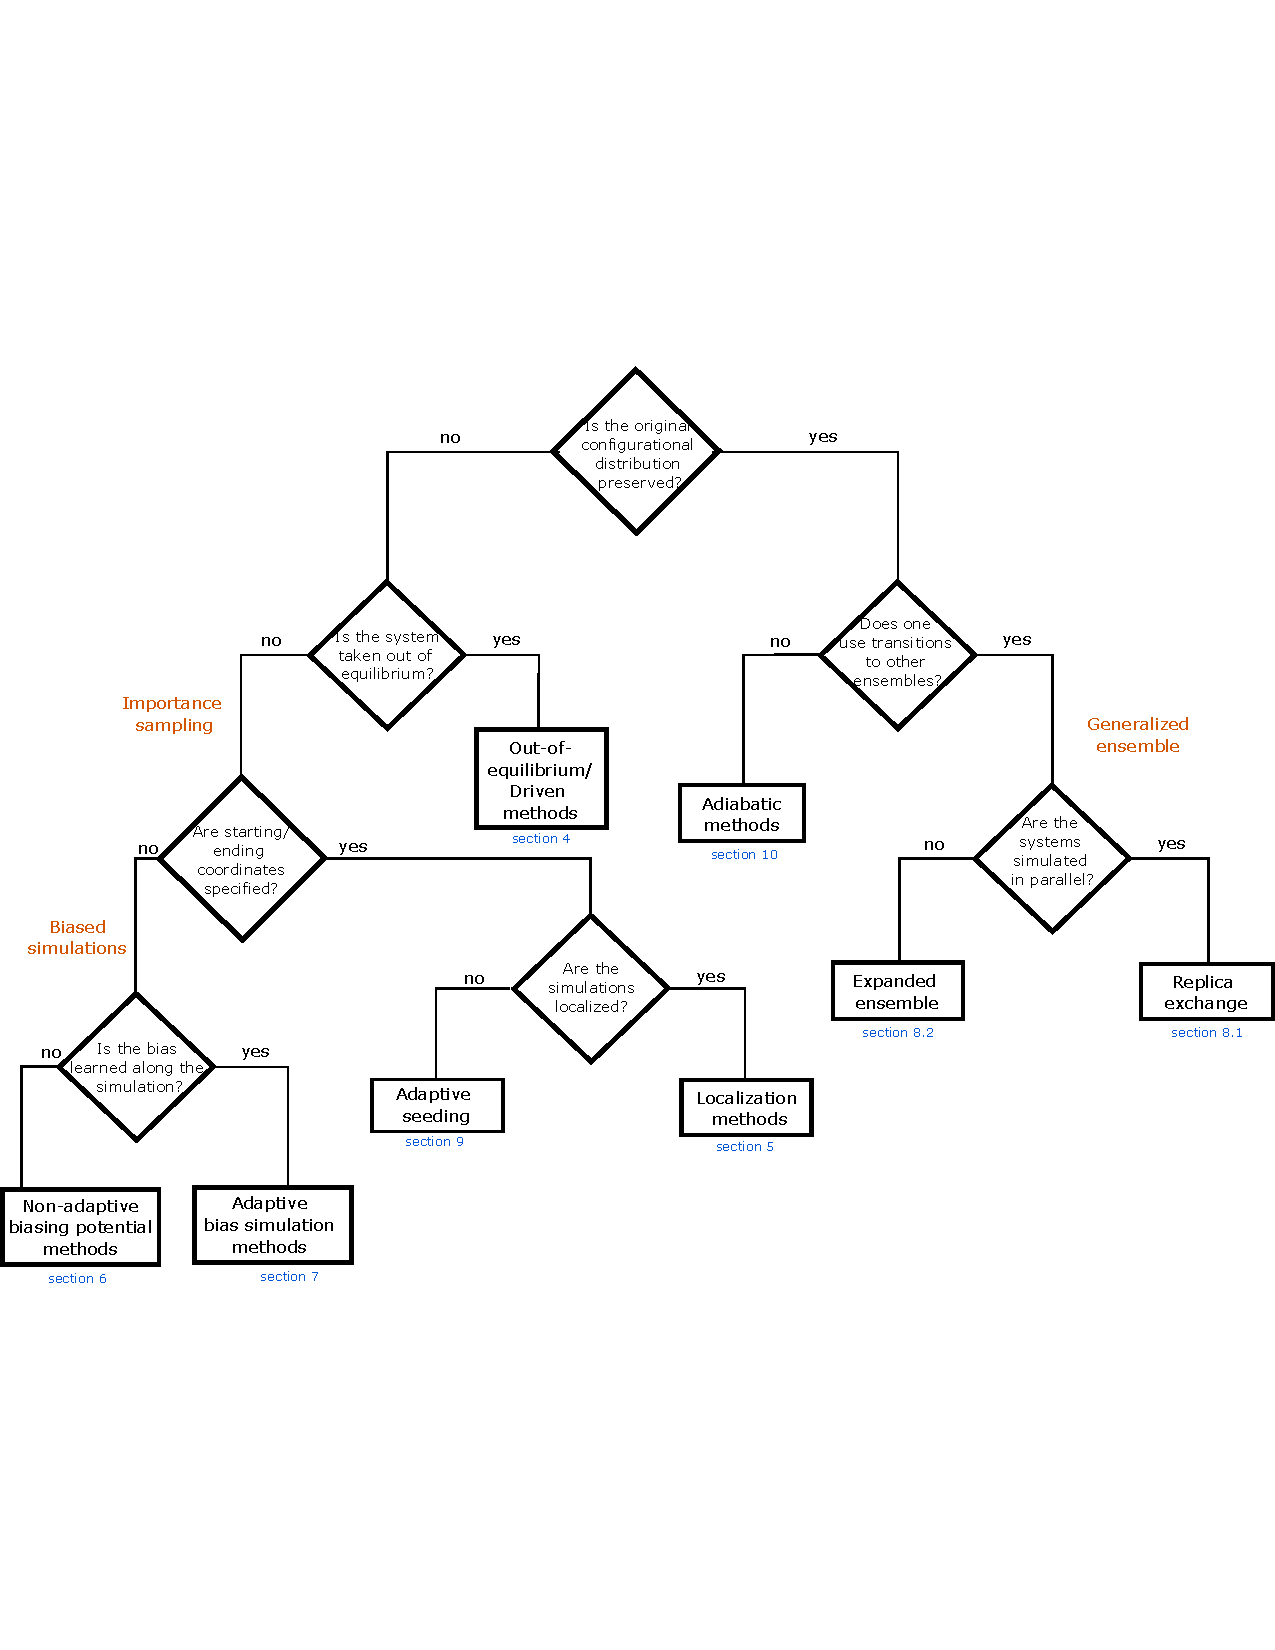
\includegraphics[scale=0.85]{Figures/Enhanced_sampling_sorting_final.pdf}
  \caption{An attempt at classifying enhanced sampling schemes, answering yes/no questions that delineate various strategies based on physical or statistical principles (black diamonds). The sorting algorithm results in eight different classes of methods (black boxes). The section of the review describing the family of methods is shown in blue below the corresponding box. Labels in orange refer to families of methods that can be grouped under an umbrella term.}
  \label{fig:scheme}
\end{figure*}

\begin{figure}[!htb]
  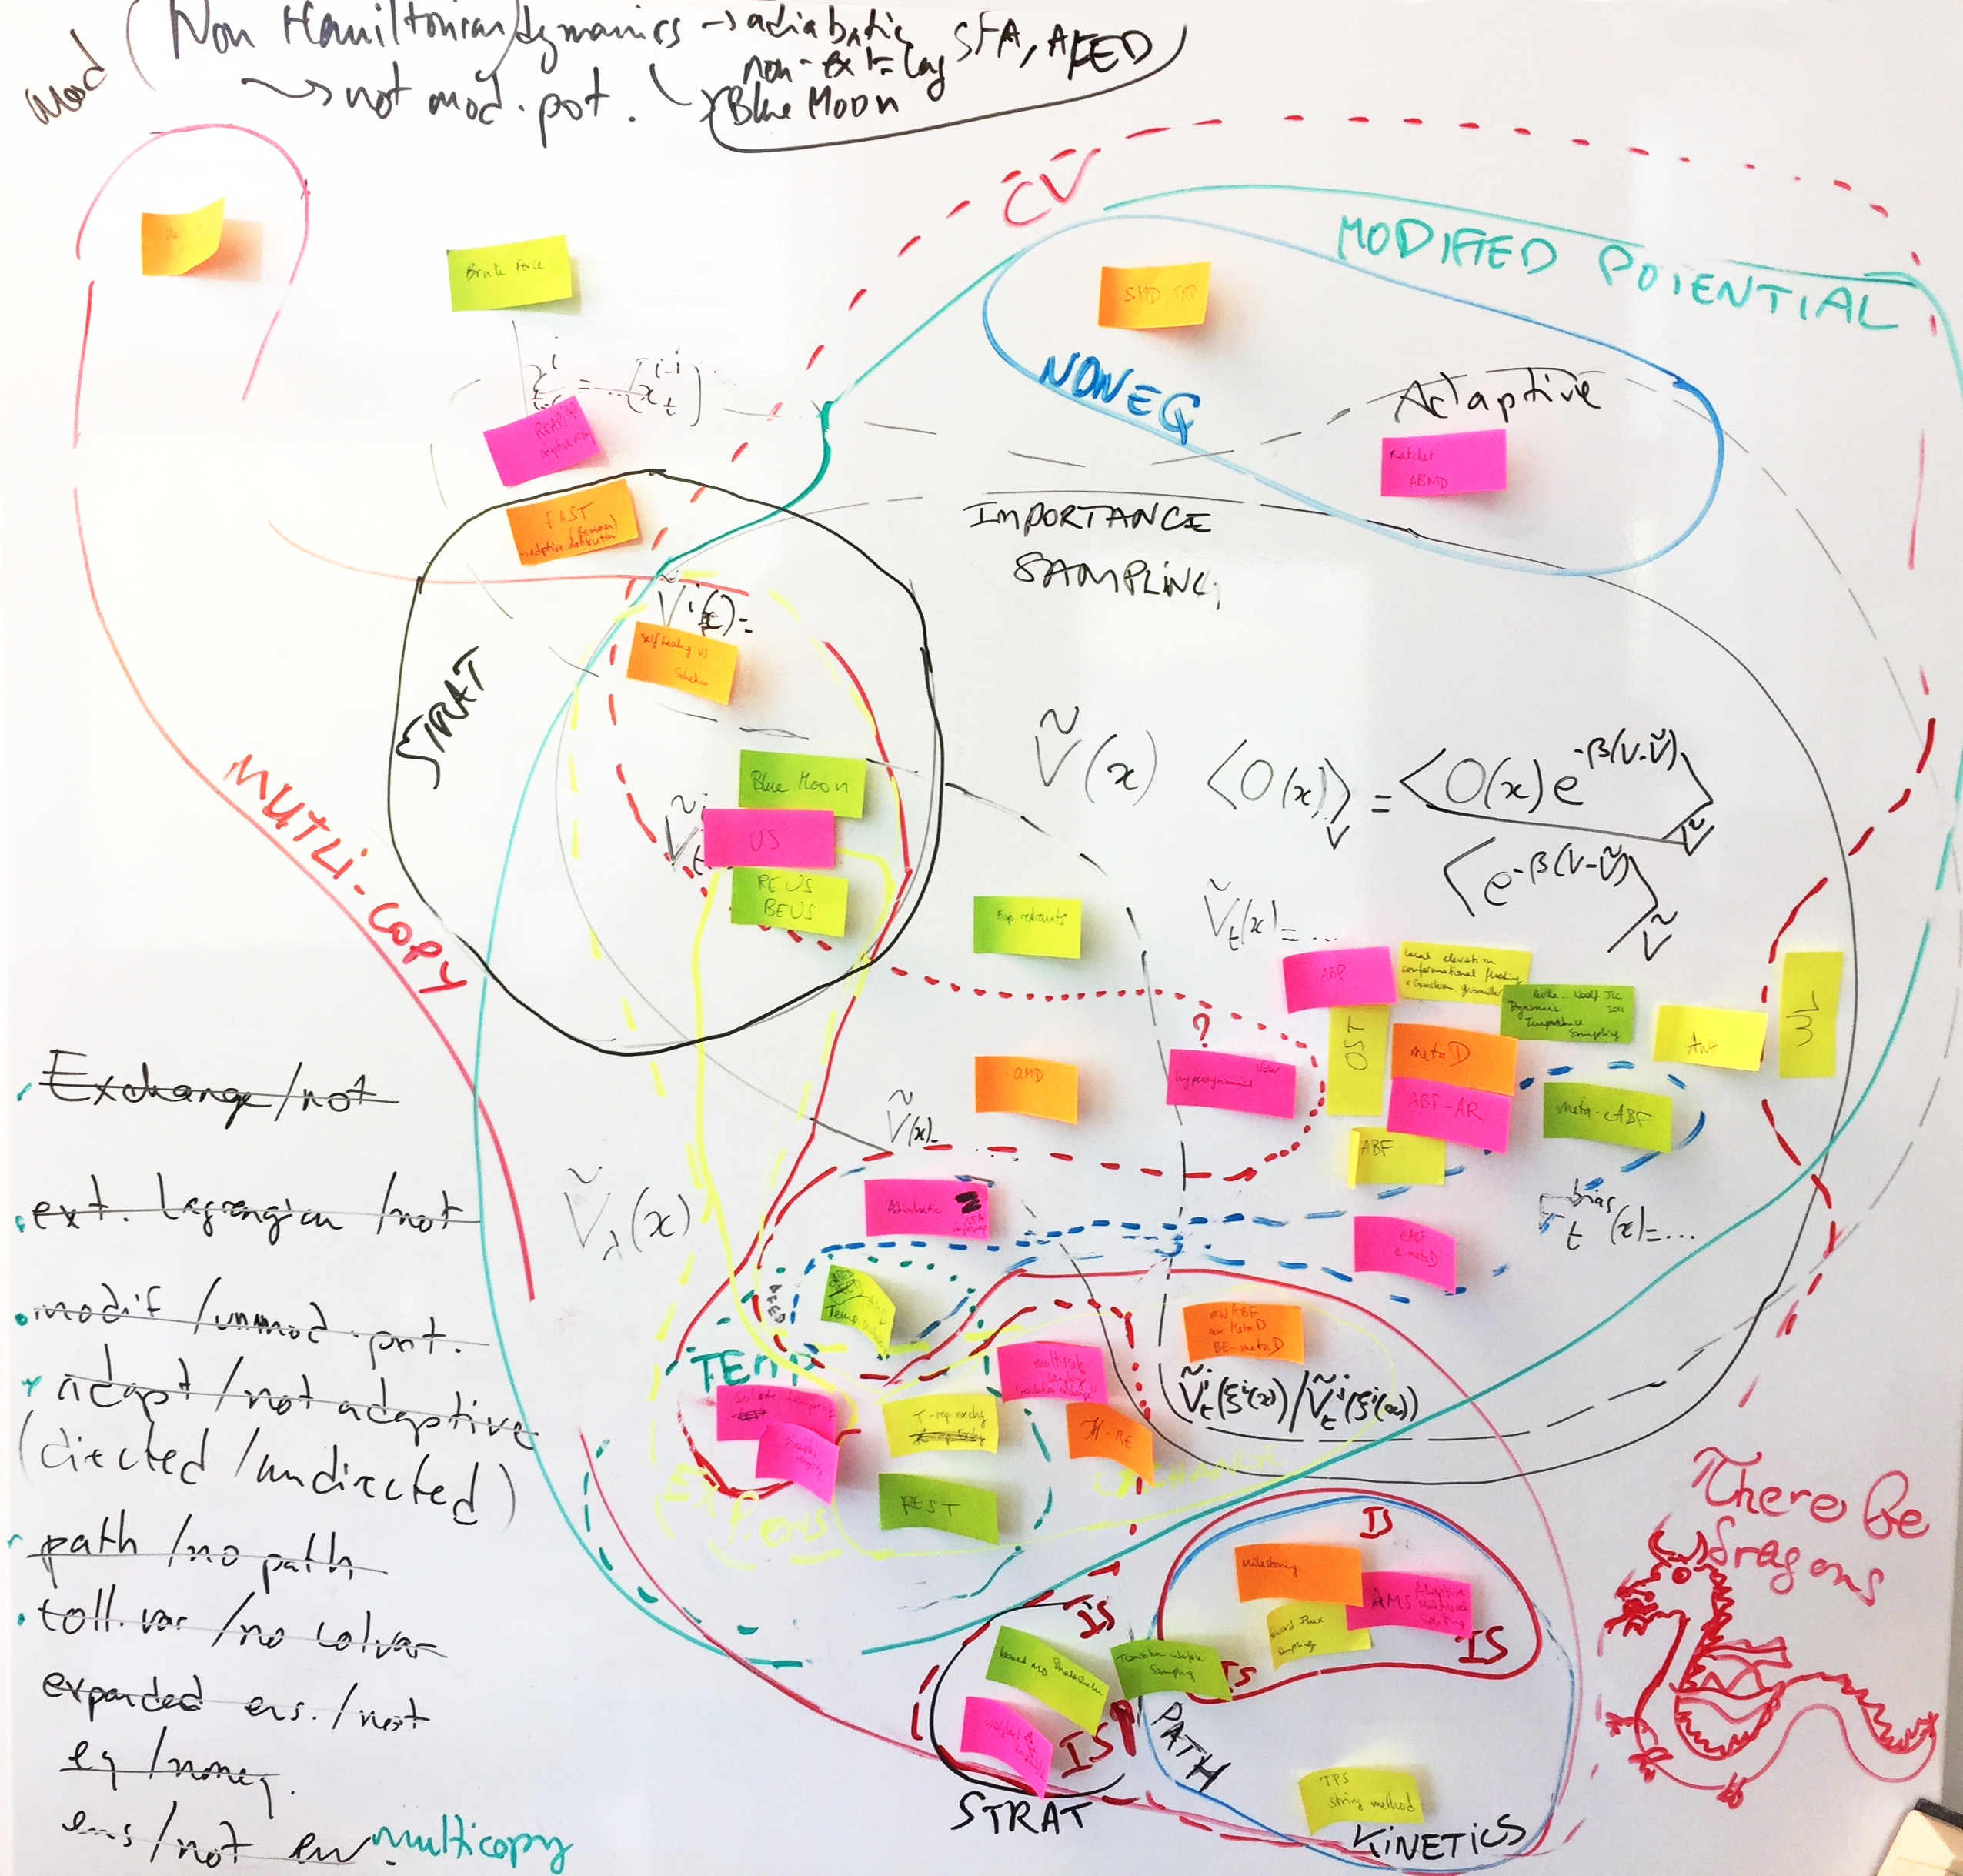
\includegraphics[width=0.99\columnwidth] {Figures/Venn_Diagram_Early_Attempt.jpeg}
  \caption{Early attempt at listing and classifying existing enhanced sampling schemes.}
  \label{fig:VennD}
\end{figure}

The next sections provide the background information needed to understand this scheme, starting with the notation used throughout the paper and a glossary in Section~\ref{sec:Notion_Notation}, a description of the free energy estimators that are used in various enhanced sampling schemes and will be referred to later in the text in Section~\ref{sec:fe_estimators}, and followed by the more detailed description of the various families of enhanced sampling methods that emerge from our classification. We then list a selection of hybrid schemes that combine different principles. Finally, we summarize the software packages (MD simulation codes and libraries) that are publicly and openly available to run these different types of enhanced sampling simulations.

\section{Useful notions and notations}
\label{sec:Notion_Notation}

One of the aims of this review is to use consistent notations to enable the reader to compare different methods, find similarities and differences across enhanced sampling
schemes. We introduce here the notation we will use throughout the paper. Note that given the existence of different notations in the literature, we have chosen the following one, while recognizing the validity of others. When especially crucial to understand the cited literature, we sometimes explicitly mention an alternative notation in following sections.

\subsection{Basic Notations}
\label{sec:Notation}
\begin{itemize}
\item Cartesian coordinates of atoms (or coarse-grain particles) denoted by $\vx$ and momenta denoted by $\vp$.
\item Potential energy function denoted by $U(\vx)$, defined by a classical molecular mechanics force field, various levels of electronic structure theory in an \emph{ab initio} dynamics framework, or a QM/MM hybrid and kinetic energy $K(\vp)$
\item Force on particles $\vF(\vx) = -\nabla_\vx U(\vx)$.
\item Absolute temperature $T$, inverse temperature $\beta = 1/(k_\mathrm{B} T)$.
\item \hypertarget{ref:AuxVar} {Extended (auxiliary) variable}: $\lambda$. This auxiliary variable can be a thermodynamic parameter, such as the temperature $T$ or the pressure $P$, or a parameter of the energy function $U_\lambda(\vx)$. The auxiliary variable can have a fixed value per simulation, can follow a pre-determined schedule, or can obey some dynamical equation of motion. It can have multiple dimensions, which we represent by the bold-faced vector $\boldsymbol{\lambda}$.

\end{itemize}

\subsection{Glossary of essential notions}
\label{sec:glossary}

\hypertarget{ref:Microstate} {\paragraph{Configuration or microstate}}
\index{configuration}
\index{microstate}
A single spatial arrangement of particles, represented by coordinates $\vx$. The set of possible configurations defines the configuration space $\Gamma$.
Configuration space augmented with the momenta variables is called the phase space, and therefore has twice the dimensionality. In many methods and calculations, we can take advantage of the fact that the momentum distribution obeys the analytical Maxwell-Boltzmann distribution at equilibrium.
In some cases, the  definition of configuration $\vx$ also includes the cell vectors of a periodic system (for example, in an isobaric ensemble).  This is used below where applicable.

We are using the original statistical mechanical definition of a microstate; we note that in the Markov State Modeling (MSM) literature, a microstate can also refer to an ensemble of configurations grouped together according to one or a set of order parameters, which is not intended here.

\paragraph{Molecular dynamics simulation}
\index{molecular dynamics}
A process that generates a trajectory, or sequence of configurations $\vx_t$.
The best-known classical dynamics is Hamiltonian dynamics:
\begin{equation}
\left\{
\begin{array}{ll}
    d\vx &= M^{-1} \vp \,  dt \\
    d\vp &= -\nabla_\vx U(\vx) \, dt
\end{array}
\right.
    \label{eq:md}
\end{equation}
where $M$ is the diagonal mass matrix.
Trajectories are often generated numerically using Verlet-style integrators.
A simplistic, discrete-time version of the above with time step $\delta t$ is:
\begin{equation}
\left\{
\begin{array}{ll}
    \delta \vx &= M^{-1} \vp \, \delta t \\
    \delta \vp &= -\nabla_\vx U(\vx) \, \delta t
    \label{eq:md_discrete}
\end{array}
\right.
\end{equation}

\hypertarget{ref:Ensemble} {\paragraph{Statistical ensembles from molecular dynamics}}
\index{ensemble}
Hamiltonian dynamics conserves mechanical energy, and can be used to sample from the microcanonical (constant number of particles $N$, constant volume $V$ and constant energy $E$, NVE) ensemble under an \hyperlink{ref:ergodic} {ergodicity} assumption.

Isothermal dynamics includes modifications that function as a thermostat, simulating the equilibrium with an external temperature bath at a target temperature T.
As a result, as long as the simulation is at or near equilibrium, its temperature fluctuates around T, and it samples the canonical ensemble (NVT).
An example of isothermal dynamics is \hypertarget{ref:Langevin} {Langevin dynamics}:

\begin{equation}
\left\{
\begin{array}{ll}
    d\vx &= M^{-1} \vp \,  dt \\
    d\vp &= \left(-\nabla_\vx U(\vx) - \gamma \vp \right) dt
    + \sqrt{ \frac{2 \gamma M}{\beta}} \; d\mathbf{W}_t
\end{array}
\right.
\end{equation}
where $\gamma$ is a friction coefficient and ${W}_t$ is a Brownian motion in dimension $3N$.

For the sake of intuition, consider a discrete-time version of Langevin dynamics:
\begin{equation}
\left\{
\begin{array}{ll}
    \delta\vx &= M^{-1} \vp \, \delta t \\
    \delta\vp &= \left(-\nabla_\vx U(\vx) - \gamma \vp + \sqrt{ \frac{2 \gamma M}{ \beta dt}} \, \mathbf{G} \right) \delta t
    \label{eq:Langevin_discrete}
\end{array}
\right.
\end{equation}
where $\mathbf{G}$ is a Gaussian-distributed stochastic 3N-vector of zero mean and variance 1.
Note that in practice, more sophisticated discrete Langevin integration schemes are used, which bring much better accuracy, stability, and performance~\cite{Skeel2002, Leimkuhler2012}.
Still, comparing the simple-minded Equations~\ref{eq:md_discrete} and \ref{eq:Langevin_discrete} shows that Langevin dynamics can be interpreted intuitively as similar to Hamiltonian dynamics, but including a modified force with added friction and stochastic collision terms. When $\gamma$ is zero, it reduces exactly to Hamiltonian dynamics.
Note that there are many other possible thermostats that can replace Hamiltonian dynamics, each with different numerical benefits and pitfalls. Note that some historic algorithms maintain an approximate target temperature, but do not sample from the canonical ensemble.
Isothermal-isobaric dynamics also includes a barostat, producing volume fluctuations consistent with a given target pressure $P$, and samples the isothermal-isobaric ensemble (NPT).
Again, there exists a variety of equations of motions with this property, and numerical algorithms implementing them. Langevin dynamics will be used as a basic example in later sections of this review.

\hypertarget{ref:Distribution}{\paragraph{Distribution}}

The Boltzmann distribution (which characterizes the canonical ensemble) in phase space has the following probability density:
\begin{equation}
\mu(\vx, \vp) = \frac{1}{Q} e^{-\beta (U(\vx) + K(\vp))}
\label{eq:BoltzmannDistr}
\end{equation}
where $ \displaystyle Q = \int e^{-\beta (U(\vx) + K(\vp))} d\vx d\vp$ is the normalization factor, known as partition function.

The physical meaning of $\mu$ is a probability per unit volume of $(\vx, \vp)$ space. The probability of a region of phase space $\Sigma$ is:
\begin{equation}
    P(\Sigma) = \int_\Sigma \mu(\vx, \vp) \, d\vx d\vp
\end{equation}

Most cases are described by a separable Hamiltonian, meaning that the energy is a sum of a potential term that depends only on positions and a kinetic term that depends only on momenta.
Then the momenta are statistically independent from the system configuration, hence their distribution is that of the ideal gas and does not bear significant information on any specific system.
This leads to a simple expression for the configurational distribution, where the momenta and kinetic energy do not appear:
\begin{equation}
\nu(\vx) = \int \mu(\vx, \vp) \, d\vp = \frac{1}{Z} \, e^{-\beta U(\vx)}
\end{equation}
where $Z$ is the configurational partition function. Sometimes, it may also be useful to define an unnormalized version of the configurational distribution, $q(\vx)$, such that $\nu(\vx) = \frac{1}{Z}q(\vx)$. There exist equivalent definitions of distributions for the isothermal-isobaric ensemble (NPT), which can be found in most statistical mechanics books.\cite{Zuckerman2010, Tuckerman2010}

Note that there are other notation conventions: in some texts and papers, $Q$ denotes the configurational partition function and $Z$ denotes the configurational and momenta partition function.


\paragraph{Macrostate}

Macrostates are experimentally distinguishable or measurable states of a system.
They can be described formally either in terms of the thermodynamic state variables ($E$, $T$, $P$, $V$, or parameters of the Hamiltonian) or by specifying specific regions of configuration space (that is, disjoint sets of microstates). A macrostate, besides being just a collection of microstates, also specifies a probability associated with each microstate that is contained in the microstate. The term ``thermodynamic state" is often used synonymously with macrostate, as the macrostates that we are most generally interested in studying with molecular simulation are macrostates that are completely defined by the specification of the macroscopic thermodynamic variables.

\paragraph{Free energy}
In the canonical \hyperlink{ref:Ensemble} {ensemble}, the Helmholtz free energy $F$ is a property of macrostate of a system, and is proportional to the logarithm of its partition function, which measures its statistical weight compared to other macrostates:
\begin{equation}
F \propto -\beta^{-1} \ln Z_{\Sigma} = -\beta^{-1} \ln \int_\Sigma e^{-\beta U(\vx)} \, d\vx,
\end{equation}
where the integration is done over a subset $\Sigma$ of configurational space corresponding to the macrostate. $F$ is thus a function of $\Sigma$, $U(x)$, and $\beta$, though often what the values of these variables is assumed by the context.

When using a classical energy function, $F$ is only defined up to an arbitrary additive constant.
In practice, this is not a limitation, as one is generally interested in free energy differences between two macrostates, rather than absolute free energies.
If two macrostates $\A$ and $\B$ can be distinguished experimentally, the ratio of their probabilities ($P_A = Z_A/Z$ and $P_B = Z_B/Z$) is an experimental observable, and so is the free energy difference:
\begin{align}
  \Delta F_{\A,\B} &= F_{\A} - F_{\B} \nonumber\\
    & = -\beta^{-1} \ln \frac{Z_{\A}}{Z_{\B}} \nonumber\\
  & = -\beta^{-1} \ln \frac{P_{\A}}{P_{\B}}
\end{align}

The Helmholtz free energy is sometimes notated $A$ in the literature. In this review, we will use $F$ for Helmholtz free energy, and the the symbol $A$ will be used for the \hyperlink{ref:FES} {free energy surface}. Gibbs free energy $G$ is the equivalent quantity in the isothermal-isobaric ensemble.

\hypertarget{ref:FEestimator} {\paragraph{Free energy estimator}}
An expression or algorithm that takes simulation data and estimates a numerical value for free energies or their differences. See Section~\ref{sec:fe_estimators} for a list and description of useful free energy estimators.

\hypertarget{ref:reduced} {\paragraph{Reduced quantities for homogeneous treatment of different ensembles}}

We define the reduced energy function $u_i(\vx)$
for state $i$ to be
\begin{eqnarray}
u_i(\vx) &=& \beta_i ( U_i(\vx) \;
+ p_i V(\vx)) \label{equation:reduced-energy}
\end{eqnarray}
where the pressure-volume term $p_i V(\vx)$ is only included in the case of a constant pressure ensemble.
Other terms may be added to generalize to other ensembles.
For each state $i$, $\beta_i$ is the inverse temperature, $U_i(\vx)$ the potential energy function (which may include biasing weights), $p_i$ the external pressure.
This formalism allows a very large number of different
situations to be described by the same mathematics.

The reduced free energy $f$ is defined as $f = \beta F$ for the canonical ensemble,
or $f = \beta G$ for the isothermal-isobaric ensemble.
Then all \hyperlink{ref:Distribution} {Boltzmann-like distributions} for the thermodynamic ensembles mentioned above are given in their unnormalized form as $q(\vx) = e^{-u(\vx)}$ and normalized form as
  $\nu(\vx) = e^{f-u(\vx)}$.


\hypertarget{ref:CV}{\paragraph{Collective variable}} A function $\xi$ mapping the full $n$ dimensions configurations $\vx$ to a lower-dimensional representation $\vz$ (sometimes denoted as $\mathbf{s}$ in the literature):
\begin{equation}
\vz = \xi(\vx)
\end{equation}
In the literature, the letter $\xi$ is sometimes used for both the function and the variable. The same goes for $\vz$ (and $\mathbf{s}$).

\hypertarget{ref:DimRed} {\paragraph{Dimensionality reduction}}
The process of finding a function $\xi$ mapping high-dimensional $\vx$ to low-dimensional $\vz$.

\hypertarget{ref:FES} {\paragraph{Free energy profile / surface / landscape}}
\label{sec:FES}
While free energy can be expressed as the logarithm of a partition function, a free energy surface (FES) is the logarithm of a \textit{partially integrated partition function}.
Given a chosen set of collective variables $\vz = \xi(\vx)$, this partially integrated partition function is, up to a normalization factor, the marginal probability density $\rho(\vz)$, and is obtained by integrating the Boltzmann density over all variables except $\vz$ (at constant $\vz$):
\begin{equation}
\label{eq:fes_definition}
    A(\vz) = -\beta^{-1} \ln \int
    \delta\left(\vz-\xi(\vx)\right) \, \nu(\vx)\, d\vx
    = -\beta^{-1} \ln \rho(\vz) .
\end{equation}

In practice, most free energy surface calculations concern a Helmholtz free energy, but Gibbs free energy surfaces could be computed as well. The difference is small, unless the transformation of interest entails a measurable change in overall density.

If two macrostates $\A$ and $\B$ correspond to domains of \hyperlink{ref:CV} {collective variable} space, then the probability ratio can be obtained from a free energy \hyperlink{ref:FES} {surface} $A(\vz)$ by integrating its exponential (the associated density) over the corresponding domains:
\begin{align}
  \Delta F_{\A,\B} &=
  -\beta^{-1} \ln \frac{Z_\A}{Z_\B}\\
  & =  -\beta^{-1} \ln
  \frac{\int_\A e^{-\beta A(\vz)} \, d\vz}
  {\int_\B e^{-\beta A(\vz)} \, d\vz}.
\end{align}

Similarly to other reduced quantities, one may define the reduced free energy surface
\begin{equation}
    a(\vz) = \beta A(\vz)
\end{equation}

Note that in \hyperlink{ref:ExpEns} {expanded ensemble} approaches, a free energy as a function of the extended variable $\lambda$ can be defined as:
\begin{align}
    A(\lambda) &= -\beta^{-1} \ln Z_\lambda
    \nonumber \\
    &= -\beta^{-1} \ln \int
    \nu(\vx, \lambda)\, d\vx
\end{align}

There is a very general relation between thermodynamic quantities (with the dimension of an energy) and probabilistic quantities.
The latter can be expressed as minus thermal energy ($-k_\mathrm{B} T = -\beta^{-1}$) times the natural logarithm of the former: this process is called Boltzmann inversion.
The main quantities discussed above are summarized in Table~\ref{tab:quantities}.


\begin{table}[]
\small
    \centering
\begin{tabular}{c|c}
probabilistic quantity & thermodynamic quantity  \\
$\bullet$ &   $-\beta^{-1} \ln(\bullet)$ \\
\hline
probability density $\nu(\vx)$  & potential energy  $U(\vx)$\\
$\downarrow$ &  \\
\textit{integrate over $\vx$ at constant $\vz$} & \\
$\downarrow$ &  \\
marginal probability density $\rho(\vz)$ & free energy surface $A(\vz)$ \\
$\downarrow$ &  \\
\textit{integrate over $\vz$ in $\Sigma$} & \\
$\downarrow$ &  \\
probability (measure) $P(\Sigma)$  & free energy  $F(\Sigma)$\\
\end{tabular}
    \caption{Relations between key statistical and thermodynamic quantities.
    The right column is $-\beta^{-1}$ times the logarithm of the left column.
    Probabilistic quantities are related by successive integration over larger slices of configuration space.}
    \label{tab:quantities}
\end{table}


The free energy surface can be interpreted as an effective energy for the collective variables.
The free energy surface is related to a probability density in the same way a free energy is related to the probability of a state (Table~\ref{tab:quantities}).
Beware, however, that a probability density is not a probability measure: a value of the density is not the probability of any particular event.
Whereas probability values are unitless and between 0 and 1, a probability density has units inverse $n$-dimensional volume (i.e., inverse of the unit of the coordinate variable in one dimension), and can take values greater than 1. The probability of a state is obtained from a probability density by integration over the relevant region of configuration space, and in a continuous configuration space, the probability of each individual configuration is zero.
A density is normalized: its integral over the whole space is unity.
Similarly, a free energy surface is not directly interpretable as a macroscopic free energy. Unlike a free energy, it is not an experimental observable.
Very importantly, free energy surfaces do not generally have a simple interpretation in terms of dynamics (e.g. free energy maxima may not be kinetic barriers), because of distortions due to the non-linear geometry of the variables.


\paragraph{Potential of Mean Force (PMF)}
Beware that this phrase is used in the literature in two different, incompatible meanings. The most common meaning nowadays is just the free energy surface as defined above.

Another one is the historic notion of PMF, which was first used to describe the structure of simple liquids.
The potential of mean force $W(r)$ between two particles was defined based on its radial distribution function $g(r)$, which is based on the probability density for the interparticle distance $r$, $\rho(r)$, divided by a normalization term ($r^2$) that makes it constant at large distances.
\begin{align}
    W(r) &= -\beta^{-1} \ln g(r) \nonumber \\
    &= -\beta^{-1} \ln \frac{\rho(r)}{r^2} + C  \nonumber \\
    &= A(r) + 2 \beta^{-1} \ln(r) + C,
    \label{eq:pmf_fes}
\end{align}
where $A(r)$ is the \hyperlink{ref:FES} {FES} along the interparticle distance and $C$ is an arbitrary constant.
The historic PMF and FES are therefore related, but distinct quantities.

The phrase ``potential of mean force'' describes very literally that $W(r)$ is a potential arising from an average force that would act on a particle at that location. In particular, it is zero in non-interacting systems (if $U(\vx) = 0$ for all $\vx$ then $W(r) = 0$ for all $r$), which is not generally the case for free energy surfaces.
For details, refer to Section~\ref{sec:fe_estimators:TI} on Thermodynamic Integration.

Here again, one may define the reduced version of $W(r)$:
\begin{equation}
    w(r) = \beta W(r)
\end{equation}

\paragraph{Multimodal distribution}
A probability distribution featuring many disconnected regions of high probability (each local maximum is a \textit{mode}) separated by regions of very low probability. Typically, if the dimension is high, most of the volume of configuration space has a very small probability.


\hypertarget{ref:ensemble_average} {\paragraph{Ensemble average}}

The ensemble average of an observable $O(\vx)$ which is a function of the configuration space is defined as:
\begin{align}
\langle O \rangle &= \int O(\vx, \vp) \mu(\vx, \vp) \, d\vx d\vp
\end{align}

Or if $O$ is only a function of configurations, then
\begin{align}
\langle O \rangle &= \int O(\vx) \nu(\vx) \, d\vx
\end{align}

All measurable thermodynamic quantities of interest are ensemble averages of some observable. For example, the total energy $U$ of a system is the expectation value of the Hamiltonian $\langle \bf{H} \rangle$. Furthermore, the marginal probability density $\rho(\vz)$ is an ensemble average of a Dirac $\delta$ ``function'', $\rho(\vz)=\langle \delta\left(\vz-\xi(\vx)\right) \rangle$ (see Equation~\ref{eq:fes_definition}).

\hypertarget{ref:ergodic} {\paragraph{Ergodic dynamics}}
The dynamics of a system is said to be ergodic if samples taken from any single, infinitely long trajectory describe the complete statistical properties of the dynamics.
This allows the estimation of ensemble averages by the time average or (\textit{ergodic average}).
If we want to compute the average of observable $O(\vx, \vp)$ according to distribution $\mu(\vx, \vp)$, and we can generate a discrete dynamics $(\vx_t, \vp_t)$ that is ergodic with respect to distribution $\mu$, then the ensemble average $\langle O \rangle$ can be estimated as a time average:
\begin{align}
\langle O \rangle &= \int O(\vx, \vp) \mu(\vx, \vp) \, d\vx d\vp
\nonumber \\
&\approx \frac{1}{N} \sum_{t=1}^N O(\vx_t, \vp_t) \text{ for sufficiently large $N$.}
\end{align}

More precisely:
\begin{equation}
   \langle O \rangle = \lim_{N \to \infty} \frac{1}{N} \sum_{t=1}^N O(\vx_t, \vp_t)
    \label{eq:ergodic}
\end{equation}

Solution-phase molecular dynamics of small molecules is nearly always ergodic in practice, and many biological and soft materials problems are as well: from here on, we consider only ergodic dynamics.
However, this is a theoretical notion that characterizes asymptotic behavior over infinitely long times (the limit in Equation~\ref{eq:ergodic}).
In practice, molecular dynamics simulations are often very short compared to the longest relaxations times, so that trajectories do not explore the full configuration space.
This situation is described as ``quasi-nonergodicity''.
Enhanced sampling methods target precisely this case, and aim to recover the statistical properties of ergodic dynamics from trajectories of limited duration.

\paragraph{Metastability and metastable states}
When a system resides in some some regions of configuration space for long times, with rare transitions between those regions, those regions are called metastable regions or metastable states. Metastable regions are typically modes of a multimodal distributions.

\hypertarget{ref:biasingE} {\paragraph{Biasing and biased energy}}
A biasing energy is an extra energetic term $U^\mathrm{bias}$ added to obtain a potential energy $\tilde{U}(\vx)$ biased to behave a certain way:
\begin{equation}
\tilde{U}(\vx) =  U(\vx) + U^\mathrm{bias}(\vx).
\end{equation}
In molecular dynamics, a bias energy
$U^\mathrm{bias}(\vx)$ gives rise to a bias force $\vF^\mathrm{bias}(\vx) = -\nabla_{\vx} U^\mathrm{bias}(\vx)$, so that the total biased force $\tilde{\vF}(\vx)$ is
\begin{equation}
\tilde{\vF}(\vx) = -\nabla_{\vx} \tilde U(\vx) = \vF(\vx) + \vF^\mathrm{bias}(\vx)
\end{equation}
The bias $U^\mathrm{bias}(\vx)$ is often a function of low-dimension \hyperlink{ref:CV} {collective variable}s $\vz = \xi(\vx)$, and can be written $U^\mathrm{bias}(\vx) = U^\mathrm{bias}(\xi(\vx)) = U^\mathrm{bias}\circ \xi(\vx)$ so that in this case, the biased potential energy function is $\tilde U= U + U^\mathrm{bias}\circ \xi$.
The resulting biasing force on atoms is calculated using the chain rule:
\begin{align}
\tilde{\vF}(\vx) &= -\nabla_{\vx} \tilde U(\vx) \\
&= \vF(\vx) -\nabla_{\vx} [ U^\mathrm{bias}(\xi(\vx))]\\
\tilde{\vF}(\vx)&= \vF(\vx) - \left . \frac{dU^\mathrm{bias}}{dz}\right |_{z=\xi(\vx)} \; \nabla_{\vx}\xi(\vx)
\end{align}
This requires the computation of the gradient $\nabla_{\vx}\xi(\vx)$ of the collective variable with respect to atomic Cartesian coordinates.

\hypertarget{ref:IS} {\paragraph{Importance Sampling}}
\label{sec:importance_sampling} A family of methods where a different probability distribution $\tilde\nu(\vx)$ from the target one is sampled, in such a way that the ratio of the two distributions is known or estimated numerically, typically up to a multiplicative constant.
The biased probability density arises from a biased potential energy function or another modification of the Hamiltonian of the system:
\begin{equation}
\tilde \nu(\vx) \propto \exp(-\beta \tilde U(\vx))
\end{equation}

The name refers to the idea of favoring sampling of the regions of importance, or if they are unknown, to flatten sampling towards a more uniform distribution.
Importance sampling methods include the biasing potential and biasing force methods (\hyperlink{ref:Adaptive} {adaptive} or not), localization methods and adaptive \hyperlink{ref:Seeding} {seeding} methods described in Sections~\ref{sec:localization}, \ref{sec:biasing_potential}, \ref{sec:AdaptiveBiasSimulations} and \ref{sec:seeding}.

As explained below, unbiased properties of the original distribution may be obtained by \hyperlink{ref:Reweighting} {reweighting} from the modified, sampled distribution to the desired distribution.
In practice, the  sampled distribution is chosen to emphasize samples that contribute strongly to the averages of interest, making the reweighted average over samples from the modified distribution a low-variance estimator.


\hypertarget{ref:Reweighting} {\paragraph{Reweighting}}
Calculating averages and free energies of one distribution using samples from another one. This distribution may be one explicitly generated by a biased simulation, or one that is a mixture of several sampled distributions~\cite{reweighting_mixture_distribution}.
Here the observed distribution is $\tilde \nu$ and the original, unbiased distribution $\nu(\vx)$ is obtained using:
\begin{equation}
\nu(\vx) \propto \tilde\nu(\vx) e^{\beta U^\mathrm{bias}(\vx)},
\end{equation}
where $U^\mathrm{bias}(\vx)$ is the bias potential.

More practically, the average of an observable $O(\vx)$ over the canonical distribution is estimated by:
\begin{equation}
\langle O(\vx) \rangle = \frac{\langle O(\vx) e^{\beta U^\mathrm{bias}(\vx)} \rangle_{\tilde U}}
{\langle e^{\beta U^\mathrm{bias}(\vx)} \rangle_{\tilde U}},
\end{equation}
where the ensemble averages on the right side are taken according to the canonical distribution arising from the biased potential energy $\tilde U(\vx)$.


\paragraph{Biased CV distribution}
Under the influence of a bias potential acting in \hyperlink{ref:CV} {CV} space $U^\mathrm{bias}(\vz)=U^\mathrm{bias}(\xi(\vx))$, the \hyperlink{ref:CV} {CV} will follow a biased \hyperlink{ref:CV} {CV} distribution given by
\begin{equation}
\tilde \rho(\vz) \propto e^{-\beta \left[
A(\vz) + U^\mathrm{bias}(\vz)
\right]}
\end{equation}

\hypertarget{ref:targetdist}{\paragraph{Target distribution}}
Common in some enhanced sampling methods is the concept of a target distribution. This represents a desired probability distribution over a (set of) variable that an enhanced sampling simulation is trying to achieve. The target distribution can be in the space of some collective variables (normally, the ones being biased) or another space such as the state space in $T$ or along an auxiliary variable $\lambda$. In some methods, the target distribution is set by the user. In others, the target distribution can be inferred from experimental observations. A common choice is to set the target distribution to be uniform over the variables or states of interest, with all values sampled equally. However, most methods theoretically support the usage of any given non-uniform target distributions if the user desires.

\hypertarget{ref:Balance} {\paragraph{Detailed Balance and Balance}}
Detailed balance is a constraint on the way moves from a given state of a system to another one are performed.  If $i$ and $j$ are two states, then detailed balance requires that
\begin{equation}
\frac{P(i)}{P(j)} = \frac{P_{i\rightarrow_j}}{P_{j\rightarrow_i}},
\end{equation}
where $P(i)$ and $P(j)$ are the desired probabilities of $i$ and $j$, and $P_{i\rightarrow j}$ and $P_{j\rightarrow i}$ are the probabilities of transitioning from state $i$ to $j$ and state $j$ to $i$ during some process.
Generally, physical systems obey detailed balance, and most common simulation methods, such as molecular dynamics or Metropolis Monte Carlo obey detailed balance, and thus preserve the overall probability distribution of the system.

Balance is a weaker requirement~\cite{deem:jcp:1999:balance}, and is merely that the desired probability distribution is preserved. This can be done without forcing the ratio of the fluxes between states being equal to the ratio of the probabilities of two states, as is the case in detailed balance.  For example, you could have a cycle of flux between three states $i$,$j$, and $k$, and still preserve the probability distribution.  Proving a given set of ways to perform moves between states obeys balance is usually significantly harder than proving that a set of moves preserves detailed balance.
However, studies have shown that it is often possible to obtain better sampling through states with algorithms that only obey balance rather than detailed balance~\citep{deem:jcp:1999:balance,Faizi:JCTC:2020}.

\hypertarget{ref:MetropolisMonteCarlo} {\paragraph{Metropolis Monte Carlo}}
A Metropolis Monte Carlo step makes some change in the system in a way that preserves the underlying probability distribution (usually the Boltzmann distribution).  The simplest rule is to propose some new coordinate $\vx^\prime$, and change from $\vx$ to $\vx^\prime$ with probability:
\begin{eqnarray}
P(\vx\rightarrow \vx^\prime) = \min\left\{1, e^{-(u(\vx^\prime)-u(\vx))}\right\}
\label{eq:bal}
\end{eqnarray}
This means that the move always occurs if the energy is lowered (probability is increased), and sometimes occurs if the energy is higher, with the probability given in Equation~\ref{eq:bal}.
In order for this to preserve the underlying Boltzmann distribution, proposals must be made in a symmetric way, such that the the probability of proposing $\vx$ when at $\vx^\prime$ is the same as the probability of proposing $\vx^\prime$ when at $\vx$. This is satisfied by simple rules like translating or rotating particles a symmetric amount from the current position, but care must be taken for more complex coordinate transformations like torsional displacement volume changes, or polymer chain moves~\cite{Siepmann_mp_1992}.  It is in fact possible to choose new states with asymmetric or biased probabilities if those biases and asymmetries are properly accounted for; this generalization is called a \emph{Metropolis-Hastings} step~\cite{Hastings_biometrika_1970}.

In addition, the Metropolis (or Metropolis-Hastings algorithms), can also be used to propose new parameters, such as a change in the temperature of the system, or a change in the potential energy of the system. Because the free energy of the system will change when a parameter of the system is changed, then other correction factors must be included.

\hypertarget{ref:GibbsSampler} {\paragraph{Gibbs Sampler}}
\hyperlink{ref:MetropolisMonteCarlo} {Metropolis Monte Carlo} steps are ways to move from one state of the system to another, considering one trial step at a time.  The Gibbs sampler~\cite{shirts_gibbssamp} is a  way to move to another state considering many trial states simultaneously. It is generally used when there are two (or more) different types of variables defined in the system that could be changed, $x$ and $y$, so the probability of the system is defined by $\nu(x,y)$. The Gibbs sampler is defined by taking steps in $x$ first and then $y$, by the following algorithm:
\begin{enumerate}
\item Start at $x_i$,$y_i$.
\item Pick a variable to change randomly with some frequency $f$, such that $f(x)+f(y)=1$.
\item If you choose $x$, pick a new $x$ from the conditional distribution $\nu(x|y_i)$, i.e. the probability of $x$ given $y_i$.
\item If you choose $y$, pick a new $y$ from the conditional distribution $\nu(y|x_i)$, i.e. the probability of $x$ given $y_i$.
\item Repeat.
\end{enumerate}
Any method to pick $x$ and $y$ from the distribution can be used, including \hyperlink{ref:MetropolisMonteCarlo} {Metropolis Monte Carlo}. The algorithm could be generalized to more than two variables, by randomly choosing each of the variables. Interestingly, one can alternate between variables deterministically (first pick $x$, then pick $y$, then pick $x$ again, or pick $x$ 100 times, then $y$, then $x$ 100 times again) and the results will not satisfy detailed balance, but they will still satisfy balance, which means the distribution $\nu(x,y)$ will be preserved.
To be concrete, let us assume one variable is the coordinate $\vx$, and the other is the temperature $T$. Then one implementation of the Gibbs sampler, one would carry out simulations in $\vx$ using molecular dynamics in the NVT or NPT ensemble for a certain number of steps, then perform a move in $T$ space using an algorithm that generates a new $T$ from $\nu(T|\vx)$, while keeping the coordinates constant.

\hypertarget{ref:GenEns} {\paragraph{Generalized ensemble}}
Generalized ensemble methods encompass \hyperlink{ref:ExpEns} {expanded ensemble methods} and \hyperlink{ref:ReplEx} {replica exchange} methods.

\hypertarget{ref:ExpEns} {\paragraph{Expanded ensemble}}
While a usual statistical-mechanical ensemble describes one set of macroscopic conditions, an expanded (or extended) ensemble allows for additional degrees of freedom (physical or non-physical) to vary. Physical parameters encompass, for example, the temperature. Non-physical parameters are characterized as ``alchemical'', and describe the transition between Hamiltonians representing different molecular systems: typically the change is either changing a molecule into another one, or decoupling a molecule from its environment.
Alchemical transformations are often used to estimate free energies of binding or solvation.
An expanded ensemble may be sampled mainly in two ways.
The first option is to run a collection of simulations (replicas, $i$) among which an \hyperlink{ref:AuxVar} {auxiliary parameter} $\lambda_i$ takes a discrete set of values.
In replica $i$, the dynamics of coordinates $\vx_i(t)$ are then propagated under a potential energy $U_{\lambda_i}(\vx_i)$ or at inverse temperature $\beta_i$.
The second option is to propagate $\lambda_i$ as an additional dynamic variable (see \hyperlink{ref:ExtL} {Extended Lagrangian}).

\hypertarget{ref:ExtL} {\paragraph{Extended Lagrangian dynamics, $\boldsymbol\lambda$ dynamics}}
A special case of \hyperlink{ref:ExpEns} {expanded ensemble} simulation, whose equations of motion include \hyperlink{ref:AuxVar} {``fictitious'' (auxiliary) dynamical degrees of freedom} $\lambda$ that are not the spatial coordinates of physical objects or the associated momenta.
To sample the canonical distribution of $(\vx, \lambda)$, they can be propagated following e.g. \hyperlink{ref:Langevin} {Langevin dynamics}:

\begin{equation}
\left\{
\begin{array}{ll}
d\vx &= M^{-1} \vp \, dt\\
d\vp &= \left(-\nabla_\vx U^\text{ext}(\vx,  \lambda) - \gamma \vp \right) dt
    + \sqrt{ \frac{2 \gamma M}{\beta}} \; d\mathbf{W}_t\\
d\lambda &= m_\lambda^{-1} p_\lambda \, dt \\
dp_\lambda &= \left(-\frac{\partial U^\text{ext}(\vx, \lambda)}{\partial \lambda} - \gamma_\lambda p_\lambda \right) dt
    + \sqrt{ \frac{2 \gamma_\lambda m_\lambda}{ \beta }} dW_t
\end{array}
\right.
\end{equation}

where $m_\lambda$ is a fictitious mass associated to $\lambda$.
While the two phrases are essentially synonymous, the term $\lambda$-dynamics is mostly used when a continuous dynamic variable $\lambda$ connects physically meaningful, and sometimes discrete, states, such as in alchemical transformations.
On the other hand, the term extended Lagrangian is more often used when  the fictitious coordinate $\lambda$ follows a \hyperlink{ref:CV} {collective variable} $\xi(\vx)$, typically coupled through a harmonic potential: $U^\text{ext}(\vx, \lambda) = U(\vx) + \frac{k^\mathrm{ext}}{2}|\xi(\vx)-\lambda|^2$.


\paragraph{Temperature-based sampling} Refers to enhanced-sampling methods relying on an increased temperature $\tilde T$ to reduce metastability. This can be done on some replicas within a set of replicas, on some fraction of the time within a given trajectory, or effectively on some fraction of the system by selective scaling of potential energy terms.
In the latter case, if $U = U^\mathrm{unscaled} + U^\mathrm{scaled}$, scaling $U^\mathrm{scaled}$ to reach effective inverse temperature $\tilde \beta = 1/(k_\mathrm{B} \tilde T)$ gives an expression of the bias potential $\tilde U$:
\begin{equation}
\tilde U = U^\mathrm{unscaled} + \frac{\tilde \beta}{\beta} U^\mathrm{scaled}.
\end{equation}


\hypertarget{ref:ReplEx} {\paragraph{Replica exchange}} \hyperlink{ref:GenEns} {Generalized ensemble} methods that allow for exchanging configurations between replicas, usually according to criteria that guarantee that each replica samples from a well-defined distribution. Described in more detail in Section~\ref{sec:generalized-ensemble}.

\hypertarget{ref:AdiabaticDyn} {\paragraph{Adiabatic dynamics}}
A dynamics where selected degrees of freedom are assumed to not exchange energy with the rest of the system.
This can be achieved if these degrees of freedom are decoupled from the rest of the system, and evolve effectively independently.

\hypertarget{ref:Driven} {\paragraph{Driven simulations}} Refers to simulations with a time-dependent bias potential $U^{\mathrm{bias}}_t(\vx)$ or force $\vF^\mathrm{bias}_t(\vx)$ following a pre-determined schedule.

\paragraph{Out-of-equilibrium system} A system that has not reached its steady state, either because it is considered on a time-scale smaller than its relaxation time-scales, or because it is \hyperlink{ref:Driven} {driven} by time dependent forces which maintain it out of equilibrium.

\hypertarget{ref:OutOfEq} {\paragraph{Out-of-equilibrium method}}
A simulation protocol that does not generate trajectories that sample from the canonical ensemble associated with a given potential energy function.
Instead, initial and boundary conditions are given, as well as a possibly time- and history-dependent potential energy function or force schedule. The statistics of the generated trajectories and configurations are determined by these conditions.
Unlike the canonical distribution, however, there is no general closed-form expression for the resulting out-of-equilibrium distributions of trajectories or configurations.

\hypertarget{ref:Seeding} {\paragraph{Seeding}}
A strategy where the configuration space covered by a set of (relatively short) simulations is governed by the choice of their starting conditions.
This strategy is typically used to increase the diversity of the samples produced, despite the internal correlation of each trajectory (see Section~\ref{sec:seeding}).


\hypertarget{ref:Adaptive} {\paragraph{Adaptive method}}
A simulation algorithm whose parameters are adjusted (``adapted'') along the simulation time based on the history of the simulation $(\vx_s, \vp_s), s\in [0, t]$.
This can take the form of a time-dependent bias potential $U^\mathrm{bias}_t(\vx)$ or force $\vF^\mathrm{bias}_t(\vx)$, or branching decisions to stop or launch simulation instances.
See Sections~\ref{sec:AdaptiveBiasSimulations} or \ref{sec:seeding}.

\hypertarget{ref:FEP} {\paragraph{Free energy perturbation - FEP}}
\label{FEP}

In free energy perturbation, one considers a simulation at equilibrium with respect to potential energy $U_\A$. Instantaneously switching to a different potential energy $U_\B$ (without any relaxation), one obtains a ``comparison energy'', the difference in energy between the two states for each configuration~$\vx$, $\Delta U_{\A\B}(\vx) = U_\B(\vx) - U_\A(\vx)$.

The free energy difference $\Delta F_{\A\B}$ can be obtained as an exponential average (see Section~\ref{sec:fe_estimators:EXP}) \cite{Zwanzig1954}
\begin{equation}
e^{-\beta \Delta F_{\A,\B}} = \left\langle e^{-\beta \Delta U_{\A,\B}}\right\rangle_\A
\end{equation}
where $\langle \;...\; \rangle_\A$ indicates an ensemble average in state $\A$.
By extension, the phrase FEP is sometimes used to refer to the free energy estimator itself.

\section{Free energy estimators}
\label{sec:fe_estimators}

Recovering the original statistical ensemble often requires estimating a free energy. For some methods, the \hyperlink{ref:FEestimator} {free energy estimator} is central to the enhanced sampling scheme, while for others, it is a post-processing tool. This section provides a concise presentation, but extensive reviews can be found elsewhere~\cite{cchipot07:molsim,doi:10.1142/p579,Paliwal_comparison_2011,shirts_comparison_2005,Klimovich_Shirts_Mobley_2015}.

\hyperlink{ref:FEestimator} {Free energy estimators} are expressions that are used numerically to compute free energy differences or free energy \hyperlink{ref:FES} {surfaces} from quantities that are available in simulations (configurations, energies, and forces).
The important properties of an estimator are its accuracy (\textit{bias}: how far off the real value it is given infinite, ideal sampling) and precision (\textit{variance}: how much it fluctuates given a finite amount of noisy data).

In this section we consider estimators for:
\begin{itemize}
    \item free energy as a function of a Hamiltonian parameter (auxiliary variable) $\lambda$, which the energy $u_\lambda$ depends on, or
    \item free energy \hyperlink{ref:FES} {surface}s as a function of a \hyperlink{ref:CV} {collective variable} (or a vector of variables) $\vz = \xi(\vx)$.
\end{itemize}

For generality, \hyperlink{ref:reduced} {reduced} units are used.

\subsection{Directly measured ratios, histograms}

Given a set of sampled configurations that visits two states $i$ and $j$, their free energy difference $f_{ij}$ can be estimated by direct Boltzmann inversion, approximating Equation~\eqref{eq:BoltzmannDistr}:
\begin{equation}
\Delta f_{ij} = -\ln \frac{N_j}{N_i}
\label{eq:boltzmann_inversion}
\end{equation}
where $N_i$ and $N_j$ are the numbers of observed configurations in states $i$ and $j$.
This is only true if the simulation samples the equilibrium between states $i$ and $j$, or equivalently, if it is long enough such that many transitions between those states have been observed~\cite{No2009}. If a list of several states is defined, then estimates from neighboring states can be chained to compute relative free energies for the entire list of states.
If the states are defined as bins along \hyperlink{ref:CV} {collective variable}s, this yields a (discretized) free energy \hyperlink{ref:FES} {profile} along those variables.
This idea extends to the calculation of continuous probability distributions and free energy surfaces. In that case, the probability distribution can be estimated using a kernel density estimator (KDE)~\cite{Westerlund2017}.

% Coverage of the states of interest can be improved by stratification (section~\ref{sec:localization}), in which case several simulated trajectories have to be pieced together to form an unbiased set of samples. Given sufficient overlap, the proper weights to be applied to each trajectory can be estimated using the methods described below.

Convergence of this ratio can be accelerated by \hyperlink{ref:IS} {importance sampling}: adding \hyperlink{ref:biasingE} {biasing} potentials $u^{bias}_i$ and $u^{bias}_j$, with $\Delta u^{bias}_{ij}=u^{bias}_j - u^{bias}_i$.
If the biases have constant values over each state, the free energy can be estimated by including a simple bias correction, e.g. \hyperlink{ref:Reweighting} {reweighting}:
\begin{equation}
\Delta f_{ij} = -\ln \frac{N_j}{N_i} - \Delta u^{bias}_{ij}
\label{eq:boltzmann_inversion_biased}
\end{equation}

\subsection{Estimating free energies from the transition count matrix\label{sec:transtion_matrix}}

The transition probabilities along one or more discretized \hyperlink{ref:CV} {CVs} can be used to build a transition probability matrix containing either the transitions from a state $i$ to a state $j$, or the probabilities $P_{ij}$ of performing the transition.

The free energy \hyperlink{ref:FES} {landscape} $A(\vz)$ can be derived as the negative logarithm of the stationary distribution $\nu(\vz)$, obtained by iterating over the discretized master equation
\begin{equation}
   \nu_i(t + \delta t) = \nu_i(t) + \sum_{j \neq i} \nu_j(t) P_{ji} - \nu_i(t) P_{ij}.
\end{equation}

Indeed, convergence of probability distributions is slow because the samples extracted from molecular dynamics simulations are correlated. By taking into account the conditional probability distribution (probability of an event happening given previous history), the statistical dependency of the MD trajectory is taken into account~\cite{No2007,Zhu2011,Rosta2014}. Note that free energy estimated directly from population ratios will be biased if too few transitions have been observed between states~\cite{No2009}.

If one is considering a simulation that allows transitions between two thermodynamic states $i$ and $j$, such as in an expanded ensemble simulation, then this implies the average of the transition probabilities between states is equal to the ratio of the partition functions between the states of interest \cite{deOliveira:EPJB:1998,Wang:JoSP:2002,escobedo_transition_2006}. Specifically:
\begin{equation}
e^{f_j-f_i} = \frac{Q_i}{Q_j} = \frac{\left \langle  P_{i\rightarrow j}(x)\right\rangle}{\left \langle P_{j\rightarrow i}(x) \right \rangle}
\end{equation}
where $P_{i\rightarrow j}(x)$ is the probability of accepting a move from state $i$ to state $j$ proposed from configuration $\vx$. For simplicity we assume that the probability of moves proposed from $i$ to $j$ is equal to the probability of transition from $j$ to $i$; more general transitions can also be included~\cite{escobedo_transition_2006}. We can construct a matrix of all possible transitions between any pair of states; hence we can call this a transition count matrix or \textit{transition matrix}.

Typically, this averaging is carried out over the transitions that were actually observed. However, this average can be performed over transitions \emph{that were not actually performed}. If one calculates the probability that the transition would occur even when a move is not made, it can be included in the average as well.

One can even compute this average of transition probability distributions using a different type of  probability distributions than one actually uses to carry out steps between ensembles. For example, one can show that the Metropolis criterion $(\mathrm{min} \{1,e^{-u_j+u_i})\})$ is more efficient to use as a move between two states but the Barker criteria $\left(\frac{e^{-u_j}}{e^{u_j}+e^{u_i}}\right)$ is more efficient to calculate free energies~\citep{Liu:Biometrika:1996}.

An even more accurate estimation of the free energies can be achieved by building a Markov State Model (MSM) from the transition count matrix, whereby the probability of each state is computed as the leading eigenvector of the transition matrix. In this case, it may not be necessary for single simulations to sample the entire state space, as long as each of the transitions individually is estimated accurately.

\subsection{Thermodynamic Integration (TI)}
\label{sec:fe_estimators:TI}

Thermodynamic Integration is the principle that the derivative of a free energy with respect to a continuous parameter can be expressed as an ensemble average of the derivative of the energy with respect to the same parameter.

\paragraph{TI along an alchemical parameter} In some cases, the potential energy is a function $u_\lambda$ of a smooth coupling parameter $\lambda$ that connects all states of interest (e.g. in alchemical perturbations).
This defines a continuous free energy $f_\lambda$, the derivative of which is the ``mean force'' at a fixed value of $\lambda$:
\begin{equation}
\frac{\mathrm{d}f}{\mathrm{d}\lambda} =\left\langle \frac{\partial u_\lambda}{\partial \lambda} \right\rangle_\lambda
\label{eq:TI1}
\end{equation}

If states $i$ and $j$ correspond to values $\lambda_i$ and $\lambda_j$ of the continuous coupling parameter, then $\Delta f_{ij}$ is
\begin{equation}
\Delta f_{ij} = \int_{\lambda_i}^{\lambda_j}  \left\langle \frac{\partial u_\lambda}{\partial \lambda} \right\rangle_\lambda \mathrm{d}\lambda
\label{eq:TI2}
\end{equation}

If $i$ and $j$ are neighboring states along $\lambda$ with a sufficiently small difference $\Delta \lambda_{ij}$, the integral can be approximated by the trapezoidal rule:
\begin{equation}
\Delta f_{ij} = \frac{\Delta \lambda_{ij}}{2}\left[\left\langle \frac{\partial u_\lambda}{\partial \lambda} \right\rangle_{\lambda_i} + \left\langle \frac{\partial u_\lambda}{\partial \lambda} \right\rangle_{\lambda_j}\right]
\label{eq:TI}
\end{equation}

% The total free energy of state $k$
% will again be the sum over all states $i<k$.
% Note that this integral
% does not include the weights $g_i$ and $g_j$; it's a bit subtle, but
% the derivatives are the same regardless of what the weight values are,
% as the subensemble stays the same. We will not consider TI this
% further in the case of discrete states, though it will become more
% useful in the case of continuously varying states (though it's only
% occasionally used even there).

\paragraph{TI along a collective variable}


A generalization of Equation~\ref{eq:TI1} holds for the gradient of the \hyperlink{ref:FES} {FES} $A(\vz)$ (corresponding reduced quantity $a(\vz)$) over a single \hyperlink{ref:CV} {collective variable} $z = \xi(\vx)$:
\begin{align}
\frac{\mathrm{d} a}{\mathrm{d} z} &= - \left\langle F_\xi(\vx)  \right\rangle_{\xi(\vx) = z}\\
&= \left\langle \frac{\nabla u \cdot \nabla \xi}{|\nabla \xi|^2}
-\mathrm{div}\left( \frac{\nabla \xi}{|\nabla \xi|^2} \right)
\right\rangle_{\xi(\vx)=z}
    \label{eq:TI_CV}
\end{align}

$F_\xi$ is a \textit{generalized force} that includes two terms:
\begin{itemize}
    \item the energy gradient with respect to \hyperlink{ref:CV} {collective variable}s;
    \item a geometric term that is due to the curvature of the isosurfaces of $\xi$ (see \cite{lelievre-rousset-stoltz-07-a, Henin2010a, Comer2015} for details).
\end{itemize}

Equation~\ref{eq:TI1} can indeed be seen as a special case of Equation~\ref{eq:TI_CV}, in which the second term is zero because no nonlinear transform of coordinates is involved. To illustrate the difference, let us take once more the example of a \hyperlink{ref:CV} {collective variable} measuring the distance $r$ between two particles. Here, the gradient of the \textit{free energy \hyperlink{ref:FES} {surface}} depends on the geometry of the CV. Given a complete coordinate transform from Cartesian to generalized coordinates including $r$, which is necessary to define partial derivatives with respect to $r$, one may write~\cite{Henin2010a}
\begin{equation}
    \frac{\mathrm{d}a}{\mathrm{d}r} = \left\langle \frac{\partial u}{\partial r}
    - \frac{2}{r} \right\rangle_{\xi(\vx) = r}
    \label{eq:fes_grad}
\end{equation}
As mentioned in Section~\ref{sec:glossary}, the historic definition of the ``potential of mean force'' (PMF) for $r$ is simply the potential arising from the mean force and corresponds to the first term in Equation~\ref{eq:fes_grad}:
\begin{equation}
    \frac{\mathrm{d} w}{\mathrm{d} r} = \left\langle \frac{\partial u}{\partial r} \right\rangle_{\xi(\vx) = r}
    \label{eq:pmf_grad}
\end{equation}

Slightly more complicated expressions of the free energy gradient hold for multidimensional collective variables $\xi$~\cite{Carter1989, denOtter2000, Henin2004, Ciccotti2005, lelievre-rousset-stoltz-07-a, Darve2008, Lesage2017}. Computing its integral, that is, the free energy itself, is easy when using a scalar \hyperlink{ref:CV} {collective variable}. In dimension greater than one, however, special integration methods are required~\cite{Henin2021integration}.


\subsection{Exponential averaging}
\label{sec:fe_estimators:EXP}

The following sections apply to the free energy difference between two discrete states $i$ and $j$, when they can be characterized by different \hyperlink{ref:reduced} {reduced} energies $u_i$ and $u_j$, with $\Delta u_{ij} = u_j - u_i$.
These estimators (exponential averaging, BAR, MBAR and WHAM) rely on the overlap between the thermodynamic states $i$ and $j$, i.e. that configurations have a significant probability under both states. They cannot be used when the states do not have overlap, i.e. the states are defined by each having a different value of some collective variable.

The total free energy difference between two such states is, by definition:
\begin{align}
    e^{-\Delta f_{ij}} &=  \frac{\int e^{-u_j} \, d\vx}{\int e^{-u_i} \, d\vx}\\
    &= \frac{\int e^{-u_i}  e^{-(u_j-u_i)} \, d\vx}{\int e^{-u_i} \, d\vx}
\end{align}
On the right-hand side, one can recognize the expression for an ensemble average in state $i$.
Thus the free energy difference can be written:
\begin{equation}
    \Delta f_{ij} = -\ln \langle e^{-\Delta u_{ij}}\rangle_i.
\end{equation}

This average can be estimated numerically as:
\begin{equation}
\Delta f_{ij} = -\ln \frac{1}{N_i}\sum_{n=1}^{N_i} e^{-\Delta u_{ij}(x_n)},
\end{equation}
where the $N_i$ samples are from the $i$th state.
While this expression is formally exact, convergence of the exponential average is critically dependent on the tail of the distribution of $\Delta u_{ij}$, and as a result, on the overlap between states $i$ and $j$.
This can be alleviated by collecting energy differences going both ways ($\Delta u_{ij}$ sampled in state $i$, and $\Delta u_{ji}$ sampled in state $j$), and combine them using e.g. the BAR estimator.
The general strategy is sometimes also referred to as ``Overlap Sampling"~\cite{Lu2003}.

\subsection{Bennett's Acceptance Ratio (BAR)}

The Bennett acceptance ratio method is the lowest variance method to estimate the free energy difference between two states using the energies sampled at those states. Specifically we
obtain an optimal value of the free energy difference $\Delta f_{ij}$ given $N_i$ samples performed with reduced energy $u_i$ and $N_j$ samples performed with reduced energies $u_j$. There are many ways to write
the method~\cite{bennett:jcp:1976:fe-estimate,shirts_comparison_2005,fenwick-escobedo:jcp:2003:replica-exchange-expanded-ensembles}; see these references for the detailed derivations.

One standard approach is to derive the thermodynamic identity:
\begin{eqnarray}
\Delta f_{ij} = \ln \frac{\left\langle \frac{1}{1 + \exp(-\Delta u_{ij}+c))}\right\rangle_j}{\left \langle \frac{1}{1 + \exp(\Delta u_{ij}-c)}\right\rangle_i} + c-\ln\frac{N_j}{N_i}
\end{eqnarray}
Where $c$ is an arbitrary constant. This expression is an asymptotically unbiased estimator (meaning, if enough data is collected, it will converge to the correct answer) for any choice
of $c$. However, one can prove that the lowest variance estimate of free energy is obtained when $c=\Delta f_{ij}$. To find $\Delta f_{ij}$, this equation needs to be solved self-consistently, resulting in the equation for $c$ (and therefore $f_ij$):
\begin{equation}
\sum_{i=1}^{N_j} \frac{1}{1 + \exp(-\Delta u_{ij}+c))} - \sum_{j=1}^{N_i} \frac{1}{1 + \exp(\Delta u_{ij})-c} = 0
\end{equation}
This can be solved by a number of numerical techniques as implemented in many software implementations such as $\texttt{pymbar}$~\cite{shirts-chodera:jcp:2008:mbar} and $\texttt{gmx bar}$ that is available in the GROMACS code~\cite{lindahl_2021}.

\begin{comment}
So in the case of fixed $c$, this is not an iterative
equation.
Bennett and others~\cite{fenwick-escobedo:jcp:2003:replica-exchange-expanded-ensembles,Paliwal_comparison_2011} have
shown that when $c_k$ is relatively close to $f_k$ (within 1-2 $k_\mathrm{B} T$)
it is still an excellent estimate of the free energy.  Thus, one can
maintain the averages in the numerator and the denominator for a range
of possible $c_k$, and whichever gives the free energy closest to
$c_k$, that answer is used, essentially precalculating the
self-consistent iteration.
\end{comment}
Several variants, which can be useful in specific cases, use fixed $c$~\cite{fenwick-escobedo:jcp:2003:replica-exchange-expanded-ensembles,Paliwal_comparison_2011}, but for almost all standard uses, the optimized, lowest variance version is best.

%\begin{comment}
%Note that BAR can be seen as the free energy obtained by transition probability matrix with $P_{ij} = \frac{e^{-u_i}}{e^{-u_i}+e^{-u_j}}$
%\end{comment}

\subsection{Multistate Bennett Acceptance Ratio (MBAR)}

If we carry out simulations at $K$ different thermodynamic states,
then the free energies of all of the states can be estimated as:
\begin{equation}
f_i = -\ln \left[\sum_{n=1}^N \frac{e^{-u_i(\vx_n)}}{\sum_k N_k e^{f_k-u_k(\vx_n)}}\right]
\label{eq:MBAR}
\end{equation}
Where $N$ is a sum over all of the samples collected at any of the $K$ states.
Since there is one equation for each of the free energies $f_i$ from each of the $K$ states, this leads to a series of $K$ that must be solved for the set of $f_i$~\footnote{Effectively, there are only $K-1$ independent free energies since the set of free energies has an arbitrary reference zero.}. This is a set of implicit equations since the $f_k$ appear on both sides of the equations. Similarly to BAR, there are a standard ways to solve this set of equations implemented in a number of different codes~\cite{shirts-chodera:jcp:2008:mbar,tan_binless_2012,Zhang:JPCL:2015}.

MBAR also allows
the computation of high precision uncertainties in the $\Delta
f_{ij}$'s, as it can take into account the correlations in $f_i$ and
$f_j$ thanks to their simultaneous estimation.

A key fact is that the MBAR system of equations in the case of two states, and thus a single free energy difference, reduces exactly to the BAR~\cite{shirts-chodera:jcp:2008:mbar}.

MBAR can also be seen as free energy perturbation/exponential averaging to target distributions described by the reduced potential $u_i(\vx)$ from the mixture distribution $\mu_{mix}(\vx)$~\cite{reweighting_mixture_distribution}, formed by combining all the simulations proportional to the number of samples $N_k$ from each simulation, by rewriting Equation~\ref{eq:MBAR} as:
\begin{eqnarray}
f_i &=& -\ln \left[\frac{1}{N}\sum_{n=1}^N \frac{e^{-u_i(\vx_n)}}{\mu_{mix}(\vx_n)}\right] \nonumber\\
\mu_{mix}(\vx) &=& \sum_k \frac{N_k}{N} e^{f_k-u_k(\vx)}
\end{eqnarray}


\begin{comment}
% There may be a couple of ideas that I pull out of this to put in the main text, but this will be mostly removed.
{\em Unoptimized MBAR} We can construct asymptotically unbiased
estimators for MBAR that are not self-consistent, functions of
constants $c_k$ that give correct free energy estimates, and which
converge to the MBAR estimate when the input $c_k=f_k$.  For example, we can use:
\[
f_i = -\ln \left[\sum_{n=1}^N \frac{\exp(-u_i(x_n))}{\sum_k N_k \exp(c_k-u_k(x_n))}\right]
\label{eq:unoptimizedMBAR}
\]
Which clearly converges to MBAR in the case that $c_k=f_k$, and can be
shown using the methods of Ref~\cite{shirts-chodera:jcp:2008:mbar} to be a valid
estimator of the free energy~\footnote{To derive from MBAR, take
  $\alpha_{ij}(x)=\frac{N_j e^{f_i}}{\sum_{k=1}^K N_k
    e^{c_i-u_i(x)}}$}. The properties of this estimator have not been
explored extensively, though anecdotally, it is harder to work with
than the unoptimized BAR variant, as one needs ALL $c_k$ to be close
to $f_k$, which is a more difficult condition than having only one
$c_k$ close to a single $f_k$.
\end{comment}

\subsection{Weighted Histogram Analysis Method (WHAM)}

In its original formulation, WHAM consists in applying Boltzmann inversion to histograms collected under a localizing potential (Section~\ref{sec:localization}), and joining the bias-corrected histograms in an iterative and statistically optimal way to reconstruct the global histogram, from which the global free energy \hyperlink{ref:FES} {profile} is calculated~\cite{kumars:WHAM}.

Equivalently, one can start from the MBAR equations to derive WHAM.
If one can histogram the data by energy into $i$ bins, then the sum over samples in MBAR becomes a sum over energy bins instead. The iterative equations of MBAR can be written as
\begin{eqnarray}
P_i = \frac{\sum_{k=1}^K n_{k,i}}{\sum_{k=1}^{K}{e^{f-u_{k,i}}}}\qquad
f_k = \sum_{i=1}^K P_i e^{-{u_{k,i}}}
\end{eqnarray}
Where $n_{k,i}$ are the counts in each bin, $P_i$ is the probability distribution with no biasing weights applied,  $u_{k,i}$ is the energy of the system in the $i$th bin and $k$th state. When the bins in WHAM are shrunk to have zero width (i.e. down to $\delta$ functions), then the WHAM equations become equivalent to MBAR. If there are many samples, WHAM can be significantly faster than MBAR. However,  this only gives similar results to MBAR if the bins are narrow enough for the energy $u$ to be approximately constant within a bin.



\section{Out-of-equilibrium driven methods}

The idea of \hyperlink{ref:OutOfEq} {out-of-equilibrium} \hyperlink{ref:Driven} {driven} methods is to force the system to follow a given schedule of a \hyperlink{ref:CV} {collective variable}, or of an \hyperlink{ref:AuxVar} {alchemical parameter} $\lambda$, in order to explore configuration space. This schedule may be fast, so that even if the system starts at equilibrium (a usual assumption), it does not remain at equilibrium.
An early version was Targeted MD~\cite{Schlitter1994}, which consists in a moving constraint on the RMSD between current Cartesian coordinates and a target.
Steered molecular dynamics, introduced shortly thereafter to mimic Atomic Force Microscopy experiments, introduces a fictitious 3D particle moving at constant velocity, and connected to a molecule by a harmonic spring~\cite{Grubmueller1996}.
These two methods can be considered to have converged, as moving harmonic restraints can be applied to arbitrary \hyperlink{ref:CV} {collective variable}s $\vz$ using software tools such as Colvars~\cite{Fiorin2013} or PLUMED~\cite{Tribello2014}.

\hyperlink{ref:OutOfEq} {Out-of-equilibrium} pulling behaves differently depending on the rate of the transformation.
In the limit of infinitely slow (quasistatic) switching, all orthogonal degrees of freedom are fully relaxed at all times, so that equilibrium properties are recovered.
This is the case of the ``slow growth" approach \cite{Postma1982}, which uses very slow switching from energy $U_A$ to $U_B$. The work $W$ performed along the way is an approximation of the reversible work, that is, the free energy difference from $A$ to $B$.

At the other end of the spectrum, infinitely fast switching amounts to comparing the energy of a given configuration (in absence of any relaxation) for two different Hamiltonians, using a \hypertarget{ref:FEP} {FEP} approach~\cite{Kirkwood1935,Zwanzig1954}.


In intermediate cases, the free energy difference can be estimated~\cite{jarzynski-97} by weighting the non-equilibrium trajectories.
Calling $\mathcal W_\lambda$ the total non-equilibrium work exerted by the bias over a trajectory up to a value $\lambda$, the so-called Jarzynski identity states:
\begin{equation}
\label{eq:jarz}
e^{-\beta (F_\lambda - F_0)} = \left\langle e^{-\beta \mathcal W_\lambda}\right\rangle \text{ ,}
\end{equation}
where the average is taken over the equilibrium ensemble of initial conditions at $\lambda = 0$.

The Jarzynski identity admits a generalization based on the forward and backward trajectories, known as the Jarzynski-Crooks identity~\cite{Crooks99}. The Jarzynski-Crooks identity can be proven for (appropriate discretizations of) the Langevin and overdamped Langevin dynamics, and for dynamics where the systems is constrained to follow a given schedule of the \hyperlink{ref:CV} {collective variable}~\cite{lelievre-rousset-stoltz-07-a,lelievre-rousset-stoltz-12} and~\cite[Chapter 4]{Lelievre2010}.

Out-of-equilibrium methods are less frequently used to \hyperlink{ref:FEestimator} {estimate free energy differences} because the variance of the exponential averaging free energy estimator is in general plagued by a large variance.
Nevertheless, variants of the Jarzynski identity have been successfully applied to rare examples of sufficiently fast-relaxing systems~\cite{park-khalili-araghi-tajkhorshid-schulten-03}.
The high variance of the Jarzynski estimator is due to the fact that the work values that contribute the most to the average have small probability (as discussed in Section~\ref{sec:fe_estimators:EXP}).
Improved estimators~\cite{minh-adlib-08} and modified algorithms~\cite{VJ08,hartmann-schuette-zhang-19,rousset2006equilibrium} can thus take advantage of running simulations in the forward and backward direction~\cite{hummer-07}. Although less common, there have been important applications of these principles for applications such as ligand binding free energies~\citep{alchemy_Gapsys_2020}.


As a result, most simulations that aim to recover free energies resort to equilibrium or near-equilibrium sampling (as is often the case with \hyperlink{ref:Adaptive} {adaptive} \hyperlink{ref:biasingE} {biasing} algorithms).


\section{Localization Methods}
\label{sec:localization}

In the broad sense, localization refers to sampling only in a small, well-defined volume of configuration space.  This is also sometimes called ``stratification", but we avoid that term, because in statistics, it strictly means partitioning the configurational space to be sampled along one or more \hyperlink{ref:CV} {collective variable}, and collecting samples separately in each discrete section (\textit{stratum}). However, localized sampling within a stratum $i$ can be achieved by either imposing constraints around $\vz_i$ (constraining strategy) or a confining potential $U^{\mathrm{bias}}_i(\vx)$ (restraining strategy), and the latter can result in sampling from overlapping regions.

Restraining or constraining a simulation is equivalent
to convolving the original probability density with a localizing function: a Dirac distribution $\delta(\vz)$ (constrained case),
a Gaussian kernel, or a (possibly smoothed) indicator function of an interval (exponential of a flat-bottom potential) in the restrained case.
The most used restraining strategy involves biasing the distribution by imposing harmonic potential restraints $U^{\mathrm{bias}}_i(\vx) = \frac{k}{2} |\xi(\vx)-\vz_i|^2$, and is equivalent to convolving the original probability distribution with a Gaussian kernel.
Nowadays this is generally referred to as ``umbrella sampling", although it is quite different from the historic umbrella sampling method~\cite{TORRIE1977187} which was not localized (see Section~\ref{sec:biasing_potential} for a further description of this approach and how it relates to other methods described in this review).
Based on umbrella sampling trajectories, the free energy \hyperlink{ref:FES} {landscape} can be estimated using the WHAM, BAR, or MBAR estimators (see Section~\ref{sec:fe_estimators}). The constraining strategy was introduced as ``Blue Moon" sampling~\cite{doi:10.1080/0892702042000270214}. In that case, the free energy can be reconstructed by thermodynamic integration. Using flat-bottom potentials, equivalent to convolving the probability distribution with an indicator function, is referred to as, for example, ``boxed MD"~\cite{doi:10.1021/jp9074898}, and is frequently used in combination with ABF (Section~\ref{sec:ABF}).

These methods have been improved upon by slightly more complicated variants that include transitions between the restrained or constrained windows can improve sampling by avoiding kinetic traps. Successful (and thus popular) approaches involve introducing transitions between the restraining potentials, in which case the methods fall under \hyperlink{ref:ExpEns} {expanded ensemble} or \hyperlink{ref:ReplEx} {replica exchange} (see Sections~\ref{sec:generalized-ensemble} and~\ref{sec:repex_umbrsampl}).


\section{Non-adaptive Biasing Potential methods}
\label{sec:biasing_potential}

A range of methods are designed to flatten the energy \hyperlink{ref:FES} {landscape} in a static way: this is the case of Accelerated MD\cite{Hamelberg2004} and Gaussian-accelerated MD~\cite{Miao2017, Wang2021}.
In these methods, the form of the modified potential energy is determined by user-controlled parameters, usually lowering the energy barriers of specific transitions along e.g. dihedral angles.

Following the principle of \hyperlink{ref:IS} {importance sampling}, unbiased statistics can be recovered by \hyperlink{ref:Reweighting} {reweighting}.
Success of this, however, depends crucially on good overlap between the biased and unbiased distributions of configurations.

Custom-designed static \hyperlink{ref:biasingE} {biasing} potentials combined with the idea of localization (Section~\ref{sec:localization}) are the principle behind modern Umbrella Sampling.
In the seminal ``Umbrella Sampling'' paper from 1977 by Torrie and Valleau~\cite{TORRIE1977187}, the authors incorporate an external bias (called a weighting function in their language) that is designed to lead to flat sampling. Note that in this original ``Umbrella Sampling'' paper, the author used a single simulation, the idea of multiple windows (localized, ``stratified'') umbrella sampling with fixed harmonic bias potential, as described in Section~\ref{sec:localization}, came later on. The authors constructed the bias potential by hand using trial and error but suggest that the computer could be programmed to perform this task, as is now done routinely in adaptive methods (see the following Section~\ref{sec:ABP}).


\section{Adaptive bias simulations}
\label{sec:AdaptiveBiasSimulations}

\subsection{Adaptive Biasing Potential Methods}
\label{sec:ABP}
In \hyperlink{ref:Adaptive} {Adaptive} Biasing Potential (ABP) methods, an external bias potential in a space of some chosen \hyperlink{ref:CV} {collective variable}s (\hyperlink{ref:CV} {CV}s) is added to bias the dynamics of the system. The purpose of the bias potential is to counteract the free energy \hyperlink{ref:FES} {surface} and lead to more flatter sampling in CV space. In other words, the bias potential leads to sampling of a biased CV-distribution that is easier to sample. As the \hyperlink{ref:FES} {FES} is naturally \textit{a priori} unknown, the bias potential is generally constructed in an adaptive manner through some kind of iterative scheme. ABP methods  differ in how the bias potential is constructed and which kind of sampling is obtained at convergence.

Note that most ABP methods can also be used in conjunction with \hyperlink{ref:MetropolisMonteCarlo} {Monte Carlo} simulations. In this case, the bias potential needs to be taken into account in the Monte Carlo acceptance probability (Equation~\ref{eq:bal}).

Most ABP methods are limited in the number of CVs that they can handle and generally we can use no more than three to four CVs. As the performance of ABP methods depends critically on the choice of the CVs, the CVs need to be chosen carefully and they should correspond to essential slow degrees of freedom. However, there are ABP methods that can handle a large number of CVs where the choice of the CVs might be less critical.

A wide range of ABP methods have been introduced throughout the years. In the following two Sections, we discuss two of these methods in detail, metadynamics~\cite{Laio-PNAS-2002,Barducci-PRL-2008,Valsson2016_ARPC_MetaD} and variationally enhanced sampling~\cite{Valsson_VES_PRL_2014,Valsson2020Handbook_VES}. Metadynamics is the most widely used ABP method and it has spurred the development of a great number of variants. Variationally enhanced sampling is a more recent ABP method that is based on the variational principle. For other ABP methods, it would be beyond the scope of this review to discuss all of them in detail, so we limit ourselves to give an non-exhaustive list of ABP methods. We refer the reader to the original references and review papers~\cite{Dickson_ABP-Review_2017,Shalini_Review_2019,Allison_Review_2020} on the subject for further details regarding these methods.

Among methods that we can  categorise as ABP methods are
Local elevation~\cite{Huber1994},
energy landscape paving~\cite{Hansmann-PRL-2002},
self healing umbrella sampling~\cite{Marsili2006,Gersende_SelfHealing_2017},
adaptive biasing MD (ABMD)~\cite{Babin2008},
Gaussian-mixture umbrella sampling~\cite{Maragakis-JPCB-2009}, the adaptive biasing potential method~\cite{Dickson2010},
basis function sampling~\cite{Whitmer_BFS_2014}, Green's function sampling~\cite{Whitmer_GFS_2015}, flying Gaussian method~\cite{Sucur2016},
artificial neural network sampling~\cite{Sidky_ANNSampling_2018},
on-the-fly probability-enhanced sampling (OPES)~\cite{Invernizzi2020opus,invernizzi2020unified},
reweighted autoencoded variational Bayes for enhanced sampling (RAVE)~\cite{Tiwary_RAVE_2018},
targeted adversarial learning optimized sampling (TALOS)~\cite{Zhang_TALOS_2019},
gaussian mixture-based enhanced sampling (GAMBES)~\cite{Debnath_GAMBES_2020},
adaptive topography of landscapes for accelerated sampling
(ATLAS)~\cite{giberti2021atlas},
and reweighted Jarzynski sampling~\cite{Bal_RewieghtedJarzynski_2021}.

For mathematical analysis of the convergence and efficiency of ABP methods, we refer to the series of works~\cite{fort-jourdain-lelievre-stoltz-18,fort-jourdain-kuhn-lelievre-stoltz-15,fort-jourdain-kuhn-lelievre-stoltz-14,fort-jourdain-lelievre-stoltz-17}.


\subsection{Metadynamics}
One of the most widely used ABP method is metadynamics~\cite{Laio-PNAS-2002,Barducci-PRL-2008,Valsson2016_ARPC_MetaD}, and a large number of metadynamics variants have been developed and introduced through the years. In metadynamics methods, we enhance the sampling along a few selected \hyperlink{ref:CV} {collective variable}s (\hyperlink{ref:CV} {CV}s) that correspond to slow degrees of freedom. Metadynamics methods are based on adding a time-dependent external bias potential that counteracts the free energy \hyperlink{ref:FES} {surface}. This external adaptive biasing potential is composed as a sum of repulsive Gaussian kernels that are periodically deposited at the current location in the \hyperlink{ref:CV} {CV} space, see Figure~\ref{fig:MetaD}. From the bias potential, one can directly estimate the free energy \hyperlink{ref:FES} {surface} as a function of the selected \hyperlink{ref:CV} {CV}s. Furthermore, it is possible to obtain the \hyperlink{ref:FES} {FES}, both for the biased \hyperlink{ref:CV} {CV}s and for any other set of \hyperlink{ref:CV} {CV}s, via \hyperlink{ref:Reweighting} {reweighting}. Under certain conditions, one can also rescale simulation time to obtain rare-event kinetics from biased metadynamics simulations.

There are two main variants of metadynamics that are in common usage nowadays, well-tempered metadynamics~\cite{Barducci-PRL-2008} and conventional (non-well-tempered) metadynamics~\cite{Laio-PNAS-2002}, that we will discuss below. Metadynamic methods and their applications have been discussed in various reviews~\cite{Barducci-WIREsCMS-2011,10.1080/08927022.2014.923574,10.1107/s2052252514027626,Valsson2016_ARPC_MetaD,10.1007/978-1-4939-9608-7_8,Bussi2020,BussiLaio_ReviewMetaD_2020}.

\subsubsection{Well-Tempered Metadynamics}

In well-tempered metadynamics~\cite{Barducci-PRL-2008}, the bias potential $U^{\mathrm{bias}}(\vz)$ is updated through the following stochastic iteration scheme where every $N_G$ simulation steps we add a Gaussian biasing kernel $G(\vz,\vz')$ at the current \hyperlink{ref:CV} {CV} value $\vz_n$
\begin{align}
\label{wtmetad_update}
U^{\mathrm{bias}}_{n}(\vz) = U^{\mathrm{bias}}_{n-1}(\vz) +
% H_{0} \, \exp \left[-\frac{1}{2}\sum^{d}_{i=1} \frac{(z_i-z_{n,i})^2}{\sigma^2_i} \right]
\exp \left[-\frac{1}{\gamma-1} \beta  U^{\mathrm{bias}}_{n-1}(\vz_n)   \right]
\,
G(\vz,\vz_{n})
.
\end{align}
Here $U^{\mathrm{bias}}_{0}(\vz)=0$, and the Gaussian kernels are scaled by the factor $\exp \left[-\frac{1}{\gamma-1}
\beta U^{\mathrm{bias}}_{k-1}(\vz_n)   \right]$ with $\gamma$ a parameter called the bias factor. The Gaussian kernels are given by
\begin{equation}
G(\vz,\vz')=H_{0}\exp \left[-\frac{1}{2} \left(\vz-\vz'\right)^{\mathrm{T}}\boldsymbol{\Sigma}^{-1}\left(\vz-\vz'\right)\right],
\end{equation}
where $H_{0}$ is the height and $\boldsymbol{\Sigma}$ is the variance matrix. Generally the variance matrix is taken as diagonal, $\Sigma_{ij}= \sigma_{i}^{2} \delta_{ij}$ with $\boldsymbol{\sigma}=[\sigma_1,\ldots,\sigma_d]$ the standard deviations (i.e., widths) corresponding to the CVs. In this case, the Gaussian kernels can be written as
\begin{equation}
G(\vz,\vz')=H_{0} \exp \left[-\frac{1}{2}\sum^{d}_{i=1} \frac{(z_i-z'_{i})^2}{\sigma^2_i} \right],
\end{equation}
where $d$ is the number of \hyperlink{ref:CV} {CV}s

\begin{figure*}[!ht]
    \centering
    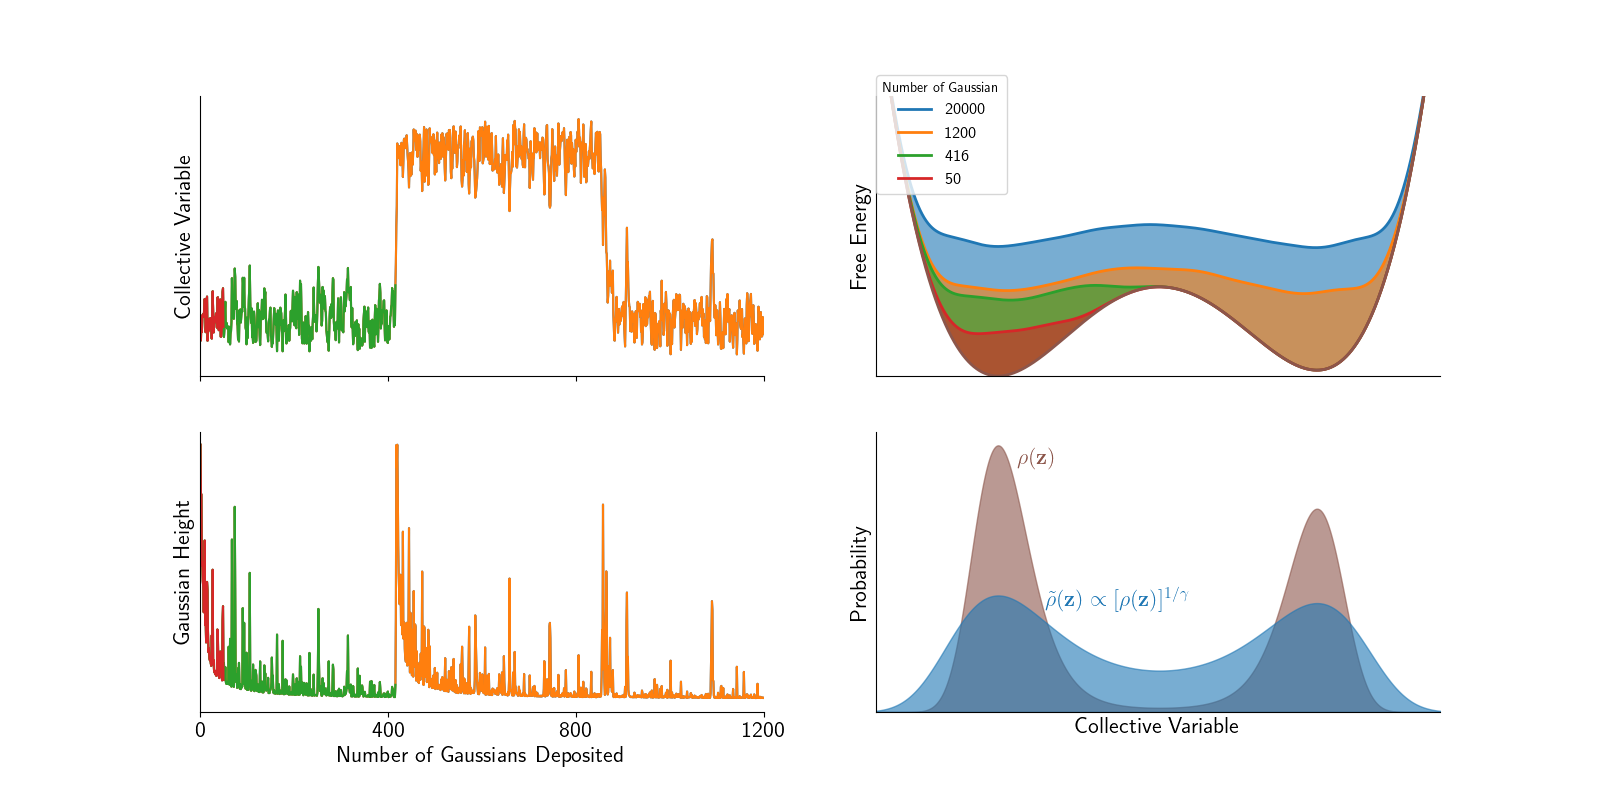
\includegraphics[width=0.95\textwidth]{Figures/MetaD-Figure.png}
    \caption{Prototypical behaviour of a well-tempered metadynamics simulations. Shown are results for a model energy landscape given by $A(z)=2z^4-8z^2+0.1918z$ where the metadynamics simulation is performed using $\beta=0.5$ and $\gamma=4$.
    \textbf{(Left top panel)} Time series of the added Gaussian kernels \textbf{(Left bottom panel)}. The height $H_{k}$ of the added Gaussians goes down as the simulations proceeds (see equations~\ref{wtmetad_update} and~\ref{wtmetad_sum}). \textbf{(Right top panel)} The FES $A(z)$ and FES with added bias potential $A(z)+U_{\mathrm{bias}}(z)$ shown for different number of added Gaussians (colors to correspond to the time series on the left side). The bias potential only partially cancel out the FES at convergence, leading to sampling on an effective FES $A_{\gamma}(\vz) = A(\vz) + U_{\mathrm{bias}}(\vz) =  \frac{1}{\gamma} A(\vz)$ where the barriers have been reduced by a factor of $\gamma$. \textbf{(Right bottom panel)} At convergence, the CV are sampled according to the well-tempered distribution where fluctuations are enhanced as compared to the unbiased distribution (see Equation~\ref{eq:wtmetad_wtdist}). The bias factor $\gamma$ determines how much we enhance the fluctuations. The figure is inspired by Figure~1 in Ref~\cite{Bussi2020}}
    \label{fig:MetaD}
\end{figure*}


%See practical reviews~\cite{10.1002/9781118889886.ch1,10.1007/978-1-4939-9608-7_21} and tutorials~\cite{plumed_masterclass} for guidelines about selecting values for the bias factor $\gamma$, the height $H_{0}$, and the standard deviations $\boldsymbol{\sigma}$.

In between bias potentials updates, after depositing $n$ Gaussian kernels, the bias potential is given by
\begin{align}
\label{wtmetad_sum}
U^{\mathrm{bias}}(\vz,t) &=
\sum_{k=1}^{n}
\exp \left[-\frac{1}{\gamma-1} \beta  U^{\mathrm{bias}}_{k-1}(\vz_k)\right]
G(\vz,\vz_{k})
\nonumber
\\
& =
\sum_{k=1}^{n}
H_{k} \,
\exp \left[-\frac{1}{2}\sum^{d}_{i=1} \frac{(z_i-z_{k,i})^2}{\sigma^2_i} \right]
\end{align}
where we write $H_{k} = H_{0} \, \exp \left[-\frac{1}{\gamma-1} \beta U^{\mathrm{bias}}_{k-1}(\vz_k)\right]$ as the height of the $k$-th added Gaussian.
In the long time limit, the height $H_k$ goes to zero as the scaling factor $\exp \left[-\frac{1}{\gamma-1} \beta U^{\mathrm{bias}}_{k-1}(\vz_k)   \right]$ decreases as $\frac{1}{k}$~\cite{Barducci-PRL-2008,Dama-PRL-2014}. Therefore, as the metadynamics simulations progresses, the change of the bias potential is smaller and it becomes quasi-stationary.
It has been proven~\cite{Dama-PRL-2014} that updating the bias potential according to Equation~\ref{wtmetad_update} leads to an asymptotic solution given by
\begin{equation}
\label{eq:wtmetad_asymptotic}
U^{\mathrm{bias}}(\vz,t \to \infty) = - \left(1-\frac{1}{\gamma} \right)
A(\vz) + c(t)
\end{equation}
where
\begin{equation}
\label{wtmetad_coft}
c(t) = \frac{1}{\beta} \ln
\frac
{\int e^{-\beta A(\vz)} \,  d\vz }
{\int e^{-\beta \left[ A(\vz) + U^{\mathrm{bias}}(\vz) \right]} \, d\vz }
\end{equation}
is a time-dependent constant~\cite{tiwary_rewt}. Note that in the metadynamics literature, the \hyperlink{ref:FES} {FES} is generally denoted as $F(\vz)$ (or $F(\mathbf{s})$) instead of $A(\vz)$.


The bias potential in Equation~\ref{eq:wtmetad_asymptotic} only partially cancels out the \hyperlink{ref:FES} {FES} and the \hyperlink{ref:CV} {CV}s  are sampled according to a so-called well-tempered distribution
\begin{equation}
\label{eq:wtmetad_wtdist}
\tilde{\rho}(\vz) =
\frac
{[\rho(\vz)]^{1/\gamma}}
{\int [\rho(\vz)]^{1/\gamma} d\vz},
\end{equation}
which can be viewed as a distribution where \hyperlink{ref:CV} {CV} fluctuations are enhanced as compared to the equilibrium distribution, see Figure~\ref{fig:MetaD}. The bias factor determines the magnitude of the fluctuation enhancements and also how fast the height $H_{k}$ of the deposited Gaussian kernels goes to zero.

By taking the logarithm on both sides of Equation~\ref{eq:wtmetad_wtdist}, we can view the well-tempered distribution as sampling an effective \hyperlink{ref:FES} {FES},  $A_{\gamma}(\vz) = \frac{1}{\gamma} A(\vz)$, where the barriers have been reduced by a value corresponding to the selected bias factor, as we can see in Figure~\ref{fig:MetaD}. This gives a rule of thumb for selecting the bias factor. It should be chosen such that the barriers become on the order of the thermal energy so that the system can easily migrate between metastable states on the simulation timescale.

In the metadynamics literature, a temperature parameter $\Delta T$ is often used instead of the bias factor $\gamma$. This introduces another interpretation of well-tempered metadynamics. We can view the distribution in Equation~\ref{eq:wtmetad_wtdist} as sampling the \hyperlink{ref:CV} {CV}s at a higher temperature $T+\Delta T$. The bias factor is the ratio of the \hyperlink{ref:CV} {CV} temperature and the simulation temperature, $\gamma = (T + \Delta T)/T$.

Like most \hyperlink{ref:CV} {CV}-based enhanced sampling methods, metadynamics cannot work with too many \hyperlink{ref:CV} {CV}s. In practical applications, we are generally limited to biasing three to four \hyperlink{ref:CV} {CV}s. However, there are variants of metadynamics that allow us to employ a large number of \hyperlink{ref:CV} {CV}s, see Sections~\ref{sec:pb-metad} and~\ref{sec:be-metad}.

\subsubsection{Obtaining the Free Energy Surface}
\label{sec:metad_obtaining_fes}

The \hyperlink{ref:FES} {FES} can be estimated directly from the bias potential through Equation~\ref{eq:wtmetad_asymptotic} by summing up the deposited Gaussians
\begin{align}
\label{eq:metad_sumhills}
A(\vz) &=
- \left(\frac{\gamma}{\gamma-1}\right) U^{\mathrm{bias}}(\vz,t) + K(t)
\nonumber \\
& =
- \left(\frac{\gamma}{\gamma-1}\right)
\sum_{k=1}^{n}
H_{k} \,
\exp \left[-\frac{1}{2}\sum^{d}_{i=1} \frac{(z_i-z_{k,i})^2}{\sigma^2_i} \right] + K(t),
\end{align}
where $K(t)$ is a time-dependent constant that be calculated as described in Refs~\cite{tiwary_rewt,Valsson2016_ARPC_MetaD} and allows us to assess the \hyperlink{ref:FES} {FES}'s convergence and measure error bars. Alternately, a common procedure to assess convergence is to compare \hyperlink{ref:FES} {FES}s obtained at different times by aligning their minimum to zero.

We can also obtain the \hyperlink{ref:FES} {FES} via various post-processing \hyperlink{ref:Reweighting} {reweighting} procedures~\cite{bonomi_rewt,tiwary_rewt,Branduardi-JCTC-2012,Schafer_RewMetaD_2020,Giberti_IterRew_JCTC2019,10.1063/1.5123498,10.1016/j.cplett.2020.137384}.

The most common way to achieve this task is the so-called $c(t)$ reweighting procedure~\cite{bonomi_rewt,tiwary_rewt} that takes the time-dependence of the bias potential into account. The biased configurational distribution at time $t$ is given by
\begin{equation}
\tilde{\nu}(\vx) = \nu(\vx) \, \exp
\left(-\beta\left[
U^{\mathrm{bias}}(\xi(\vx),t)-c(t)
\right] \right)
\end{equation}
where $c(t)$ is a time-dependent constant given by Equation~\ref{wtmetad_coft}. In practise, $c(t)$ can be estimated using
\begin{equation}
c(t) = \frac{1}{\beta} \ln
\frac
{\int \exp \left[ \frac{\gamma}{\gamma-1} \beta U^{\mathrm{bias}}(\vz,t)  \right] d\vz }
{\int \exp \left[ \frac{1}{\gamma-1} \beta U^{\mathrm{bias}}(\vz,t)  \right] d\vz },
\end{equation}
that is obtained by inserting Equation~\ref{eq:wtmetad_asymptotic} into Equation~\ref{wtmetad_coft}~\cite{tiwary_rewt,Valsson2016_ARPC_MetaD}. This relation allows us to reweight and calculate any average of an observable as
\begin{equation}
\label{wtmetad_reweighting}
\langle O(\vx) \rangle = \frac{\langle O(\vx)
\,
e^{
\beta\left[
U^{\mathrm{bias}}(\xi(\vx),t)-c(t)
\right]}\rangle_{\tilde U}}
{\left\langle
e^{\beta \left[
U^{\mathrm{bias}}(\xi(\vx),t)-c(t)
\right]} \right\rangle_{\tilde U}}.
\end{equation}
This \hyperlink{ref:Reweighting} {reweighting} procedure assumes a quasi-stationary bias potential and thus is valid after a short initial transient.

Another \hyperlink{ref:Reweighting} {reweighting} procedure that avoids the calculation of the time-dependent constant $c(t)$ is the so-called last bias \hyperlink{ref:Reweighting} {reweighting}~\cite{Branduardi-JCTC-2012}. In this case, we use weights obtained using the bias potential at the end of the simulation, in other words, the last bias potential. An average of an observable is then calculated as
\begin{equation}
\label{wtmetad_reweighting_lastbias}
\langle O(\vx) \rangle = \frac{\langle O(\vx)
\,
e^{
\beta
U^{\mathrm{bias}}(\xi(\vx),t_F)
}\rangle_{\tilde U}}
{\langle
e^{\beta
U^{\mathrm{bias}}(\xi(\vx),t_F)
} \rangle_{\tilde U}},
\end{equation}
where $t_F$ is the time at the end of the simulation.

Using $O(\vx) = \delta[\vz-\xi(\vx)]$ in Equation~\ref{wtmetad_reweighting} or~\ref{wtmetad_reweighting_lastbias}, allows us to use \hyperlink{ref:Reweighting} {reweighting} to estimate the \hyperlink{ref:FES} {FES} as a function of the biased \hyperlink{ref:CV} {CV}s, or for any other set of \hyperlink{ref:CV} {CV}s. It is a good practice to compare the \hyperlink{ref:FES} {FES} estimated from the bias potential via Equation~\ref{eq:metad_sumhills} to the \hyperlink{ref:FES} {FES} estimated using \hyperlink{ref:Reweighting} {reweighting}. They should give the same results and a major disagreement would indicate that the simulation is not converged or that the \hyperlink{ref:CV} {CV}s might not be good enough. Furthermore, we can estimate error bars for reweighted \hyperlink{ref:FES} {FES}s using block averaging (see PLUMED tutorials~\cite{plumed_masterclass}).

Other post-processing methods for obtaining the \hyperlink{ref:FES} {FES} include mean force integration~\cite{10.1063/1.5123498} and a weighted histogram analysis method~\cite{10.1016/j.cplett.2020.137384}, which both allow for estimating the \hyperlink{ref:FES} {FES} by combining different independent metadynamics simulations. Metadynamics has also been combined with Gaussian Process Regression for obtaining the \hyperlink{ref:FES} {FES}~\cite{Mones2016}.


\subsubsection{Conventional Metadynamics}
\label{sec:meta-classic}

In conventional (non-well-tempered) metadynamics~\cite{Laio-PNAS-2002}, which is the original formulation of metadynamics, the height of Gaussian kernels is kept fixed throughout the simulations. We can view this as the limit $
\gamma \to \infty$ for well-tempered metadynamics. At convergence, this leads to a bias potential that oscillates around the negative of the \hyperlink{ref:FES} {FES}. Thus, on average the bias potentials cancels out the \hyperlink{ref:FES} {FES} and a uniform \hyperlink{ref:CV} {CV} sampling is obtained. In this case, the \hyperlink{ref:FES} {FES} should be estimated as a time-average of the bias potentials~\cite{BussiLaio_ReviewMetaD_2020}
\begin{equation}
A(\vz) = - \frac{1}{n-n_0} \sum^{n}_{k=n_0} U^{\mathrm{bias}}_k(\vz).
\end{equation}
The accuracy of this estimate will depend on how well the biased \hyperlink{ref:CV} {CV}s are \hyperlink{ref:AdiabaticDyn} {adiabatically} separated from the dynamics of the other variables~\cite{laio-gervasio-08,jourdain-lelievre-zitt-21}, see Ref~\cite{BussiLaio_ReviewMetaD_2020} for further discussion regarding this point.

In conventional metadynamics simulations, it is a common practise to introduce restraining walls (i.e., bias potential) to avoid exploring unimportant free energy regions. This is generally not needed in well-tempered metadynamics simulations as the bias factor and the well-tempered distribution naturally limits the extent of CV space exploration.

\subsubsection{Multiple Walkers Metadynamics}
A way to reduce the wall-clock time for convergence and make a better usage of modern parallel HPC resources is to employ multiple walkers or replicas~\cite{Raiteri-JPCB-2006}. The walkers collaboratively sample the free energy \hyperlink{ref:FES} {landscape} and share a bias potential that is constructed by considering the Gaussians deposited by all the walkers.
    %
\subsubsection{Well-Tempered Ensemble}
\label{sec:wtensemble}
The well-tempered ensemble~\cite{Bonomi-PRL-2010} is obtained by using the potential energy $U$ as \hyperlink{ref:CV} {CV} within well-tempered metadynamics. In this case, we obtain a statistical ensemble defined by $\tilde{\rho}(U) \propto [\rho(U)]^{1/\gamma}$ where the potential energy $U$ has the same average as the canonical one but mean square fluctuations amplified by a factor of $\gamma$ (assuming that $\rho(U)$ is roughly Gaussian). By tuning $\gamma$, we can interpolate between the canonical ensemble ($\gamma=1$) and the multicanonical~\cite{Berg1992_Multicanonical} ensemble ($\gamma \to \infty$). In Section~\ref{sec:pt-wte}, we show how this property of the well-tempered ensemble can be used to our benefit when combined with parallel-tempering (see Section~\ref{sec:generalized-ensemble}). The well-tempered ensemble can also be used to obtain thermodynamic properties like the density of states~\cite{Valsson-JCTC-2013}. It has been shown~\cite{Junghans2014wte-wl} that the well-tempered ensemble can be mathematically related to the Wang-Landau method~\cite{wang-landau:prl:2001:wang-landau} and statistical temperature molecular dynamics~\cite{Kim2006_PRL_STMD}.

\subsubsection{Parallel-Bias Metadynamics}
\label{sec:pb-metad}
Parallel-bias metadynamics~\cite{Pfaendtner2015_pbmetad} allows for biasing a large number of \hyperlink{ref:CV} {CV}s simultaneously. This is done by considering many low-dimensional bias potentials (generally one-dimensional), each biasing a separate \hyperlink{ref:CV} {CV}s, all acting within a single simulation.  The metadynamics bias potential update step is modified to account for the effect of the bias potentials on each other. Thus, the method yields the correct low-dimensional free energy \hyperlink{ref:FES} {profile} for each \hyperlink{ref:CV} {CV}. The method has been extended to bias \hyperlink{ref:CV} {CV} sets where the \hyperlink{ref:CV} {CV}s can be considered identical or indistinguishable~\cite{Prakash2018_pbmetad-families}.


\subsubsection{Infrequent Metadynamics}
Well-tempered metadynamics has been extended for obtaining kinetics of rare events in a so-called infrequent metadynamics method~\cite{Tiwary-PRL-2013}. The idea is to reduce the deposition rate, in other words increase $N_{G}$, the number of simulation steps between depositing Gaussians. In this way, we can avoid putting bias on the transition state. If there is no bias on the transition state, we can rescale the time using the ideas of hyperdynamics~\cite{Voter-PRL-1997} and conformational flooding~\cite{Grubmuller-PRE-1995}. The physical time $t_b$ is obtained by summing up the MD steps and scaling the MD time step $dt$ by the bias acting at each step
\begin{equation}
\label{wtmetad_hyperdynamics}
t_b = \sum_{i} dt \, e^{\beta U^{\mathrm{bias}}(\vz(t_{i}),t_{i})},
\end{equation}
where $t_{i} = i\, dt$. By performing multiple simulations, one can obtain a distribution of escape times from a long-lived metastable state. It is possible to assess the reliability of the kinetics by performing a statistical analysis to test how well the obtained escape time distribution follows the expected time-homogeneous Poisson distribution~\cite{KS_Test_JCTC_2014}. An extension on the idea of infrequent metadynamics is frequency adaptive metadynamics~\cite{Wang2018_FA-MetaD} where the deposition rate is adjusted on the fly during the simulation.

\subsubsection{Adaptive Gaussian Metadynamics}
In the adaptive Gaussian variant~\cite{Branduardi-JCTC-2012}, the shape of the deposited Gaussian biasing kernel is not kept fixed but changes with time and adapts to the features of the underlying \hyperlink{ref:FES} {FES}, by employing an off-diagonal variance matrix that is estimated according to certain rules. Employing adaptive Gaussian can improve the performance in some cases, for example, if the \hyperlink{ref:FES} {FES}'s metastable states differ considerably in their shape, or if the \hyperlink{ref:CV} {CV}s are highly coupled.

\subsubsection{Other Variants of Metadynamics}
\label{sec:metad_variants}
An non-exhaustive list of other extensions and variants of metadynamics that have been introduced throughout the year includes
reconnaissance metadynamics~\cite{10.1073/pnas.1011511107},
$\lambda$-metadynamics~\cite{10.1021/jz200808x},
flux-tempered metadynamics~\cite{Singh-JStatPhys-2011,Singh-JCTC-2012},
path-metadynamics~\cite{10.1103/physrevlett.109.020601,10.1063/1.5027392},
funnel metadynamics~\cite{10.1073/pnas.1303186110,10.1038/s41596-020-0342-4},
algorithms for boundary corrections~\cite{McGovern-JCP-2013},
transition-tempered metadynamics~\cite{Dama-JCTC-2014}, metabasin metadynamics~\cite{10.1021/acs.jctc.5b00907},
experiment directed metadynamics~\cite{White_EDM_2015}
ensemble-biased metadynamics~\cite{Marinelli_EnsembleBiased_2015},
target metadynamics~\cite{GilLey_TargetMetaD_2016},
$\mu$-tempered metadynamics~\cite{10.1063/1.4937939},
adaptive-numerical-bias metadynamics~\cite{10.1002/jcc.25066},
altruistic metadynamics~\cite{10.1021/acs.jpcb.6b00087,10.1063/1.4978939},
metadynamics for automatic sampling of quantum property manifolds~\cite{Lindner_ASQPM-MetaD_2019},
and
metadynamics with scaled hypersphere search for high-dimensional FES~\cite{Mitsuta_SHS-MetaD_JCTC2020}.
We refer the reader to the references for further details. Metadynamics has also been used in various types of hybrid methods as discussed in Section~\ref{sec:hybrids}.

\subsubsection{Public Implementations of Metadynamics}
Various variants of metadynamics are implemented in the PLUMED 2 enhanced sampling plug-in~\cite{Bonomi-CPC-2009,Tribello2014,plumed-nest}. PLUMED also includes numerous practical tutorials showing how to perform and analyze metadynamics simulations~\cite{plumed_masterclass}.

Metadynamics are also available in the external libraries SSAGES and the Colvars module, and also is natively implemented in some MD codes codes such as CP2K and DESMOND, see Table 2 in Ref~\cite{BussiLaio_ReviewMetaD_2020}.

\subsection{Variationally Enhanced Sampling}
\label{sec:ves}
A more recently introduced ABP method is variationally enhanced
sampling~\cite{Valsson_VES_PRL_2014,Valsson2020Handbook_VES} that is based on a variational principle.
In variationally enhanced sampling, a bias potential $U^{\mathrm{bias}}(\vz)$ is constructed by minimizing a convex functional given by
\begin{equation}
\label{ves_omega}
\Omega [U^{\mathrm{bias}}] =
\frac{1}{\beta} \ln
\frac
{\int e^{-\beta \left[ A(\vz) + U^{\mathrm{bias}}(\vz)\right]} \, d\vz }
{\int e^{-\beta A(\vz)} \, d\vz}
+
\int p_{\mathrm{tg}}(\vz) \, U^{\mathrm{bias}}(\vz) \, d\vz,
\end{equation}
where $p_{\mathrm{tg}}(\vz)$ is a so-called \hyperlink{ref:targetdist}{target distribution} that is chosen by the user. The $\Omega [U^{\mathrm{bias}}]$ functional has a global minimum given by
\begin{equation}
\label{ves_biaspotential}
U^{\mathrm{bias}}(\vz) = -A(\vz)- \frac{1}{\beta} \ln {p_{\mathrm{tg}}(\vz)} + C,
\end{equation}
where $C$ is an unimportant constant. This bias potential results in a biased \hyperlink{ref:CV} {CV} distribution that is equal to the \hyperlink{ref:targetdist}{target distribution}, $\tilde{\rho}(\vz) = p_{\mathrm{tg}}(\vz)$. Therefore, the \hyperlink{ref:targetdist}{target distribution} determines the \hyperlink{ref:CV} {CV} sampling that is obtained when minimizing $\Omega [U^{\mathrm{bias}}]$. By choosing a \hyperlink{ref:targetdist}{target distribution} that is easier to sample than the equilibrium distribution, we enhance the sampling. Furthermore, we can directly obtain the \hyperlink{ref:FES} {FES} from the bias potential through Equation~\ref{ves_biaspotential}.

To obtain a better understanding of the functional in Equation~\ref{ves_omega}, we can rewrite it as~\cite{Valsson2020Handbook_VES,Invernizzi-PNAS-2017}
\begin{equation}
\beta \Omega [U^{\mathrm{bias}}] = D_{\mathrm{KL}}(p_{\mathrm{tg}}||\tilde{\rho})-D_{\mathrm{KL}}(p_{\mathrm{tg}}||\rho),
\end{equation}
where $D_{\mathrm{KL}}(p||q)=\int p(\vx) \ln\frac{p(\vx)}{q(\vx)} \, d\vx$ is the Kullback-Leibler divergence from probability distribution $p(\vx)$ to probability distribution $q(\vx)$. Therefore, minimizing $\Omega [U^{\mathrm{bias}}]$ is equivalent to minimizing the Kullback-Leibler divergence (or the relative entropy or cross entropy) between the \hyperlink{ref:targetdist}{target distribution} $p_{\mathrm{tg}}(\vz)$ and the biased distribution $\tilde{\rho}(\vz)$~\cite{Rubinstein-MetCompAppProb-1999,Shell-JCP-2008,Bilionis-JCompPhys-2012,Zhang_SIAM-JSC-2014}.

In practice, $\Omega [U^{\mathrm{bias}}]$ is minimized by introducing a functional form for the bias potential $U^\mathrm{bias}(\vz,\boldsymbol{\alpha})$ that depends on a set of variational parameters $\boldsymbol{\alpha}$. We then go from an abstract functional minimization to a minimization of the multidimensional function $\Omega(\boldsymbol{\alpha}) = \Omega [U^{\mathrm{bias}}(\boldsymbol{\alpha})]$. The elements of the gradient $\nabla \Omega(\boldsymbol{\alpha})$ are defined as
\begin{equation}
\frac
{\partial \Omega(\boldsymbol{\alpha})}
{\partial \alpha_{i}}
 = -
\left<
\frac
{\partial U^{\mathrm{bias}}(\vz;\boldsymbol{\alpha})}
{\partial \alpha_{i}}
\right>_{\tilde{U}(\boldsymbol{\alpha})}
+
\left<
\frac
{\partial U^{\mathrm{bias}}(\vz;\boldsymbol{\alpha})}
{\partial \alpha_{i}}
\right>_{p}.
\end{equation}
The first term is an ensemble average obtained in the biased ensemble given by the
\hyperlink{ref:biasingE}{biased potential energy} $\tilde{U}(\vx;\boldsymbol{\alpha}) = U(\vx) + U^{\mathrm{bias}}(\xi(\vx);\boldsymbol{\alpha})$, and the second term is an average over the \hyperlink{ref:targetdist}{target distribution}.  The gradient is noisy due to the need of estimating the first term from a biased simulation. Therefore, it is better to employ stochastic optimization methods to minimize $\Omega(\boldsymbol{\alpha})$ by updating the bias potential iteratively.

The most general bias representation is to use a linear expansion in some set of basis function
\begin{equation}
U^{\mathrm{bias}}(\vz;\boldsymbol{\alpha}) = \sum_{\mathbf{k}} \alpha_{\mathbf{k}} \cdot f_{\mathbf{k}}(\vz).
\end{equation}
This could for example be a tensor product of one-dimensional basis functions like Chebyshev or Legendre polynomials, or wavelets. In particular, localized wavelet basis functions have been shown to perform the best~\cite{ValssonPampel_Wavelets_2022}. A neural network bias potential has also been used~\cite{Bonati2019_NN-VES}. Furthermore, one can use bespoke bias potentials like a model of the free energy \hyperlink{ref:FES} {profile}~\cite{McCarty2016_JCTC,Piaggi2016_Faraday}.

The \hyperlink{ref:targetdist}{target distribution} $p_{\mathrm{tg}}(\vz)$ can be chosen freely by the user. However, one needs to keep in mind that it should be chosen such that the sampling is easier than in the equilibrium distribution. The most straightforward choice would be a uniform \hyperlink{ref:targetdist}{target distribution}, such that the aim to completely cancel out the \hyperlink{ref:FES} {FES} and flatten the sampling in the \hyperlink{ref:CV} {CV} space. However, that is generally not optimal. Instead it is better to only enhance \hyperlink{ref:CV} {CV} fluctuations to a certain degree and thus only partly cancel out the \hyperlink{ref:FES} {FES}~\cite{Valsson-JCTC-2015}. We can achieve this by employing a well-tempered distribution as in Equation~\ref{eq:wtmetad_wtdist} (see Figure~\ref{fig:MetaD}). The bias factor $\gamma$ determines how much we enhance \hyperlink{ref:CV} {CV} fluctuations. The well-tempered distribution is unknown \textit{a priori} so it needs be determined iteratively~\cite{Valsson-JCTC-2015}.

The \hyperlink{ref:FES} {FES} can be estimated directly from the bias potential though Equation~\ref{ves_biaspotential}. Furthermore, the \hyperlink{ref:FES} {FES}, both for the biased \hyperlink{ref:CV} {CV}s and for any other \hyperlink{ref:CV} {CV}s, can be obtained through \hyperlink{ref:Reweighting} {reweighting}, where we can also estimate error bars. Note that  in variationally enhanced sampling, we generally do not need to account for time-dependent constants as in metadynamics. It is sufficient to include the bias potential in the weight when performing the reweighting procedure. As for metadynamics, it is a good practise to estimate the \hyperlink{ref:FES} {FES} both from the bias potential and through \hyperlink{ref:Reweighting} {reweighting} and compare the results. Furthermore, in cases where the bias potential might not have sufficient variational flexibility to represent the underlying \hyperlink{ref:FES} {FES}, the reweighted results can be more accurate.

Variationally enhanced sampling has been extended to obtaining kinetics of rare events~\cite{McCarty-PRL-2015}, using the same principles as used in infrequent metadynamics. The idea is to use variationally enhanced sampling to construct a bias potential that only floods the \hyperlink{ref:FES} {FES} up to some given cutoff value. If the flooding bias potential does not touch the transition state, we can rescale the biased simulation times using Equation~\ref{wtmetad_hyperdynamics} as in infrequent metadynamics. It is convenient and useful to combine the flooding bias potential with infrequent metadynamics as done in Ref~\cite{Palazzesi2017_JPCL}.

Furthermore, variationally enhanced sampling has been extended in various ways, for example:
to obtain parameters for phenomenological coarse-grained model~\cite{Invernizzi-PNAS-2017};
to perform Monte Carlo renormalization group simulations~\cite{Wu_VES-RGMC_PRL2017,Wu_VES-RGMC_PRE2019,Wu_VES-RGMC_PRL2020};
to perform multithermal-multibaric simulations~\cite{Piaggi_MultiVES_2019};
for enhanced sampling targeting transistion states~\cite{Debnath_VES-TS_2019}; and
multiscale simulations for sub-optimal CVs~\cite{Invernizzi_VES_DelteF_2019}.

Variationally enhanced sampling is implemented in the VES Code module of PLUMED 2. The VES Code also includes practical tutorials showing how to employ the method.




\subsection{Adaptive Biasing Force}
\label{sec:ABF}

\begin{figure}
    \centering
    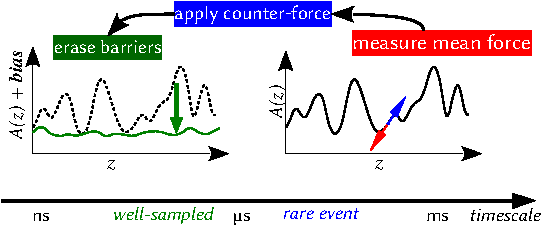
\includegraphics{Figures/abf_new.pdf}
    \caption{Principle of the ABF method. The native free energy surface (solid black line, right) shows high barriers, resulting in long transition time scales.
    In ABF the mean force (red arrow) is measured and countered by the biasing force (blue arrow). As a result, the biased free energy surface (dashed black line, left) approaches a uniform one, and the transition time scales become short enough to be well-sampled in simulations.}
    \label{fig:ABF}
\end{figure}

The \hyperlink{ref:Adaptive} {adaptive} Biasing Force method (ABF) is rooted in free energy estimation by thermodynamic integration (Section~\ref{sec:fe_estimators:TI}).
In ABF, the gradient of the free energy with respect to selected \hyperlink{ref:CV} {CV}s $\vz = \xi(\vx)$ is estimated, and that estimate is used to apply a time-dependent external force $\vF^\mathrm{ABF}_t(\vz)$ that counteracts the estimated free energy gradient, enhancing sampling along those coordinates.

The principle is the following:
\begin{enumerate}
 \item A small number of slow degrees of freedom $\vz=\xi(\vx)$  are chosen.
 \item In the simulation, the gradient of the free energy \hyperlink{ref:FES} {surface} $A(\vz)$  is estimated as:
\begin{equation}
    \nabla_\vz A(\vz) = - \left\langle \vF_\xi(\vx)  \right\rangle_{\xi(\vx) = \vz}
\end{equation}
That is, as the conditional ensemble average of a collective force $\vF_\xi(\vx)$ at a given value of $\xi(\vx)$ .
 \item When sufficient sampling is collected to have a reliable estimate of the average force at the current value of $\vz$, a biasing force $\vF^\mathrm{ABF}_t(\vz)$ equal to the opposite of this average is applied.
 \item This force cancels out, on average, the forces acting along $\vz$, leveling the free energy barriers and accelerating diffusion in \hyperlink{ref:CV} {collective variable} space.
 \item At convergence, the biasing force is the negative of the gradient of the free energy, and $\vz$ experiences a flat effective free energy \hyperlink{ref:FES} {landscape}. The gradient can be integrated numerically to estimate the free energy \hyperlink{ref:FES} {landscape} itself.
\end{enumerate}

Thus the core of ABF is an adaptation method to calculate a time-dependent biasing force $\vF^\mathrm{ABF}_t$ that, at long times, converges towards the free energy gradient $\nabla_\vz A$, or an approximation of it.

The following optional components of an ABF method can be used to obtain reliable free energies:
\begin{enumerate}
\item a different \textit{a posteriori} estimator of the free energy gradient (if the one used in ABF is approximate eg. eABF, gABF, see Sections~\ref{sec:eABF} and \ref{sec:ABF_variants});
\item a method to integrate the free energy gradients and obtain the free energy \hyperlink{ref:FES} {surface}.\cite{Henin2021integration}
\end{enumerate}

In what we will call standard ABF (Section~\ref{sec:ABF_standard}), a single simulation is run at a time and the exact free energy derivative with respect to the coordinate of interest is estimated directly as an ensemble average.
Variants may involve multiple interacting replicas of the simulation, fictitious proxy coordinates, approximate gradient estimators, and additional biasing forces or potentials. ABF methods can be shown to converge quickly to equilibrium for well chosen reaction coordinates, see for example the following mathematical analysis for rigorous formulations~\cite{lelievre-rousset-stoltz-08,benaim-brehier-monmarche-20}.

\subsubsection{Standard ABF}
\label{sec:ABF_standard}
In the original formulation of ABF\cite{Darve2000, Darve2001, Darve2002}, the collective force is calculated based on a constraint force calculation. That is, a constraint solver algorithm such as SHAKE or RATTLE\cite{Ryckaert1977,Andersen1983} is executed as if to keep the coordinate of choice constant.
However, the calculated constraint force is not applied and the coordinate remains unconstrained; instead, this force is used to determine the collective force $\vF_\xi$, which is averaged over time to estimate the free energy derivative.\cite{Darve2001}
Whereas a usual constraint algorithm would cancel the \textbf{instantaneous} collective force acting on the coordinate, the ABF algorithm cancels the ensemble average of this force, so that the coordinate ``sees'' no force \textbf{on average}, but simply zero-mean fluctuations. This is equivalent to evolving on a locally flat free energy \hyperlink{ref:FES} {surface}.


An alternate formulation that does not need an iterative constraint solver was proposed,\cite{Henin2004} using a projection of Cartesian forces.\cite{denOtter2000} This was the basis of the first public implementation of ABF in NAMD.
These were completed with vector formulations that allow for estimation of free energy gradients along several \hyperlink{ref:CV} {collective variable}s, either using time derivatives\cite{Darve2008}, or projected forces.\cite{Henin2010a}
The latter is implemented in the Colvars Module.\cite{Fiorin2013}

In the multidimensional projected force version,\cite{Henin2010a} the instantaneous collective force is estimated as:\cite{Ciccotti2005}
\begin{equation}
\vF_\xi(\vx) = - \vv_i(\vx) \cdot \nabla U(\vx) + \beta^{-1} \nabla \cdot \vv_i(\vx)
\end{equation}
where $\vv_i$ is a vector field associated to each coordinate $\xi_i$, verifying for all $i,j$:
\begin{equation}
    \vv_i \cdot \nabla \xi_j = \delta_{i,j}
\end{equation}

% $\vv_i$ plays the same role as $\frac{\partial \vx}{\partial z_i}$ if a coordinate transform from Cartesian to generalized coordinates was defined.\cite{Comer2015}

In dimension greater than 1, obtaining the free energy \hyperlink{ref:FES} {surface} knowing an estimate of its gradients is not trivial.
In the Colvars implementation, this is done by solving a Poisson equation\cite{Lelievre2010, Alrachid2015, Henin2021integration}.

For a detailed review of ABF, see Ref~\cite{Comer2015}.

Variants of ABF have been proposed that differ from the original approach in several respects.
This includes the use of multiple replicas of the simulation, extended dynamics (fictitious coordinate), other ways to calculate the biasing force (pABF, ABF-FUNN), and combination of ABF dynamics with other biases.
Variants that combine ABF with other sampling methods are presented in Section~\ref{sec:abf_hybrids}.

\subsubsection{Multiple-Walker ABF}
\label{sec:mwABF}

In shared or multiple-walker ABF (mwABF),\cite{Lelievre2007, Minoukadeh2010, Comer2014mwABF} several ABF simulations of the same system using the same \hyperlink{ref:CV} {collective variable} run concurrently, sharing their ABF data at periodic intervals, thus benefiting from the exploration of all other walkers.
In the selection variant,\cite{Minoukadeh2010, Comer2014mwABF} walkers are replicated or killed using a selection criterion that promotes undersampled regions of \hyperlink{ref:CV} {collective variable} space.

\subsubsection{Extended-system ABF}
\label{sec:eABF}

In extended-system ABF (eABF),\cite{Lelievre2010eABF, Zheng2012} the coordinate is not a \hyperlink{ref:CV} {collective variable} $z = \xi(\vx)$, but an additional variable $\lambda$, separate from Cartesian coordinates, so that the dynamics is now propagated in the extended space $(\vx, \lambda)$.
$\lambda$ is coupled to the \hyperlink{ref:CV} {collective variable} by a harmonic restraint: $U^\mathrm{ext}(\vx, \lambda) = 1/2 k (\lambda - \xi(\vx))^2$.
The main benefit of eABF is that the biasing coordinate $\lambda$ is not a function of Cartesian coordinates, so all geometric considerations raised by the projected force formalism become moot. This makes eABF easy to implement for any combination of \hyperlink{ref:CV} {collective variable}s, as long as their gradients can be calculated.
One limitation is that the free energy associated to $\lambda$ is close to, but not identical to that associated to $z$, which is the quantity of interest.
The implementation of eABF in the Colvars Module\cite{Lesage2017} is complemented by two the \hyperlink{ref:FEestimator} {free energy estimator}, CZAR\cite{Lesage2017} and an Umbrella Integration estimator.\cite{Kastner2005, Zheng2012, Fu2016}


\subsubsection{Other ways to calculate the biasing force}
\label{sec:ABF_variants}

Besides the classic ways mentioned above (constraint force, force projection, time derivatives, eABF), other estimators have been proposed:
\begin{enumerate}
\item by projection of the (noisy) gradient estimate on the space of ``true gradients" to reduce their variance: projected ABF (pABF)\cite{lelievre-rousset-stoltz-07-a,Alrachid2015}
\item by ABF with Gaussian Process Regression\cite{Mones2016}
\item by a neural network (ABF-FUNN)\cite{Guo2018}
\item using an implicit, adiabatic extended coordinate: ABF with adiabatic \hyperlink{ref:Reweighting} {reweighting} (ABF-AR)\cite{Cao2014}
\item approximated as the sum of independent biasing forces on individual \hyperlink{ref:CV} {collective variable}s: generalized ABF (gABF)\cite{Chipot2011, Zhao2017}.
\end{enumerate}


\subsubsection{Public implementations of ABF}

The first public implementation of ABF\cite{Henin2004} was a scripted extension to NAMD.\cite{Phillips2020}
This was superseded by a more flexible, multi-dimensional implementation\cite{Henin2010a} which is part of the Collective Variables (Colvars) Module \cite{Fiorin2013}.
The Colvars Module is interfaced with NAMD\cite{Phillips2020}, LAMMPS\cite{Plimpton1995}, Gromacs\cite{Abraham2015}, and VMD\cite{Humphrey1996} for colvar analysis \cite{Henin2022dashboard}.
An interface of the Colvars Module with Tinker-HP\cite{Lagardere2018} is in preparation.
ABF is implemented in PMFlib\cite{kulhanek2011pmflib} for use in the sander version of AMBER.
Dynamic Reference Restraining\cite{Zheng2012} (equivalent to eABF) is implemented in PLUMED.\cite{Tribello2014}
ABF-FUNN is part of SSAGES.\cite{Sidky2018}


\subsection{Adaptive Biasing Potential Methods Using the Potential Energy as a Collective Variable}
\label{sec:abp_energy}

A certain class of enhanced sampling methods can be loosely defined as adaptive biasing potential methods using the potential energy $U$ as a CV though they might not be explicitly formulated in terms of a bias potential. What unites these methods is that they aim to sample a potential energy distribution $p_{\mathrm{tg}}(U)$ (i.e., a target potential energy distribution) that is broadened or expanded as compared to unbiased distribution corresponding to the simulation temperature. Thus, they can be considered as sampling from a ensemble where the sampling should be easier\footnote{sometimes called a generalized ensemble in the literature, see the following Section~\ref{sec:generalized-ensemble} for a more broader discussion of this idea.}. A well known example of this is the multicanonical (or multithermal) ensemble where the aim to sample the potential energy near uniformly in a given range. The idea can also be extended to multithermal-multibaric simulations by incorporating the volume as a variable whose dynamics is biased or modified~\cite{Okumura_MultiTP_2004,Shell_MultiTP_2002}. Furthermore, sometime only a subset of the potential energy is used to better focus the sampling enhancement~\cite{Yang_SITS_2009}.

Methods in this category include for example
the multicanonical ensemble~\cite{Berg1992_Multicanonical},
Wang-Landau sampling~\cite{wang-landau:prl:2001:wang-landau}\footnote{The Wang-Landau procedure is also used in more general settings for other variables, see Section~\ref{sec:singlestate} for further details},
statistical temperature MD~\cite{Kim2006_PRL_STMD},
metadynamics using the energy as CV~\cite{Micheletti_MetaE_Energy_2004,Bonomi-PRL-2010}
(which is the the well-tempered ensemble discussed in Section~\ref{sec:wtensemble} when using well-tempered metadynamics, see also Ref~\cite{Valsson-JCTC-2013}),
integrated tempering sampling~\cite{Gao_ITS_2008,Gao_ITS_Review_2015}.
Furthermore, variationally enhanced sampling and on-the-fly probability-enhanced sampling have been extended to perform simulations in the multithermal and the multithermal-multibaric ensembles as described in Refs~\citep{Piaggi_MultiVES_2019,Piaggi_MultiVES+CV_2019} and~\citep{invernizzi2020unified}, respectively.

To achieve the given target potential energy distribution $p_{\mathrm{tg}}(U)$, these methods employ some kind of adaptive or iterative scheme to estimate \textit{a priori} unknown quantities. For example, this can be the density of states~\cite{wang-landau:prl:2001:wang-landau,Kim2006_PRL_STMD,DePablo_DOS_2012}, factors or weights in sum over Boltzmann factors at different temperatures~\cite{Gao_ITS_2008,invernizzi2020unified}, or a free energy as in the case of the well-tempered metadynamics. As said above, these methods are not necessarily explicitly formulated in terms of a bias potential. Nevertheless, we can still associate an effective bias potential as function of the potential energy to them
\begin{equation}
U_\mathrm{bias}(U) = - A(U) -\frac{1}{\beta} \ln p_{\mathrm{tg}}(U) = - U + \frac{1}{\beta} \ln \Omega(U) -\frac{1}{\beta} \ln p_{\mathrm{tg}}(U),
\end{equation}
where $\Omega(U) = \int d\vx \, \delta(U-U(\vx))$ is the density of states, and we ignore unimportant constants. Therefore, we can loosely define these methods as adaptive biasing potential methods using the potential energy $U$ as a CV. From this equation, we can also see a certain theoretical equivalence between methods that work with the density of states, such as Wang-Landau sampling and statistical temperature MD, and methods that work with the free energy, such as metadynamics, see Ref~\cite{Junghans2014wte-wl} for further discussion on this point.

\section{Generalized ensemble and replica exchange methods}
\label{sec:generalized-ensemble}

A broad category of simulation methodologies known as \emph{generalized ensemble}~\cite{okamoto:biopolymers:2001:generalized-ensemble} (also sometimes referred to \emph{extended ensemble}~\cite{iba:intl-j-mod-phys-c:2001:extended-ensemble}) algorithms have become popular over the last two decades.
The main  algorithmic classes in this category are \hyperlink{ref:ReplEx} {replica exchange},~\cite{geyer:conference-proceedings:1991:replica-exchange} which includes parallel tempering~\cite{hukushima-nemoto:j-phys-soc-jpn:1996:parallel-tempering,hansmann:chem-phys-lett:1997:parallel-tempering-monte-carlo,sugita-okamoto:chem-phys-lett:1999:parallel-tempering-md} and Hamiltonian exchange~\cite{sugita-kitao-okamoto:jcp:2000:hamiltonian-exchange,fukunishi-watanabe-takada:jcp:2002:hamiltonian-exchange,jang-shin-pak:prl:2003:hamiltonian-exchange,kwak-hansmann:prl:2005:hamiltonian-exchange}, among others, and the serial equivalent, the method of \hyperlink{ref:ExpEns} {expanded ensemble}s~\cite{lyubartsev:jcp:1992:expanded-ensembles}, which includes simulated tempering~\cite{marinari-parisi:europhys-lett:1992:simulated-tempering,geyer-thompson:j-am-stat-assoc:1995:expanded-ensembles} and simulated scaling~\cite{li-fajer-yang:jcp:2007:simulated-scaling}.

In both replica exchange and expanded ensemble algorithms, a mixture of thermodynamic states are sampled within the same simulation framework. Simulations are able to access all of the  thermodynamic states through a stochastic hopping process between these thermodynamic states.  In the rest of the discussion of both replica exchange and expanded ensembles, we will often use ``states" as shorthand for thermodynamically defined macrostates, which all share the same configuration space $\Sigma$, but each of which have different probabilities due to the differences in $T$, $p$, or Hamiltonian parameters.

In \hyperlink{ref:ExpEns} {expanded ensemble} simulations, the states are explored in a single simulation via a biased random walk in state space; in \hyperlink{ref:RepEx} {replica exchange} simulations, multiple coupled simulations are carried out in parallel, and periodically the simulations exchange thermodynamic states with each other, keeping the same number of simulations at each state. Both methods, if implemented correctly, and potentially after an initial equilibration stage, allow estimation of equilibrium expectations at each state as well as free energy differences between states.

The primary reason for introducing switching between thermodynamic states is that the transitions between these different thermodynamic states can reduce correlation times in configurational sampling at any given thermodynamic state and increase sampling efficiency relative to straightforward sampling of a single state. This acceleration is because the simulations can ``go around"  kinetic barriers within any of these single states. This is done by escaping to a neighboring state where, by happenstance of the path or better yet by design, the barriers are lower.  For this switching between states to work, each thermodynamic state must have neighbors which have a moderate (perhaps 5-20\%, depending on the method) overlap in the configurational space each samples, and overall state space must be connected, which means that there must exist some pathways between all the states. This class of methods therefore only works when the states are designed to have overlap, such as alchemical intermediates, temperatures, or harmonic biasing potentials, and not when the states are defined by values of a collective variable.

Because of their popularity, these algorithms and their properties have been the subject of intense study over recent years.
For example, given optimal weights, \hyperlink{ref:ExpEns} {expanded ensemble} simulations have been shown to have provably higher exchange acceptance rates than replica exchange simulations using the same set of thermodynamic states~\cite{park:pre:2008:simulated-tempering}.
Higher exchange attempt frequencies have been demonstrated to improve mixing for replica exchange simulations~\cite{sindhikara-meng-roitberg:jcp:2008:exchange-frequency,sindhikara-emerson-roitberg:jctc:2010:exchange-often-and-properly}.
Alternative velocity rescaling schemes have been suggested to improve exchange probabilities~\cite{nadler-hansmann:pre:2007:optimized-replica-exchange-moves}.
Other work has examined the degree to which replica exchange simulations enhance sampling relative to straightforward molecular dynamics simulations~\cite{rhee-pande:biophys-j:2003:multiplexed-replica-exchange,zuckerman-lyman:jctc:2006:replica-exchange-efficiency,gallicchio-levy:pnas:2007:replica-exchange,nymeyer:jctc:2008:replica-exchange-efficiency,tavan:cpl:2008:pseudoconvergence,rosta-hummer:jcp:2009:replica-exchange-efficiency,rosta-hummer:jcp:2010:simulated-tempering-efficiency}.
Numerous studies have examined the issue of how to optimally choose thermodynamic states to enhance sampling in systems with second-order phase transitions~\cite{kofke:2002:jcp:acceptance-probability,katzberger-trebst-huse-troyer:j-stat-mech:2006:feedback-optimized-parallel-tempering,trebst-troyer-hansmann:jcp:2006:optimized-replica-selection,nadler-hansmann:pre:2007:generalized-ensemble,gront-kolinski:j-phys-condens-matter:2007:optimized-replica-selection,park-pande:pre:2007:choosing-weights-simulated-tempering,shenfeld-xu:pre:2009:thermodynamic-length}, though systems with strong first-order-like phase transitions (such as two-state protein systems) remain challenging~\cite{neuhaus-magiera-hansmann:pre:2007:parallel-tempering-first-order,straub:jcp:2010:generalized-replica-exchange}.
A number of combinations~\cite{fenwick-escobedo:jcp:2003:replica-exchange-expanded-ensembles,mitsutake-okamoto:jcp:2004:rest} and elaborations~\cite{mitsutake-sugita-okamoto:2003:remuca,rhee-pande:biophys-j:2003:multiplexed-replica-exchange,simmerling:jctc:2007:reservoir-replica-exchange,gallicchio-levy-parashar:j-comput-chem:2008:asynchronous-replica-exchange,hansmann:physica-a:2010:replica-exchange} of these algorithms have also been explored.
A few publications have examined the mixing and convergence properties of replica exchange and expanded ensemble algorithms with mathematical rigor~\cite{madras-randall:annals-appl-prob:2002:decomposition-theorem,bhatnagar-randall:acm:2004:torpid-mixing,woodard_conditions_2009,woodard_sufficient_2009}, but there remain many unanswered questions about these sampling algorithms, both in terms of theoretical bounds and practical guidelines for how much these methods accelerate sampling for complex molecular systems.

In these methods, we label the different $K$ thermodynamic states either using an \hyperlink{ref:AuxVar} {auxiliary variable} $\mathbf{\lambda}$  or by an index $k$. We will assume that the simulation can visit the same configurations for all each choice of $\mathbf{\lambda}$. \footnote{Note however that the Boltzmann weights of any given sample with coordinates $\vx$ can vary significantly between choices of $\mathbf{\lambda}$. For example, if the $K$ thermodynamic states are defined by different temperatures, then the simulation will visit all of the same sets of configurations, but low-energy configurations will have much higher probability at lower temperatures.} Each choice of $\lambda$ results in a sub-ensemble within this expanded ensemble, in which we can carry out a perfectly reasonable simulation in absence of any switching. Finally, note that in this section, we use \hyperlink{ref:reduced} {reduced} units, as it makes it possible to use a common framework and a coherent notation for the different replica exchange and \hyperlink{ref:ExpEns} {expanded ensemble} methods, easing the comparison between the schemes.

\subsection{Replica exchange}
\label{sec:ReplicaExchange}
In a replica exchange simulation, we consider $K$ simulations, with one simulation in each of the $K$ thermodynamic states.  These states could be simulations at different temperatures or $\lambda$ values, and in many cases the data gathered in all of the states is important to calculate observables. However, in other cases, only one simulation actually samples a state of interest, and the other simulations are added exclusively to aid the sampling in one way or another.

The current state of the replica exchange simulation is given by $(X,S)$, where $X$ is a vector of the configurations of \emph{all} of the replicas, $X \equiv \{\vx_1, \vx_2, \ldots, \vx_K\}$, and $S \equiv\{s_1,\ldots,s_K\} \in \mathcal{S}_K$ is a permutation of the state indices $\{1, \ldots, K\}$ associated with each of the replica configurations $\{\vx_1, \ldots, \vx_K\}$. Then the joint probability density of the entire set of all simulations $\mathcal{Q}$ is defined by
\begin{eqnarray}
\mathcal{Q}(X, S) &\propto& \prod_{i=1}^{K} \mu_{s_i}(\vx_i) \propto \exp\left[-\sum_{i=1}^K u_{s_i}(\vx_i)\right]
\label{eq:parallereplica}
\end{eqnarray}
with the conditional densities given by
\begin{eqnarray}
\mathcal{Q}(X | S) &=& \prod_{i=1}^K \left[ \frac{e^{-u_{s_i}(\vx_i)}}{\int_\Omega dx \, e^{-u_{s_i}(\vx_i)}}\right]
\end{eqnarray}
and
\begin{eqnarray}
\mathcal{Q}(S | X) &=& \frac{\exp\left[- \sum\limits_{i=1}^K u_{s_i}(\vx_i) \right]}{\sum\limits_{S' \in \mathcal{S}_K} \exp\left[- \sum\limits_{i=1}^K u_{s'_i}(\vx_i) \right]}
\end{eqnarray}

In the most standard replica exchange simulation algorithms, an update of the state permutation $S$ of the $(X,S)$ sampler state only considers exchanges between neighboring states~\cite{hukushima-nemoto:j-phys-soc-jpn:1996:parallel-tempering,hansmann:chem-phys-lett:1997:parallel-tempering-monte-carlo,sugita-okamoto:chem-phys-lett:1999:parallel-tempering-md,sugita-kitao-okamoto:jcp:2000:hamiltonian-exchange,fukunishi-watanabe-takada:jcp:2002:hamiltonian-exchange,jang-shin-pak:prl:2003:hamiltonian-exchange,kwak-hansmann:prl:2005:hamiltonian-exchange}.
One such scheme involves attempting to exchange either the set of state index pairs $\{(1,2), (3,4), \ldots\}$ or $\{(2,3), (4,5), \ldots\}$, chosen with equal probability.

%\begin{comment}
%~\footnote{It is again common to consider the set of $K$ states to lie on a torus, such that exchanges of $(K,1)$ are also attempted.}.
%\end{comment}

Each state index pair $(i,j)$ exchange attempt is carried out independently, with the exchange of states $i$ and $j$ associated with configurations $\vx_i$ and $\vx_j$, respectively, accepted with probability
\begin{eqnarray}
\label{eq:re_exchange_prob}
P_\mathrm{accept}(\vx_i, i, \vx_j, j) &=& \min\left\{ 1, \frac{e^{-[u_i(\vx_j)+u_j(\vx_i)]}}{e^{-[u_i(\vx_i) + u_j(\vx_j)]}}\right\}
\label{eq:metropolis-replica}
\end{eqnarray}
using a Metropolis-Hastings criterion.
However, it is also possible to sample from the space of all possible permutations, which can in some cases improve sampling~\cite{shirts_gibbssamp}.

Because replica exchange is so general, only requiring that the $K$ states have the same coordinates but any reasonable reduced potentials $u_i$ that have overlap with each other, then there are many different variants that attempt to solve different sampling problems by defining different $u_i$.

The most straightforward versions are parallel implementations of algorithms that already use $K$ simulations. For example, if one is computing some property as a function of temperature, then one can run a number of simulations at different temperatures, with the simulations at higher temperature providing faster kinetics to all of the simulations. If one is performing an alchemical protein-ligand binding simulation, then one typically has simulations at $K$ values of $\lambda$, which describe the degree of interaction of the ligand with the rest of the system, which can be run in replica exchange. In this case, the fully interacting ligand can escape by moving to the fully uncoupled state. If one is performing umbrella sampling with $K$ umbrellas, they can be run in replica exchange, allowing simulations to move between umbrellas as long as they are placed sufficiently closely with sufficiently weak restraints.

However, even if one is only interested in a single state, one can add higher $T$ replicas just to escape energy barriers, or add alchemical states to allow parts of the system to move. The possibilities are virtually endless to create different states where configuration sampling happens faster.

For example, in the Replica Exchange Solute Tempering~\cite{REST1_Liu_2007} (REST) and REST2~\cite{REST2_Wang_2011} variants, the ``temperature" is adjusted for only a part of the system. As temperature is only rigorously defined for an entire system, in practice this is done by scaling the potential energy by part of the system by some $1/T$. In the case of REST2, the interactions between this designated part of the system and the rest of the system by the $T^{-\frac{1}{2}}$, which can be shown to sample better than REST~\citep{REST2_Wang_2011}. A combination of different approaches can be used in the same set of simulations; one of the popular protocols that the computational chemistry software company Schr\"{o}dinger has implemented for relative free energy binding is to simultaneously perform alchemical ligand transformations, apply REST2 to the area around the ligand, and reduce the torsional potentials of side chains in the binding site~\cite{Wang:JCTC:2013}.

One of the main limitations of replica exchange is the need to have simulations with some overlap with each other.  Otherwise, the swaps will occur with too low probability resulting in an inefficient exchange scheme.  A good way to ensure convergence is to make sure that each individual simulation can travel between all of the different states, preferably multiple times in the same simulation.  If one is using temperature replica simulations, then the width of the energy distribution of each state will scale as roughly $N^{-1/2}$, where $N$ is the number of particles. Because the overlap in energy decreases as systems get larger, a tighter spacing is required for large systems and replica exchange becomes increasingly less efficient. Indeed, not only does each individual simulation become more expensive, but more simulations are needed to reach the
same $T$. For the other types of replica exchange described here, the changes in $u_i$ affect a smaller portion of the simulation or smaller number of atoms, this problem is not as severe, but it must be kept in mind when deciding how different the $u_i$ are between systems.

A common problem even when the average overlap between simulations is reasonable is to have a "bottleneck" where the set of simulations separates into two essentially independent set of simulations that only exchange between themselves. This usually defeats the purpose of the replica exchange simulation, since the simulations cannot move between all of the states, especially since the system of interest is often at one end, and the ``fastest" system at the other. Plotting the state index of each of the simulations versus time in a single plot can help reveal these sorts of issues.

One important note is that in the development of many replica exchange methods, there is frequently an assumption that the states contain some natural ordering, so that one can definitively say the configurations that result from simulations at $i$ are more similar to the configurations generated in state $i-1$ and $i+1$ than they are similar to any other states.  A number of methods therefore assume this ordering, while a natural ordering may not exist in the general case.  While the ordering is straightforward when states are selected points along a single alchemical variable $\lambda$ or temperature $T$. When thermodynamic states are defined in a multidimensional space, say $T$ and $\lambda$ on the other hand, no such ordering may exist, and some of the methods may break down.

Various replica exchange techniques have a long history of investigation over the last 20 years. For other analyses of the issues, subtleties, and variants of replica exchange, see a number of reviews such as~\cite{Abrams:E:2014,Gallicchio:CPC:2015,Itoh:JCTC:2013,kofke:2002:jcp:acceptance-probability,Liu:CPL:2018,nadler-hansmann:pre:2007:optimized-replica-exchange-moves,Qi:PSMaP:2018,shenfeld-xu:pre:2009:thermodynamic-length,sindhikara-emerson-roitberg:jctc:2010:exchange-often-and-properly}.

\subsection{Expanded Ensemble}
\hyperlink{ref:ExpEns} {Expanded ensemble} simulations~\cite{lyubartsev:jcp:1992:expanded-ensembles} use many of the same concepts as replica exchange simulations, but a single simulation moves between $K$ states. Specifically, a single replica or ``walker'' samples pairs $(\vx,k)$ from a joint distribution of configurations $\vx \in \Gamma$ and state indices $k \in \{1,\ldots,K\}$ given by,
\begin{eqnarray}
\nu(\vx,k) &\propto& \exp(g_k-u_k(\vx) + ) ,
\end{eqnarray}
where $g_k$ is an optional, but usually necessary, state-dependent weighting factor that adjusts the relative probability of each of the $k$ states in the full simulation that visits all of the states.

The \emph{conditional} distribution of the state index $k$ given $\vx$ is specifically:
\begin{eqnarray}
\nu(k | \vx) &=& \frac{e^{g_k - u_k(\vx)}}{\sum\limits_{k'=1}^K e^{g_{k'} - u_{k'}(\vx)}}.
\end{eqnarray}

If we were to sample independently in the joint $(\vx,\mathbf{\lambda})$ space with all of the $g_k=0$
we would find that we would be spending more time in the states with the lowest free energies $f_k$.  If we wish to visit
  lower probability (i.e. higher free energy) states, we need to adjust the compensating biases $g_k$ to increase the time spent at these states. It turns out that the states will all be visited equally in the long time limit if the $g_k$ are equal to the \hyperlink{ref:reduced} {reduced} free
    energy $f_k$ (so-called ``perfect weights''~\cite{park-pande:pre:2007:choosing-weights-simulated-tempering}).
    Of course, the goal of our simulations
    themselves is often to calculate $f_k$, so it all
    becomes somewhat circular; we need to know $f_k$ to calculate $f_k$.
    Thus we need some sort of \hyperlink{ref:Adaptive} {adaptive} method to gradually learn $f_k$
    as we go. The choice of the appropriate iterative procedure is probably the main topic of research in expanded ensemble simulations~\cite{lyubartsev:jcp:1992:expanded-ensembles,marinari-parisi:europhys-lett:1992:simulated-tempering,wang-landau:prl:2001:wang-landau,park-ensign-pande:pre:2006:bayesian-weight-update,park-pande:pre:2007:choosing-weights-simulated-tempering,li-fajer-yang:jcp:2007:simulated-scaling,chelli:jctc:2010:optimal-weights-expanded-ensembles}, and is discussed below.

Generally, such algorithms are classified as ``visited states''
algorithms, because we collect statistics about the states as we visit
them, and then update our information. Consider the free energies of
the physical states as holes/wells of some initially unknown depth.  A
fictitious random walker visits the different states labeled by
$\mathbf{\lambda}$ as the simulation proceeds, dropping ``dirt'' into the
wells, thus gradually building up the importance weights.  At the end
of the simulation, when all states are visited equally, one counts how
much much ``dirt'' the walker has added to each state's weight to
achieve equal sampling. The negative logarithm of this weight is simply
the free energy of the state.  This analogy is illustrated in
Figure~\ref{fig:EXEanalogy}. The basic principle is similar to metadynamics, though rather than bias being calculated as a function of some collective coordinate, the bias is calculated as a function of the parameter (such as $\lambda$ or temperature) controlling the thermodynamic state.

\begin{figure*}[ht]
\captionsetup{justification=centering}
\begin{subfigure}[b]{0.33\textwidth}
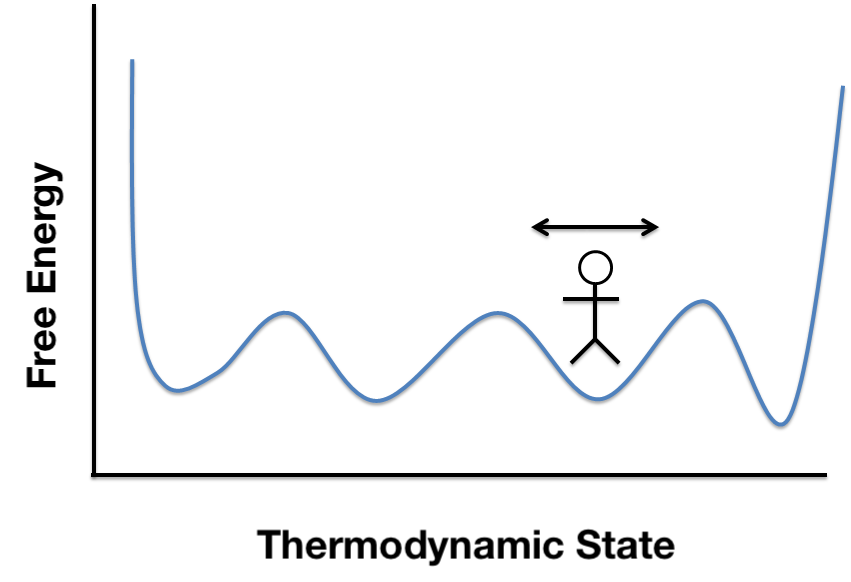
\includegraphics[width=\textwidth]{Figures/emptywell.png}
\caption{Beginning of Simulation}
 \label{fig:emptywell}
\end{subfigure}%
~
\begin{subfigure}[b]{0.33\textwidth}
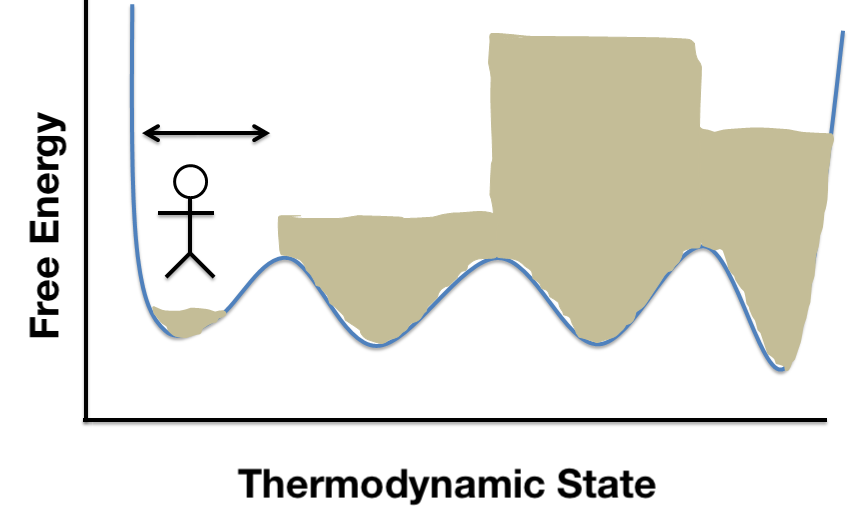
\includegraphics[width=\textwidth]{Figures/halfwell.png}
\caption{During Simulation}
\label{fig:halfwell}
\end{subfigure}
~
\begin{subfigure}[b]{0.33\textwidth}
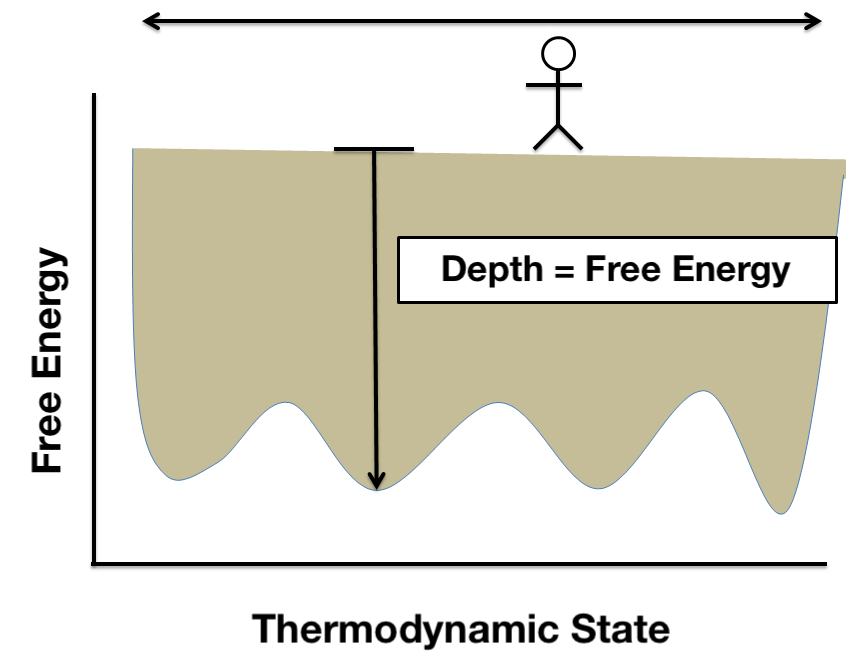
\includegraphics[width=\textwidth]{Figures/fullwell.png}
\caption{End of Simulation}
\label{fig:fullwell}
\end{subfigure}
\caption{The expanded ensemble hole analogy. (\ref{fig:emptywell}) At the beginning the biasing weights as a function of thermodynamic state are unknown. (\ref{fig:halfwell}) As the simulation proceeds, a random walker samples the states and deposits ``dirt'' (probability of visitation) in each location.  The short arrow over the random walker signifies uneven sampling of the states as the the biases are built adaptively.  (\ref{fig:fullwell}) At the end of the simulation, the weights, given by the height of ``dirt'', in each well are equal to the free energy.  The random walker now samples all states equally, as illustrated by the long bar over the walker which now extends over all of state space.} \label{fig:EXEanalogy}
\end{figure*}

\begin{comment}
We consider a set of $K$ thermodynamic states defined
by their thermodynamic parameter vectors, $\lambda_k \equiv \{\beta_k,
\mathcal{H}_k, p_k, \vec{\mu}_k, \ldots\}$, with $k = 1,\ldots,K$, where $H_k$
denotes any modifications of the Hamiltonian $H$ as a function of $k$,
including biasing potentials.  Each new choice of $k$ gives rise to a
\hyperlink{ref:reduced} {reduced} potential $u_k$, unnormalized and normalized probability
distributions $q_k(\vx)$ and $\nu(\vx,k)$, and a partition function $Z_k$.
To ensure that any configuration $x$ has finite, nonzero density in
all $K$ thermodynamic states, we additionally require that the same
thermodynamic parameters be specified for all thermodynamic states,
though their values may of course differ.
\end{comment}

Transitions between the subensembles labeled by indices $k$ or equivalently discrete values of a vector $\mathbf{\lambda}$ can most simply be performed by \hyperlink{ref:MetropolisMonteCarlo} {Monte Carlo}~\footnote{Molecular dynamics is also possible, but we will restrict our discussion of transitions
between states to Monte Carlo for now, as dynamics in a continuous $\mathbf{\lambda}$ has a number of additional subtleties and is much less common.}.  We can use any proposal/acceptance scheme that ensures this conditional distribution is sampled in the long run for any fixed $\vx$. At each step, we can choose to sample in either $k$ or $\vx$ according to some fixed probability $p$.  We can also alternate $N_k$ and $N_x$ steps of $k$ and $\vx$ sampling, respectively.  Although this Gibbs sampling algorithm does not satisfy detailed balance, it does satisfy the weaker condition of \emph{balance}~\cite{deem:jcp:1999:balance} which is sufficient to preserve sampling from the joint stationary probability distribution $\nu(\vx,k)$.  When proposal probabilities are based on past history, however, the algorithm will not preserve the equilibrium distribution~\cite{reinhardt:cpl:2000:step-size-adjustment}, though in some cases the deviations caused by the history dependence can be mitigated with proper choices of parameters (as shown in the parallel case of metadynamics)~\cite{bussi.equilibriummetadynamics}.

One possibility is to make steps to neighboring states, much like in replica exchange; if the states have a natural ordering, this is perfectly reasonable. However, they may not be a natural ordering, for example when there are multiple neighboring states in dimension higher than one, or if temperature and external biases are combined.

If we think of sampling this joint space in configuration and state in the context of Gibbs sampling, an \hyperlink{ref:ExpEns} {expanded ensemble} simulation can proceed by alternating between sampling from the two conditional distributions,
\begin{eqnarray}
\nu(\vx | k) &=& \frac{q_k(\vx)}{\int_\Gamma  \, q_k(\vx) \, d\vx}  = \frac{e^{-u_k(\vx)}}{\int_\Gamma  \, e^{-u_k(\vx)} \, d\vx }  \\
\nu(k | \vx) &=& \frac{e^{g_k}q_k(\vx)}{\sum\limits_{k'=1}^K e^{g_{k'}}q_{k'}(\vx)} = \frac{e^{g_k - u_k(\vx)}}{\sum\limits_{k'=1}^K e^{g_{k'} - u_{k'}(\vx)}} .\label{equation:expanded-ensemble-gibbs-update}
\end{eqnarray}

Sampling from the conditional probability distribution
$\nu(\vx | k)$ is just standard molecular sampling that generates correlated samples. Fortunately, the sampling in $\nu(k | \vx)$ is often much simpler.   If we have
discrete states which can be enumerated, we can simply calculate
$u_k(\vx)$ for each state and select randomly with $\nu(k|\vx)$.  The
probabilities only depend on the \hyperlink{ref:reduced} {reduced} energy differences $\Delta
u_{ik}(\vx) = u_i(\vx) - u_k(\vx)$, which is often much cheaper to calculate
than $u_k(\vx)$ is. Sampling in this way is often significantly easier with expanded ensemble than with replica exchange. In replica exchange, often each state is only stored on a single replica, and communicating the energy between states is complicated. With expanded ensemble, all of the states are being kept track of by the simulation, so calculating the conditional probabilities of the other states is relatively straightforward.

\subsubsection{\label{sec:singlestate} Methods updating biases one state at a time}
Given ways to sample between the states, we now need methods that adaptively change the biases $g_k$ until sampling of the different states reaches the desired ratio. The simplest way to update biases is to do it one state at a time, where the state that is currently visited is the one that is changed. Other schemes will introduce updating the bias of several schemes at a time.

\textbf{Wang-Landau updating}:
%\textbf{Describe WL, cite paper:\cite{wang-landau:prl:2001:wang-landau}, delta incrementation, cite the 1/t articles for long time scale behavior papers: \cite{Belardinelli2008, Belardinelli2007}.  Paper for Expanded Ensemble with WL walks in Alchemical States: \cite{Aberg_Lyubartsev}.}
If subensemble weighting factors $g_k$ are equal to \hyperlink{ref:reduced} {reduced} free energies then one will eventually obtain even sampling of all the states
\cite{lyubartsev:jcp:1992:expanded-ensembles}.  One procedure for the
iterative calculation of these biasing weights is the Wang-Landau
algorithm \cite{wang-landau:prl:2001:wang-landau}. This was originally proposed to calculate biasing weights where the different values of the total energy are the different thermodynamic states, in which case these biasing weights $g_k$ are equal to the density of states $\Omega(U)$ (see Section~\ref{sec:abp_energy}).  However, it has also been used as a general approach to calculate biasing weights associated with other ensembles.

The approach is described as follows: a histogram of visitations to each thermodynamic state
during the \hyperlink{ref:ExpEns} {expanded ensemble} simulation, $h(i)$ is maintained
throuhout the simulation.  When a state is visited, the corresponding
histogram entry is updated by 1.  In addition the weighting factors $g_i$ of that state is updated by $-\delta$, where $\delta$ is reduced by a monotonically decreasing function as the simulation proceeds.  The
weight of the reference state is zeroed after each step.

\begin{eqnarray}
h_{\mathrm{new}}(i) = h_{\mathrm{old}}(i) + 1 \\
g_{i,\mathrm{new}} = g_{i,\mathrm{old}} - \delta
\label{eq:wang-landau}
\end{eqnarray}

The Wang-Landau algorithm is self-correcting; if a state is visited more frequently than it would be under equal sampling of all of the states, its weight decreases accordingly, resulting in fewer visits to that state.  Eventually the weight falls back to the correct range.  The $\delta$ increment is decreased during the simulation when the histogram $h(i)$ reaches a specified flatness criteria, often set at 80\%~\cite{wang-landau:prl:2001:wang-landau}.  When a sufficiently flat histogram is achieved, $\delta$ is reduced by multiplying by a scaling factor $0<s<1$, typically $1/2$ as proposed in the original algorithm~\cite{wang-landau:prl:2001:wang-landau}.

\textbf{$1/t$ modifications to Wang-Landau}

The Wang-Landau updating scheme can lead to saturation in the error,
meaning that on average, simulations will get stuck at weights that do
not converge to the true answer~\cite{Belardinelli2008,
  Belardinelli2007}.  This saturation will occur at $s$, and taking $s$ close to one will delay this saturation at the
cost of slower convergence.

To avoid this saturation of error, Belardinelli and Pereyra proposed a
power law update to $\delta$, independent of histogram flatness at
long time scales. This update to Wang-Landau, called the $1/t$ method
scales $\delta$ as $1/t$, where $t$ is the \hyperlink{ref:MetropolisMonteCarlo} {Monte Carlo} time, \textit{e.g.} the
number of attempted state transitions.  Belardinelli and Pereyra
suggest starting with a standard Wang-Landau algorithm, and then
switching to using weights of $1/t$ when $\delta \leq 1/t$~\cite{Belardinelli2008, Belardinelli2007}. This scaling has also been noted by statisticians~\cite{wl_convergence}).

% \subsection{\label{sec:multiplestatemethods}Multiple State \hyperlink{ref:Reweighting} {Reweighting} Methods}
\subsubsection{\label{sec:multiplestatemethods}Multiple State Reweighting Methods}

The Wang-Landau approach and its $1/t$ variant only update the free energy of one state at one time, i.e. when it is visited during the random walk in the \hyperlink{ref:ExpEns} {expanded ensemble}.  However, in theory, it should be possible to update the weights of multiple states at the same time, based on information obtained at any given state.

A number of closely related methods have been developed that update multiple states simultaneously. The key to these approaches is recognizing that the same information needed to correctly calculate the probability of  transitions between states (i.e. the transition matrix) is the same information that is needed to calculate the free energy differences between the same states~\cite{escobedo_transition_2006,Wang:JoSP:2002} (see Section~\ref{sec:transtion_matrix}).

\textbf{Transition Matrix Approaches}
%JH \hyperlink{ref:MetropolisMonteCarlo} {Monte Carlo} Approaches}

The simplest way to use this concept is to directly compute the transition matrix and calculate free energies from this matrix~\cite{siderius_2013}. Assuming one uses \hyperlink{ref:MetropolisMonteCarlo} {Metropolis Monte Carlo}, we collect the transitions from each state $i$ to $j$ in a matrix $C$

It can be updated with any of:
\begin{enumerate}
\item Transitions actually performed (adding 1 if the transition occurs, 0 if it does not)\label{item:actual}
\item The probability of acceptance of a proposed move whether or not it was accepted.\label{item:proposal}
\item The probability of acceptance of any move transition that could have been proposed, independent of the algorithm actually used to perform the move. \label{item:transition}
\end{enumerate}

The free energy difference between any two states $i$ and $j$ can then be estimated as
\begin{equation}
f_{ij} = - \ln \langle C_{ij}/C_{ji} \rangle
\label{eq:transitionmc}
\end{equation}

\textbf{Asymptotically Optimal Weights}
We can also update all weights simultaneously by \hyperlink{ref:Reweighting} {reweighting} the
information gathered at the current state.   Several variants of this approach have been proposed. These include the accelerated weight histogram (AWH) method
\cite{Lidmar2012} and the independently developed self-adjusted mixture sampling (SAMS)~\cite{tan_optimally_2017}.

The basic idea of these variants is to use the Gibbs sampler to transition between states. After $N_x$ configurational updates with fixed state $i$, a new state $j$ is proposed by the Gibbs sampler probabilities $\alpha(j|\vx, i)$:
\begin{equation}\label{eq:gibbsproposal}
  \alpha(j|\vx, i) = \nu(i|\vx)
\end{equation}
where $\nu(i|\vx)$ is given in Equation~\ref{equation:expanded-ensemble-gibbs-update}.

In the self-adjusted mixture sampling variant, the weights are updated at each step. Using the transition rule defined in eq.~\ref{equation:expanded-ensemble-gibbs-update}, the rule for updating is:
\begin{eqnarray}
g_{i,new} = g_{i,old} - t^{-1}\nu(\vx|k)
\end{eqnarray}
where $t$ is a timescale that is ideally the number of uncorrelated steps in $(k,\vx)$ space that have been taken in the algorithm so far.\footnote{$t$ is not necessarily the number of timesteps taken so far in the simulation: if the correlation time in configuration space is slow, then updating the weights at every step, or updating them every step without a scaling factor to make their contribution smaller might lead to premature convergence of the biases on a subset of the conformational states.}

In the accelerated weight histogram approach, instead a histogram of the weights for each state is maintained during the simulation. The weight histogram is then updated using the computed $\nu(i|\vx)$ weights:
\begin{equation}
h_{\mathrm{new}}(i) = h_{\mathrm{old}}(i) + \nu(i|\vx)
\label{eq:awh-weight-histogram}
\end{equation}

Every $N_I$ iterations, the simulation weights are updated according to:
\begin{equation}
g_{i,\mathrm{new}} = g_{i,\mathrm{old}} - \ln{\frac{h_{\mathrm{new}}(i)K}{N}}
\label{eq:awh_free_energy_up}
\end{equation}
where $N$ is the total number of samples collected up to that point.

\begin{comment}

which states:
\begin{equation}
\xi^{(t-\frac{1}{2})} = \xi^{(t-1)} + t^{-1}\left\{w_i(X_t);\xi^{(t-1)})/\pi_i,...,w_m(X_t;\xi^{(t-1)})/\pi_m\right\}^T
\end{equation}
Translating from Tan's
terminology, $t$ is the current step of \hyperlink{ref:MetropolisMonteCarlo} {MC}/MD sampling, the $\xi^{(t-\frac{1}{2})}$ is the vector of $g_{i,new}$ and $\xi^{(t-1)}$ is the vector of $g_{i,old}$. Tan's $X_t$ is the same as $\vx$ in the current terminology, and and $\pi_i$ are the \hyperlink{ref:targetdist}{target probability distributions} of each state; if we assume we are looking for equal sampling of the states, they are all simply equal to 1; we will look at other variations later. $w_j(X;\xi)$ is the expectation of the \hyperlink{ref:MetropolisMonteCarlo} {Monte Carlo} transition probability to state $j$ states when the current configuration is $X$, and the current weights are $\xi$.

\end{comment}

\textbf{Multiple state reweighting as optimally reweighted Wang-Landau method}

This introduces a variant of a Wang-Landau-like algorithm with a basis in multistate \hyperlink{ref:Reweighting} {reweighting} techniques. We start with MBAR, the provably minimum variance \hyperlink{ref:FEestimator} {free energy estimator} given $N_{i}$ samples from each of $i=1 \ldots K$ states. \cite{shirts-chodera:jcp:2008:mbar}.  The estimator for the \hyperlink{ref:reduced} {reduced} free energy for each state $f_{i}$ up to an additive constant is given by the following self-consistent equation \cite{shirts-chodera:jcp:2008:mbar}:

\begin{eqnarray}
\exp(-f_i) = \sum_{n=1}^N \frac{\exp(-u_i(\vx_n))}{\sum_k N_k \exp(f_k-u_k(\vx_n))}
\label{eq:MBARwl}
\end{eqnarray}

Assuming that after $n$ steps of simulation, we have a decent estimate of the free energies $\hat{f}_{i}$ and that we wish to add one more sample without recalculating the free energies explicitly. We obtain:
\begin{eqnarray}
\hat{f}_{i}^{(N+1)} &\approx& \hat{f}_{i}^{(N)}- \frac{\exp(\hat{f}_{i}^{(N)}-u_i(\vx_{N+1}))}{\sum_k N_k \exp(\hat{f}_{k}^{(N)}-u_k(\vx_{N+1}))}
\label{eq:WWL}
\end{eqnarray}

Interestingly, we note that this is equivalent to self-adjusted mixture sampling, as well as nearly the same as AWH for updating the weights of each state. Specifically, because at step $N$, the weight sum is reset to $N/K$, and the right term in Equation~\ref{eq:WWL} is the weight update term of AWH. Therefore, AWH is similar to the
optimal approach (SAMS / weighted Wang-Landau) except that the free energies are only updated every
$N_I$ steps, and $N_k = N/K$ for all states is assumed, rather than using the current exact $N$.

\subsubsection{Initializing Biasing Weight}

One common problem with all of these near optimal methods is that they are only optimal in the asymptotic limit, when a large number of uncorrelated samples have been collected.  If only a small number of samples have been collected, they may not converge quickly, and indeed may tend to keep samples in the same thermodynamic state for quite a while.

It is still not clear what the best approach is to initialize the biasing weights until the number of samples reach the asymptotic limit.  The current general approach is to run the original Wang-Landau approach with a large initial increment size without reducing the weights until some predetermined point. This predetermined point varies between approaches and implementations.  One is to stay in this initial phase until the histograms are roughly equal and then switching to a variant of the asymptotically optimal method~\cite{tan_optimally_2017}. However, it is not really known if this is optimal, and there are still choices to make, such as the initial bias added to each step.

\subsubsection{Public implementation of expanded ensemble methods}

Of these different variants of expanded ensemble, the SAMS version is implemented in OpenMM~\cite{10.1371/journal.pcbi.1005659}, and GROMACS~\cite{lindahl_2021} implements both the AWH and the weighted Wang-Landau approach.

\section{Adaptive seeding methods}
\label{sec:seeding}
\subsection{Adaptive sampling}
\hyperlink{ref:Adaptive} {Adaptive} \hyperlink{ref:Seeding} {seeding} seeks to sample the configurational space by focusing simulation efforts in regions that will lead to a more accurate description of the ensemble. It generally takes advantage of analysis methods such as Markov State Modeling to then stitch together trajectories and build a coherent model of, not only the equilibrium population of metastable states, but also the rates of conversion between these states.

\hyperlink{ref:Adaptive} {Adaptive} \hyperlink{ref:Seeding} {seeding} methodologies were mostly developed with the problem of protein folding in mind, a process that is characterized by rare transitions along a pathway to a single folded state. In such an application, observing a rare event for which a free energy barrier needs to be crossed only depends on the aggregated simulation time, not the length of the simulation so far, because the probability of overcoming a free energy barrier depends on the total number of attempts made at crossing it \cite{PhysRevLett.86.4983,doi:10.1021/acs.jctc.8b00500}. Adaptive \hyperlink{ref:Seeding} {seeding} thus seeks to seed simulations from regions of space that are likely to lead to free energy barrier crossing in order to sample the entire configurational space, using the information acquired through the sampling so far. In other words, sampling over and over regions of space that have already been explored does not add valuable information, whereas crossing into regions of space not previously sampled adds valuable information to reconstruct probability distributions.

MSM building involves discretizing the configurational space into states (usually called microstates in the MSM literature, at odds with \hyperlink{Microstate} {the definition} used in this review) and estimating their probability distribution as well as the probability of transitions between these states for a given time lag $\tau$. Discretization of the space can in principle be done based on geometric criteria. However, since the focus of MSM building has been to extract kinetic properties, discretization has often been performed based on kinetic proximity, using time-lagged independent component analysis (TICA). The transition probabilities are gathered in a transition matrix $T_{ij}$ which records the probabilities of transitions from state $i$ to $j$ given a time lag $\tau$. Estimating the probability density directly from counting the number of configurations falling in a state would be incorrect for a strategically seeded ensemble. However, the fact that the transition probabilities are taken into account enables to reconstruct the probability density, see Section~\ref{sec:fe_estimators}. These microstates are generally then clustered into macrostates using a distance metric.


Different adaptive \hyperlink{ref:Seeding} {seeding} strategies have been put forward. They all follow the same basic algorithm: a single or a set of relatively short MD simulations are launched. Configurations from these simulations are grouped into ``states". New simulations are then started from selected states. The different strategies then differ according to the principle they follow to select which states to seed new simulations from.
Arguably the first proposed strategy relied on selecting randomly a fixed number of structures from each macrostate~\cite{doi:10.1063/1.2740261,Huang19765,doi:10.1021/ct900620b}. This method was coined adaptive \hyperlink{ref:Seeding} {seeding}. In contrast, all the more refined methods derived therefrom and listed below are referred to as adaptive sampling. Another natural proposal has been to seed simulation from states that contribute the most to the statistical uncertainty of MSMs built after each iteration \cite{doi:10.1021/ct500827g}. Several variants have proposed to seed from low-population microstates, and have been called ``counts" methods. This strategy is well-suited to enhance the exploration of space, but not necessarily to accurately estimate the probability distribution of low free energy states \cite{doi:10.1021/ct2004484,doi:10.1021/ct400919u,lecina_adaptive_2017,shamsi_enhanced_2017,6114444}. \hyperlink{ref:Seeding} {Seeding} from low-population macrostates has also been suggested. This is better suited to converge the free energy calculation but will not lead to as an extensive space exploration \cite{doi:10.1021/acs.jctc.6b00762,doi:10.1063/1.5053582}. There are also methods that do not rely on MSM analysis. iMapD relies on clustering in a low-dimensional manifold inferred by \hyperlink{ref:DimRed} {dimensionality reduction} and selecting states to seed from the boundaries of a diffusion map in diffusion coordinates \cite{ChiavazzoE5494}.\footnote{iMapD does not enable the direct estimation of probability distributions.} Following a similar approach, it has been suggested to pick configurations to reseed from using multidimensional scaling-like embedding (sketch-map) \cite{doi:10.1021/acs.jctc.6b00503}. PIGS, for Progress Index Guided Sampling, uses an unsupervised heuristic to avoid re-sampling the same region of space by organizing simulation frames along a progress index that connects configuration to existing configuration by finding the one to which a chosen distance is minimal. Weakly connected snapshots that have a large distance to other configurations are used to start \hyperlink{ref:Seeding} {Seeding} new trajectories \cite{BACCI2015889}. Methods introducing directionality into the sampling have also been suggested and are particulary interesting when the target state (or set of states) is known. Broadly speaking, those suggest \hyperlink{ref:Seeding} {seeding} from states that are close to the end state in terms of a target property:
    \begin{enumerate}
    \item AdaptiveBandit expands on the methods described above by proposing to formulate the \hyperlink{ref:Adaptive} {adaptive} sampling problem in terms of reinforcement learning. This offers the promise and the computational platform needed to increased performance and flexibility of the algorithm across different systems \cite{doi:10.1021/acs.jctc.0c00205}.
    \item Reinforcement Learning Based Adaptive Sampling (REAP) proposes to efficiently explore configuration space by using reinforcement learning to choose new states. It does so by learning the relative importance of candidate \hyperlink{ref:CV} {collective variable}s as it makes progress along the \hyperlink{ref:FES} {landscape}, in a framework that rewards actions that lead to further exploration of the \hyperlink{ref:FES} {landscape}. Here too, states to learn from are selected as the least sample microstates. In that sense, it is a derivative of the counts method \cite{doi:10.1021/acs.jpcb.8b06521}.
    \item The Fluctuation Amplification of Specific Traits (FAST) method proposes to choose new states based on an objective function that balances trade-offs between exploring novel regions of space (exploration) and focusing on regions that are important to lead to a converged estimate of the target properties (exploitation) \cite{doi:10.1021/acs.jctc.5b00737,doi:10.1021/acs.jctc.8b00500} The parameter that balances these two aspects needs to be tuned, a non-trivial aspect of using this method. This method has been recognized to be a specific case of a multi-armed bandit problem.
    \item Specifically for protein folding, or conformational changes in biological molecules, a common target property is inter-residue contacts, or its opposite, minimizing non-desirable contacts \cite{doi:10.1063/1.5053582}
    \item In the same vein, it has been suggested to use evolutionary information by deriving inter-residue contacts from a multiple-sequence alignment, in a method called evolutionary couplings-guided \hyperlink{ref:Adaptive} {adaptive} sampling \cite{shamsi_enhanced_2017}
    \end{enumerate}


Attempts at a quantitative comparison of several of these \hyperlink{ref:Adaptive} {adaptive} sampling methods have been published \cite{doi:10.1063/1.5053582,doi:10.1021/acs.jctc.8b00500}, but a systematic comparison is still missing. Preliminary work indicates that accelerating rare event is better achieved with macrostate count or directed methods, while exploring the space is most efficient using microstate count~\cite{doi:10.1063/1.5053582}. Methods explicitly taking into account the tradeoff between exploitation and exploration can be more versatile in their usage.

\subsection{Weighted ensemble simulations - splitting/replication strategies}

The weighted ensemble (WE) method, also referred to as a splitting/replication approach, is particularly well-suited to exhaustively find pathways between macrostates and evaluate kinetic properties \cite{HUBER199697}. The approach relies on running relatively short MD simulation and terminating simulations that are not making progress towards the target state while replicating simulations that are instead progressing towards the end state \cite{doi:10.1146/annurev-biophys-070816-033834}. By keeping track of the total number of trajectories, the approach is statistically rigorous. Clustering into pathway ensembles can provide a rigorous estimate of the relative importance of the different pathways.

Because of their \hyperlink{ref:OutOfEq} {non-equilibrium} nature, this variety of enhanced sampling methods is not particularly well-suited to calculate equilibrium population distributions. However, even if weighted ensemble simulations do not achieve steady state, frameworks have been proposed to recover equilibrium properties \cite{doi:10.1063/1.3456985,doi:10.1021/ct401065r,doi:10.1021/jacs.8b10735}.

We note that weighted ensemble methodologies, while falling under the umbrella of adaptive \hyperlink{ref:Seeding} {seeding} strategies, can be categorized under transition path-finding methods, along with the string method with swarms of trajectories~\cite{doi:10.1021/jp0777059}, milestoning~\cite{doi:10.1063/1.1738640}, transition interface sampling~\cite{doi:10.1063/1.1562614}, forward flux sampling~\cite{PhysRevLett.94.018104}, Adaptive Multilevel Splitting~\cite{cerou-guyader-lelievre-pommier-11,teo-mayne-schulten-lelievre-16} and supervised unbiased MD~\cite{doi:10.1021/acs.jcim.9b01094, doi:10.1021/acs.jcim.5b00702}. We choose here to not review these methods in detail given the focus of this review on estimating configurational averages (see instead reviews \cite{doi:10.1146/annurev.physchem.040808.090412, doi:10.1146/annurev.physchem.53.082301.113146, doi:10.1063/1.5127780}).
The Weighted Ensemble method is implemented in the WESTPA software. Given the versatility of the framework, strategies and schedules can be easily explored \cite{Bogetti2019Suite}.

\section{Adiabatic methods}
\label{sec:adiab}
Adiabatic methods for free energy calculations generally refer to techniques where some timescale separation between the dynamics along the \hyperlink{ref:CV} {collective variable} (or the external parameter in an alchemical setting) is assumed, or artificially enforced, in order to obtain an (almost) Markovian dynamics along the \hyperlink{ref:CV} {collective variable} (respectively the auxiliary variable). This was first introduced as the adiabatic free energy dynamics (AFED) method~\cite{doi:10.1063/1.1448491}.

For example, the temperature accelerated molecular dynamics~\cite{MV06} (TAMD) consists in adding an extended degree of freedom $\lambda$, with mass $m_\lambda$, and a harmonic coupling potential $k^\mathrm{ext} \left( \xi(\vx) - \lambda \right)$.
The extended \hyperlink{ref:Langevin} {Langevin dynamics} reads:
\begin{equation}
\left\{
\begin{array}{ll}
    d\vx &= M^{-1} \vp \,  dt \\
    d\vp &= \left(-\nabla_\vx U(\vx) + k^\mathrm{ext} ( \lambda -\xi(\vx)) - \gamma \vp \right) dt
    + \sqrt{ \frac{2 \gamma M}{\beta}} \; d\mathbf{W}_t \\
    d\lambda &= m_\lambda^{-1} p_\lambda \, dt\\
    d p_\lambda &= \left( k^\mathrm{ext} (\xi(\vx) - \lambda)  - \overline\gamma p_\lambda \right) dt
    + \sqrt{ \frac{2 \bar\gamma m_\lambda}{ \overline\beta}} dW_t
\end{array}
\right.
\end{equation}

Note that the Langevin equation on $\lambda$ is based on a separate temperature factor $\overline \beta$ and friction coefficient $\overline{\gamma}$.

The basis of the TAMD method is that in the regime
\begin{equation}
\overline{\gamma} \gg \gamma \text{ and }\beta \gg \frac{1}{k^\mathrm{ext}},
\end{equation}
(considering the case where $\xi$ is dimensionless) the dynamics on $\lambda$ becomes uncoupled from the dynamics of $\vx$ and converges to an effective dynamics of the form:
\begin{equation}\label{eq:eff_dyn_z_bar}
d\lambda = - \frac{1}{\overline{\gamma}} \nabla F (\lambda) \, dt + \sqrt{ \frac{2}{\overline{\beta} \, \overline{\gamma}}} \, dW_t,
\end{equation}
so that the probability distribution sampled by $\lambda$ is (in this limiting regime) proportional to $\exp(- \overline{\beta} A(\lambda))$. The artificial inverse temperature $\overline{\beta}$ is then chosen so that the effective dynamics~\eqref{eq:eff_dyn_z_bar} is less metastable.
The practical difficulty of such a method is to choose the numerical parameters $(\gamma,\overline{\gamma},k^\mathrm{ext},\overline{\beta})$ for the algorithm to be efficient while keeping the adiabatic separation between the extended coordinate and the physical system -- failure to do so introduces a bias in the simulation.
In the ``single sweep" method, TAMD is used to estimate local free energy gradients, followed by estimation of the free energy surface.\cite{Maragliano2008}

Driven-AFED (d-AFED)~\cite{doi:10.1021/jp805039u}, unified free energy dynamics (UFED)~\cite{doi:10.1063/1.4733389}, canonical adiabatic free energy sampling (CAFES)~\cite{doi:10.1021/jp013346k} and on-the-fly free energy parameterization (OTFP)~\cite{ABRAMS2012114} are all related to this scheme.

Note also that conventional (non well-tempered) metadynamics (see Section~\ref{sec:meta-classic}) implicitly makes such an adiabatic hypothesis to get an unbiased \hyperlink{ref:FEestimator} {free energy estimator}~\cite{laio-gervasio-08, jourdain-lelievre-zitt-21}.


\section{Hybrid methods}
\label{sec:hybrids}

Enhanced sampling methods leveraging different principles can be combined together leading to hybrid schemes.
For example, a common theme is to combine an enhanced sampling method that focuses on biasing specific degrees of freedom or CVs (e.g., ABP methods such as metadynamics) with a enhanced sampling method that more generally enhances the sampling of a large number of, or even all, degrees of freedom (e.g., replica exchange methods). In this way, one can better sample slow orthogonal degrees of freedom that are missing in the biased CV set.
Another common combination is to complement a sampling method with an external \hyperlink{ref:FEestimator} {free energy estimator}. Several variants of these combinations have been presented in Sections~\ref{sec:eABF}, \ref{sec:adiab}, and~\ref{sec:metad_obtaining_fes}.
In addition, path finding methods like the string-of-swarms method can be combined with, e.g. umbrella sampling along the discretized minimum path obtained by the path finding method~\cite{doi:10.1021/jp0777059}. This is followed by free energy estimation along path coordinates.

There are so many possible combinations of enhanced sampling methods that it is difficult to offer a comprehensive discussion of all hybrid methods. Thus, we limit ourselves to discuss a few notable combinations below.


\subsection{Combination of replica exchange and external biasing potential methods}

Many hybrid enhanced sampling methods are a combination of Hamiltonian replica exchange and methods incorporating an external bias potential, which can be static or adaptively updated (e.g., umbrella sampling and metadynamics). Each replica $i$ includes its own bias potential $U^{\mathrm{bias}}_{i}(\vz)$, which depends on a \hyperlink{ref:CV} {collective variable} set $\vz_{i} = \xi_{i}(\vx)$ that can differ between replicas. Within each replica, the bias potential is kept static or evolved according to the adaptive biasing potential method. When calculating the acceptance probability $P_\mathrm{accept}(\vx_i, i, \vx_j, j)$ for an exchange of configurations $\vx_{i}$ and $\vx_{j}$ between two replicas $i$ and $j$ given in in Equation~\ref{eq:re_exchange_prob}, we need to take the bias potentials into account. We limit ourselves to the, still rather general, case that all replicas have same potential energy function $U(\vx)$ but can have different temperatures.

We start by rewriting the exchange acceptance probability given in Equation~\ref{eq:re_exchange_prob}
as\footnote{Note that we use here full quantities rather than \hyperlink{ref:reduced} {reduced} quantities as in Section~\ref{sec:generalized-ensemble}. However, the discussion is also valid for canonical and isothermal-isobaric ensembles.}
\begin{align}
\label{eq:replexc_acceptance probability}
P_\mathrm{accept}(\vx_i, i, \vx_j, j) &=
\min\left\{1,\frac{\exp(-[\beta_{i}U(\vx_j)+\beta_{j}U(\vx_i)])}{\exp(-[\beta_{i}U(\vx_i)+\beta_{j}U(\vx_j)])}\right\}
\nonumber \\
&=
\min\left\{1,\exp\left(\left(\beta_{i} - \beta_{j}\right)
\left[U(\vx_{i}) - U(\vx_{j})\right]\right)\right\}
\nonumber \\
&=
\min\left\{1,\exp \Delta_{i,j}\right\},
\end{align}
where we have defined $\Delta_{i,j}=\left(\beta_{i} - \beta_{j}\right)
\left[U(\vx_{i}) - U(\vx_{j})\right]
$ as the exponential term for conventional replica-exchange.

Incorporating the effect of the bias potentials, the exchange acceptance probability is calculated using the exponential term
\begin{align}
\Delta_{i,j} = &
\left(\beta_{i} - \beta_{j}\right)
\left[U(\vx_{i}) - U(\vx_{j})\right]
\nonumber \\ & +
\beta_{i} \left[
U^{\mathrm{bias}}_{i}(\xi_{i}(\vx_{i})) - U^{\mathrm{bias}}_{i}(\xi_{i}(\vx_{j}))
\right]
\nonumber \\ & +
\beta_{j} \left[
U^{\mathrm{bias}}_{j}(\xi_{j}(\vx_{j})) - U^{\mathrm{bias}}_{j}(\xi_{j}(\vx_{i}))
\right],
\end{align}
where the two last terms originate from the effect of the bias potentials acting on the two replicas~\cite{Bussi-JACS-2006}. In the following we discuss a few specific cases.

\subsubsection{Replica Exchange Umbrella Sampling}
\label{sec:repex_umbrsampl}
In replica exchange umbrella sampling~\cite{Sugita2000_REUS}, all the replicas are simulated at the same temperature but differ in the fact that the different replicas have their umbrella potential centered at different locations. Thus, by allowing exchanges between neighboring umbrella windows, the convergence is improved. The exchange also helps with sampling orthogonal slow degrees of freedom not included in the \hyperlink{ref:CV} {CV} set. The exchange probability is obtained using
\begin{align}
\Delta_{i,j} = &
\beta \left[
U^{\mathrm{bias}}_{i}(\xi(\vx_{i})) - U^{\mathrm{bias}}_{i}(\xi(\vx_{j})) +
U^{\mathrm{bias}}_{j}(\xi(\vx_{j})) - U^{\mathrm{bias}}_{j}(\xi(\vx_{i}))
\right],
\end{align}
where the bias potential correspond to different umbrella sampling windows (generally neighbouring windows).

\subsubsection{Parallel-Tempering Metadynamics}
Metadynamics can be combined with parallel-tempering to help with sampling missing slow orthogonal degrees of freedom not included in the biased \hyperlink{ref:CV} {CV} set~\cite{Bussi-JACS-2006}. The exchange probability is obtained using
\begin{align}
\label{eq:exchange_prob_ptmetad}
\Delta_{i,j} = &
\left(\beta_{i} - \beta_{j}\right)
\left[U(\vx_{i}) - U(\vx_{j})\right]
\nonumber \\ & +
\beta_{i} \left[
U^{\mathrm{bias}}_{i}(\xi(\vx_{i})) - U^{\mathrm{bias}}_{i}(\xi(\vx_{j}))
\right]
\nonumber \\ & +
\beta_{j} \left[
U^{\mathrm{bias}}_{j}(\xi(\vx_{j})) - U^{\mathrm{bias}}_{j}(\xi(\vx_{i}))
\right].
\end{align}
The same idea can also be used for other ABP methods (e.g., variationally enhanced sampling). In a similar way, metadynamics (and other ABP methods) can be combined with other replica exchange methods such as replica exchange solute tempering~\cite{REST2_Wang_2011,HREX_Bussi_2013}, that have a better scaling in term number of replicas needed. Then the first term in Equation~\ref{eq:exchange_prob_ptmetad} would be adjusted while the last two terms would remain the same.

\subsubsection{Bias-Exchange Metadynamics}
\label{sec:be-metad}
Bias-exchange metadynamics~\cite{Piana2007_bemeta} allows for biasing a large set of \hyperlink{ref:CV} {CV}s simultaneously by considering multiple replicas running at the same simulation temperature, but each biasing a different set of \hyperlink{ref:CV} {CV}s using metadynamics. Generally, one considers one \hyperlink{ref:CV} {CV} per replica so the outcome are several one-dimensional free energy \hyperlink{ref:FES} {profile}s. By allowing for exchange of configurations between replicas, we can avoid the problem of missing slow orthogonal \hyperlink{ref:CV} {CV}s in each replica.
The exchange probability is obtained using
\begin{align}
\Delta_{i,j} = &
\beta \left[
U^{\mathrm{bias}}_{i}(\xi_{i}(\vx_{i})) - U^{\mathrm{bias}}_{i}(\xi_{i}(\vx_{j})) +
U^{\mathrm{bias}}_{j}(\xi_{i}(\vx_{j})) - U^{\mathrm{bias}}_{j}(\xi_{i}(\vx_{i}))
\right].
\end{align}
Traditionally, bias-exchange is used with conventional (non-well-tempered) metadynamics but it can also be used with well-tempered metadynamics. We can even imagine using bias-exchange with other ABP methods such as variationally enhanced sampling.
%

\subsubsection{Parallel-Tempering in the Well-Tempered Ensemble}
\label{sec:pt-wte}
Combining parallel-tempering with the well-tempered ensemble~\cite{Bonomi-PRL-2010} (i.e., well-tempered metadynamics biasing the potential energy) allows to greatly reduce the number of replicas required for parallel-tempering simulations of solvated systems~\cite{Deighan2012_ptwte_efficient}. This comes from two effects. First, within each replica potential, energy fluctuations are enhanced by a factor of $\gamma$ while averages stay more or less the same, leading to a better potential energy overlap between replicas. Second, the $\Delta_{ij}$ factor used to calculate the exchange acceptance probability in Equation~\ref{eq:replexc_acceptance probability} is given as
\begin{align}
\Delta_{i,j} = &
\gamma^{-1}
\left(\beta_{i} - \beta_{j}\right)
\left[U(\vx_{i}) - U(\vx_{j})\right]
\end{align}
and thus reduced by a factor of $\gamma$ as compered to conventional replica exchange (Equation~\ref{eq:replexc_acceptance probability}),  which leads to higher exchange probability (if $\Delta_{i,j}<0$, otherwise if $\Delta_{i,j}>0$ the exchange acceptance probability is unity). Due to these two effect, one can use a larger temperature difference between replicas and thus require fewer replicas overall. Parallel-tempering in the well-tempered ensemble can also be combined with metadynamics where other \hyperlink{ref:CV} {CV}s are biased separately.

\subsubsection{Replica Exchange with collective variable tempering}
%JH \hyperlink{ref:CV} {collective variable} Tempering}

The idea behind replica exchange with \hyperlink{ref:CV} {collective variable} tempering~\cite{Gil-Ley_JCTC-2015} is to reduce the number of replicas needed for replica-exchange simulations by focusing only on selected degrees of freedom. One considers $M$ replicas with the same temperature and within each replica, one performs concurrent well-tempered metadynamics simulations where one considers the same \hyperlink{ref:CV} {CV} set within replica and biases each \hyperlink{ref:CV} {CV} by a separate one-dimensional metadynamics potential. One can then bias a large number of degrees of freedom (e.g., all dihedral angles). The replicas are arranged in a ladder of increasing bias factor values where the lowest replica corresponds to the canonical ensemble ($\gamma=1$). Thus, by going up the replica ladder, the fluctuations of the biased degrees of freedom are enhanced. Though one considers a large number of degrees of freedom, this is considerably smaller than the total number of the system's degrees of freedom. Therefore, the number of replicas needed is considerably less than parallel-tempering, where fluctuations of all degrees of freedom are enhanced by heating the system.

\subsection{Combination of metadynamics and other enhanced sampling methods}

Apart from the replica exchange-based hybrid methods discussed in the previous section, there are various other hybrid methods where metadynamics has been combined with other types of enhanced sampling methods. Furthermore, some of the variants of metadynamics listed in Section~\ref{sec:metad_variants} could be considered as hybrid methods, and vice versa, as the distinction between a variant and a hybrid method is not always so clear.

Metadynamics has been combined with methods that enhance the potential energy sampling (see Section~\ref{sec:abp_energy}) such as the multicanonical ensemble~\cite{Yonezawa_MulticanonicalMetaD_2011} and integrated tempering sampling~\cite{Yang_MetaD-ITS_1_2016,Yang_MetaD-ITS_2_2018}. Here the idea is similar as when metadynamics is combined with parallel tempering, this should help with sampling missing slow orthogonal degrees of freedom. In a similar spirit, variationally enhanced sampling has been combined with sampling in the multithermal-multibaric ensemble~\cite{Piaggi_MultiVES_2019,Piaggi_MultiVES+CV_2019}.

In driven metadynamics~\cite{Moradi_DrivenMetaD_JPCL2013}, metadynamics is combined with steered MD.
In orthogonal space random sampling (OSRW)~\cite{Zheng_OSRW-1_PNAS2008,Zheng_OSRW-2_JCP2009,Min_OSRW-3_JCTC2010}, metadynamics is combined with a procedure based on thermodynamic integration to facilitate sampling of orthogonal degrees of freedom. Metadynamics has been combined with umbrella sampling in various ways as we discuss in the following.

In Refs~\cite{Badin_MetaD-US-1_JCP2006,Autieri_MetaD-US-2_JCP2010}, metadynamics is used to generate a bias potential that leads to effective sampling and diffusion in the CV space. The bias potential is then used as a static bias potential in another simulations where the FES is calculated using umbrella sampling corrections (i.e., reweighting with a static bias potential).

In Ref~\cite{Zhang_MetaD-US-3_JCTC2013}, metadynamics is used to identify a pathway and then the free energy profile along the pathway is calculated using multiple window (localized) umbrella sampling.

In Refs~\cite{Johnston_MetaD-US-4_PLos2012,Awasthi_MetaD-US-5_JCC2016}, multiple windows (localized) umbrella sampling is used to bias some chosen CV while within each umbrella window, metadynamics is used to bias another set of CVs. The main idea behind this strategy is that umbrella sampling is more suited than metadynamics to bias CV whose free energy profile is broad. Furthermore, the metadynamics bias potential within each umbrella window helps to sample degrees of freedom that are orthogonal to the CV biased in the umbrella sampling simulations and thus improve the convergence. This combined umbrella sampling and metadynamics strategy has been extended to incorporate temperature accelerated MD~\cite{Awasthi_TASS_JCP2017,Pal_TASS-2_JCC2021} or replica exchange with solute tempering (REST2)~\cite{Kapakayala_WS-MetaD+REST2_JCC2021} to further improve the sampling of orthogonal degrees of freedom.


\subsection{Combination of metadynamics and structural ensemble determination methods}

Structural ensemble determination methods~\cite{Bonomi_StructEnsembleDeterm_Review_COSB2017,Cesari_MaximumEntropyPrinciple_Review_Comp2018,Bottaro_Science2018}, for example based on maximum entropy principle~\cite{Pitera_MaxEnt_JCTC2012,Roux_MaxEnt_JCP2013}, are used to integrate experimental observations into molecular simulations and yield structural ensembles that are compatible with experiments. While such structural ensemble determination methods are not strictly enhanced sampling methods, they are somewhat related as they generally introduce external restrains in the form of bias potentials that can be fixed or adaptively updated. To accelerate the configurational sampling, structural ensemble determination methods are often combined with enhanced sampling methods such as metadynamics.


In Ref~\cite{Bonomi_MetadynamicMetainference_SciRep2016}, parallel-bias metadynamics is combined with metainference~\cite{Bonomi_Metainference_SciAdv2016} that is a structural ensemble determination methods that incorporates experimental errors via a Bayesian inference framework. In Ref~\cite{Amirkulova_PTWTE-EDS_JPCB2020}, parallel-tempering in the well-tempered ensemble (Section~\ref{sec:pt-wte}) is combined with experiment directed simulations~\cite{White_EDS_JCTC2014}.
An older work along this line is replica-average metadynamics~\cite{Camilloni_RAM_2013,Camilloni_RAM-2_JACS20214}, where metadynamics or bias-exchange metadynamics is combined with replica-averaging.

Related to the idea of structural ensemble determination methods are experiment directed metadynamics~\cite{White_EDM_2015}, ensemble-biased metadynamics~\cite{Marinelli_EnsembleBiased_2015}, and target metadynamics~\cite{GilLey_TargetMetaD_2016}. In these variants of metadynamics, the bias updating procedure is modified such that the biased CV distribution that the simulation converges to is some predefined \hyperlink{ref:targetdist}{target probability distribution}. Thus, by taking this \hyperlink{ref:targetdist}{target distribution} from experimental measurements, it is possible to obtain a structural ensemble that is compatible with the experimental results. In a similar spirit, the \hyperlink{ref:targetdist}{target distribution} in variationally enhanced sampling~\cite{Valsson_VES_PRL_2014,Valsson2020Handbook_VES} (Section~\ref{sec:ves}) can be taken from experimental measurements.

\subsection{Combinations of ABF and other enhanced sampling methods}
\label{sec:abf_hybrids}

The ABF algorithm is applied within a defined region of collective variable space, where its application leads to improved sampling and yields an estimate of the free energy gradient. A localization approach (\ref{sec:localization}) can be used: ABF can be applied independently on several smaller, non-overlapping regions of the collective variable\cite{Chipot2005} or several variables\cite{Henin2010a}. This reduces the time needed for diffusive sampling of a large volume of CV space. Thanks to the local character of this gradient, the estimated gradient in all regions can be merged by simple concatenation, and then integrated in one piece~\cite{Henin2021integration}. Unlike energy-based methods like Umbrella Sampling, no particular precaution is necessary to match the data from different strata (windows).

Metadynamics has been combined with extended-system ABF~\cite{Fu_MetaD-eABF_JPCL2018,Fu_MetaD-eABF_JCIM2020} to improve the exploration properties of ABF.
For a review of these hybrid eABF methods, see~\cite{Fu2019}.
This combination has been further extended by incorporating Gaussian-accelerated MD~\cite{Chen_GAMD-MetaD-eABF_JCTC2021} to help sample orthogonal degrees of freedom not included in the biased CV set.

Orthogonal Space Tempering (OST) is a variant of OSRW based on an extended-system ABF method, using a finite sampling temperature in the orthogonal space.\cite{Zheng2012}
In this method, the ABF-like sampling of an alchemical parameter $\lambda$ is completed by enhanced sampling of the force along $\lambda$, which correlates with slow orthogonal degrees of freedom, thereby accelerating orthogonal relaxation.

\section{Software Implementations}
The codes to run the various simulations outlined in the previous sections range from in-house scripts, to methods implemented natively in the largely used MD simulation packages GROMACS, AMBER,  NAMD or CP2K, and via the open-access libraries or plugins Colvars~\cite{Fiorin2013}, PLUMED~\cite{Bonomi-CPC-2009,Tribello2014,plumed-nest}, PMFlib~\cite{kulhanek2011pmflib}, and SSAGES~\cite{Sidky2018}. The most popular software options for each method have been mentioned in the dedicated sections and are summarized in Tables~\ref{Table:Codes} and~\ref{Table:Libraries}.

Several free and open source codes are gathered under a GitHub topic: \url{https://github.com/topics/enhanced-sampling}

\begin{table*}[!ht]
\caption {Built-in capabilities of widely used molecular dynamics simulations codes. Methods not discussed in the text may be included, see user guides for more discussion.}
\label{Table:Codes}
\begin{tabularx}{0.95\textwidth}{
  || >{\raggedright\arraybackslash} l
  || >{\raggedright\arraybackslash}X
  | >{\raggedright\arraybackslash}l ||}
 \hline
  MD engine  & Main features                                 & Reference \\
\hline
\hline
CHARMM & Adaptively Biased Path Optimization (ABPO), Adaptive Umbrella Sampling, Constraints, Distributed CSA (Conformational Space Annealing), Dynamic Importance Sampling (DIMS), Enveloping Distribution Sampling Method, Replica Exchange, Free Energy Perturbation, Self-Guided Langevin Dynamics, String method, Targeted Molecular Dynamics, Transition Path Sampling & \cite{Brooks2009} \\
\hline
NAMD &  Simulated annealing, steered MD, (unconstrained variant of) targeted MD, accelerated and Gaussian-accelerated MD, custom algorithms via Tcl scripting, grid forces.        & \cite{Phillips2020} \\
\hline
GROMACS & Restraints (various potentials including harmonic potentials for umbrella sampling), simulated annealing, replica exchange, \hyperlink{ref:ExpEns} {expanded ensemble} (both as AWH and a separate implementation), \hyperlink{ref:OutOfEq} {non-equilibrium} pulling (steered MD), applying forces from three-dimensional densities.   &  \cite{lindahl_2021}\\
\hline
OpenMM & Simulated annealing, applying external forces, versatile python framework to implement any scheme, \hyperlink{ref:ExpEns}{expanded ensemble} (as self-adjusted mixture sampling). & \cite{10.1371/journal.pcbi.1005659}\\
\hline
AMBER  &  Replica exchange, targeted MD, steered MD, accelerated and Gaussian-accelerated MD, Self-Guided Langevin dynamics, applying external forces, umbrella sampling, string-of-swarms. & \cite{Case_2021} \\
\hline
CP2K & Constraints, Harmonic restraints, targeted MD, steered MD, metadynamics. & \cite{CP2K_2020} \\
\hline
DESMOND & Umbrella sampling, Metadynamics & \cite{Desmond2006} \\
\hline
LAMMPS  & Harmonic restraints, applying external forces, replica exchange, parallel replica dynamics, temperature accelerated dynamics, original hyperdynamics, local hyperdynamics. &  \cite{LAMMPS_2022}\\
\hline
HOOMD-blue &  Restraints, applying external forces, versatile python framework to implement any scheme. & \cite{HOOMD-blue_2020} \\
\hline
Tinker-HP & Steered MD, Gaussian-accelerated MD, umbrella sampling & \cite{Celerse2019,Celerse2021} \\
\hline
GROMOS & Replica Exchange, umbrella sampling, thermodynamic integration, enveloping distribution sampling.  & \cite{Gromos_2012} \\
\hline
\end{tabularx}
\end{table*}

\begin{table*}[!ht]
\caption {Libraries and Modules for enhanced sampling}
\label{Table:Libraries}
\begin{tabularx}{0.95\textwidth}{
  || >{\raggedright\arraybackslash}l
  || >{\raggedright\arraybackslash}X
  | >{\raggedright\arraybackslash}l ||}
\hline
  Library name  & Main features                         & Reference \\
\hline
\hline
  Collective Variables Module (Colvars) & Definition and biasing of various \hyperlink{ref:CV} {CV}s.
  Multiple variants of Adaptive Biasing Force (ABF). and metadynamics. Support for multiple walker simulations. Scripted variables and biasing forces. Collective variables as custom functions.
  Built into in VMD for preparation and analysis of CVs. & \cite{Fiorin2013, Henin2022dashboard}\\
\hline
PLUMED        &  Definition of various \hyperlink{ref:CV} {CV}s that can be analyzed and biased. Various biasing methods (e.g., umbrella sampling, steered MD, metadynamics, parallel-bias metadynamics, bias-exchange metadynamics, extended-system adaptive biasing force, variationally enhanced sampling). Support for multiple walker simulations and replica exchange simulations. Methods for integrating experimental results (e.g., maximum entropy principle, metainference, experiment directed simulation). Modular design making it easy to add new features. Can be interfaced with a wide range of MD codes. Large number of tutorials are available. Large number of example input files are available in the PLUMED-NEST.         &  \cite{Bonomi-CPC-2009,Tribello2014,plumed-nest} \\
\hline
PMFlib        &  ABF, constrained dynamics, metadynamics, restraints, string method. &  \cite{kulhanek2011pmflib} \\
\hline
SSAGES & Definition of various \hyperlink{ref:CV} {CV}s that can be analyzed and biased. Various biasing methods (e.g., umbrella sampling, steered MD, metadynamics, adaptive biasing force, basis function sampling, artificial neural network sampling, combined force-frequency). Support for multiple walker simulations and replica exchange simulations. Other path-based methods such as nudged elastic band, finite temperature string, swarm of trajectories, forward flux sampling. & \cite{Sidky2018} \\
\hline
WESTPA        &   Weighted Ensemble     & \cite{Bogetti2019Suite, Russo_2022}  \\
\hline
Wepy          &  Weighted Ensemble  & \cite{samuel_d_lotz_2020_4270219} \\
\hline
\end{tabularx}
\end{table*}





\section*{Acknowledgments}
L.D.~would like to thank the support of Science for Life Laboratory, the Göran Gustafsson Foundation, and the Swedish Research Council (Grant No.~VR-2018-04905).
J.H.~acknowledges support from the French National Research Agency under grant LABEX DYNAMO (ANR-11-LABX-0011).
M.R.S.~acknowledges support from the National Science Foundation under grant numbers OAC-1835720 and OAC-2118174, and help from Arjan Kool for Figure~\ref{fig:EXEanalogy}and preliminary drafts of expanded ensemble analysis.
O.V.~acknowledges support from the Deutsche Forschungsgemeinschaft (DFG, German Research Foundation) - Project number 233630050 - TRR 146 ``Multiscale Simulation Methods for Soft Matter Systems''.
O.V.~thanks Benjamin Pampel for help with preparing Figure~3.

\makeorcid



%%%%%%%%%%%%%%%%%%%%%%%%%%%%%%%%%%%%%%%%%%%%%%%%%%%%%%%%%%%%
%%% APPENDICES
%%%%%%%%%%%%%%%%%%%%%%%%%%%%%%%%%%%%%%%%%%%%%%%%%%%%%%%%%%%%

\appendix

\section{Abbreviations and Acronyms}
\begin{itemize}
    \item ABF - Adaptive Biasing Force
    \item ABF-AR - Adaptive Biasing Force with Adiabatic Reweighting
    \item ABF-FUNN - ABF-Force Biasing using Neural Networks
    \item ABMD - Adaptive Biasing MD
    \item ABP - Adaptive Biasing Potential
    \item ABPO - Adaptively Biased Path Optimization
    \item AFED - Adiabatic Free Energy Dynamics
    \item ATLAS - Adaptive Topography of Landscapes for Accelerated Sampling
    \item BAR - Bennett’s Acceptance Ratio
    \item CAFES - Canonical Adiabatic Free Energy Sampling
    \item CSA - Conformational Space Annealing
    \item CVs - Collective Variables
    \item d-AFED - Driven Adiabatic Free Energy Dynamics
    \item DIMS - Dynamic Importance Sampling
    \item eABF - extended-system Adaptive Biasing Force
    \item FAST - Fluctuation Amplification of Specific Traits
    \item FEP - Free Energy Perturbation
    \item FES - Free Energy Surface
    \item GAMBES - Gaussian Mixture-Based Enhanced Samplin
    \item MBAR - Multistate Bennett’s Acceptance Ratio
    \item MC - Monte Carlo
    \item MD - Molecular Dynamics
    \item MetaD - Metadynamics
    \item MM - Molecular Mechanics
    \item MSM - Markov State Model
    \item mwABF - multiple-walker Adaptive Biasing Force
    \item NPT - Isothermal-Isobaric Ensemble
    \item NVE - Microcanonical Ensemble
    \item NVT - Canonical Ensemble
    \item OPES - On-the-fly Probability-Enhanced Sampling
    \item OSRW - Orthogonal Space Random Sampling
    \item OST - Orthogonal Space Tempering
    \item OTFP - On-the-fly Free Energy Parameterization
    \item PIGS - Progress Index Guided Sampling
    \item PMF - Potential of Mean Force
    \item QM - Quantum Mechanics
    \item QM/MM - Quantum Mechanics/Molecular Mechanics
    \item RAVE - Reweighted Autoencoded Variational Bayes for Enhanced Sampling
    \item REAP - Reinforcement Learning Based Adaptive Sampling
    \item REST - Replica Exchange Solute Tempering
    \item SAMS - Self-Adjusted Mixture Sampling
    \item TALOS - Targeted Adversarial Learning Optimized Sampling
    \item TAMD - Temperature Accelerated Molecular dynamics
    \item TI - Thermodynamics Integration
    \item TICA - Time-Lagged Independent Component Analysis
    \item UFED - Unified Free Energy Dynamics
    \item WE - Weighted Ensemble
    \item WHAM - Weighted Histogram Analysis Method
\end{itemize}



% \section{References}
%\bibliographystyle{unsrt}
\bibliography{refs}

%\clearpage
%
%\subsection*{TOC Graphic}
%
%\includegraphics[width=3.25in]{Figures/toc}


\end{document}
